\documentclass[12pt,a4paper,leqno]{report}

\usepackage[T1]{fontenc}
\usepackage[english]{babel}
\usepackage{amsthm}
\usepackage{amsfonts}
\usepackage{amsmath}
\usepackage{amssymb}
\usepackage{graphicx}
\usepackage{epstopdf}
\usepackage{hyperref}
\usepackage{tikz}
\usepackage{etoolbox}
\usepackage{pythontex}
\usepackage{booktabs}
\usepackage{bookmark}
\usepackage{float}

\usetikzlibrary{matrix}

\newcommand{\R}{\mathbb{R}} \newcommand{\C}{\mathbb{C}}
\newcommand{\Q}{\mathbb{Q}} \newcommand{\N}{\mathbb{N}}
\newcommand{\No}{\mathbb{N}_0} \newcommand{\Z}{\mathbb{Z}}
\newcommand{\diam}{\operatorname{diam}}
\newcommand{\mathleft}{\@fleqntrue\@mathmargin0pt}

\theoremstyle{plain}
\newtheorem{equa}[equation]{Equation}
\newtheorem{lem}[equation]{Lemma}
\newtheorem{prop}[equation]{Proposition}
\newtheorem{cor}[equation]{Corollary}

\theoremstyle{definition}
\newtheorem{defi}[equation]{definition}
\newtheorem{conj}[equation]{Conjecture}
\newtheorem{example}[equation]{Example}

\theoremstyle{remark}
\newtheorem{note}[equation]{Note}

\pagestyle{plain}
\setcounter{page}{1}
\addtolength{\hoffset}{-1.15cm}
\addtolength{\textwidth}{2.3cm}
\addtolength{\voffset}{0.45cm}
\addtolength{\textheight}{-0.9cm}

\graphicspath{{../figures/}}
\epstopdfsetup{outdir=../figures/}

\setcounter{secnumdepth}{3}
\setcounter{tocdepth}{3}

\title{Applying Bayesian Hierarchical Models to N-of-1 Trials}
\author{Tuomo Kareoja}
\date{\today}

\begin{document}

\maketitle

\tableofcontents

\chapter*{Introduction}\label{intro}
\addcontentsline{toc}{chapter}{Introduction}

In clinical practice, N-of-1 trials are multiple crossover trials conducted on a
single patient, where treatment periods are formed into multiple blocks each
containing at least one period of each treatment under
consideration\ \cite{nofone}. By comparing the measurements taken during different
treatment regimes over multiple blocks, the most suitable treatment option can
be chosen for the particular patient studied.

In the following pages, we will walk through a concise explanation of the
experimental design of N-of-1 trials and how we can statistically model them,
given the kinds of challenges their design poses. We then follow up with how to
apply Bayesian inference with these models to estimate the effectiveness of different
treatments, highlighting how Bayesian methods can give needed flexibility when
running N-of-1 trials by not relying on hypothesis testing tied to a
prespecified study design. We then consider the case when there are multiple
similar N-of-1 trials and show how it is possible to pool the information from
these with hierarchical Bayesian methods, without losing sight of the goal of
N-of-1 trials: to find the best treatment for each individual
patient. Finally, we end by with a complete example of analyzing multiple N-of-1
trials with hierarchical Bayesian methods with Python and PyMC3-package using
simulated data.

\chapter{What Are N-of-1 Trials?}\label{nof1}

In the assessment of any medical treatment the ``gold standard'' is a randomized
controlled trial (RCT), where subjects are randomized to two or more groups that
are given different treatments or no treatment at all. The measurements from
these groups are then compared and a result derived about which treatment is
most effective on average. This design takes into account unknown factors that
might make some patients more suspectable to certain treatments by forming the
groups randomly and thus, on average, distributing these patients evenly between
groups. By comparing the groups against each other and not just to the same
patients at the beginning and end of the study, it also takes into account time-related
effects like the natural progression of a disease. Despite its unquestionable value
in finding general effects, this method can run into problems when we
try to apply its results to individual patients in clinical practice.

Knowing the best treatment on average might not help much in finding the right
treatment for a particular patient if the variability in treatment effectiveness
between patients is high. Although we can use covariates like age, gender, or
a certain gene variant to explain the variance between patients in RCTs, there
can still be lots of unexplained between-patient variance left. Some
of this variance is of course caused by random factors like measurement error,
but a significant part might be caused by real differences between the patients\ \cite{HTE1, HTE2, HTE3, HTE4}.
In other words, there might be individual factors that explain the variability
of the efficacy of different treatments between patients that might either be
too specific to be considered in an RCT study or unknown and thus impossible to
analyze in this kind of experimental design.

Another problem with RCTs is the peculiarity of their participants. It is
a common practice to accept patients to RCTs only if they don't suffer from any
medical issue besides the one that is being studied. This lack of comorbidity
makes it easier to get clear results by removing confounding factors, but at the
same time, this lowers the external validity of the results, because in the real
world patients often suffer from multiple medical issues simultaneously. Because of this, it might be possible that even when the scientific
literature provides clear results about the relative effectiveness of different
treatments, these results don't generalize well to the kinds of
patients the clinical practitioner sees daily in her office.\ \cite{HTE1}

N-of-1 trials can be used to patch the holes in the knowledge that RCTs cannot
fill by changing the focus of the study from group averages to individual
patients. In N-of-1 studies, instead of comparing groups with different treatments,
the comparisons are made across time with a single patient using different
treatments. In this design multiple treatments are tried sequentially in periods
that are formed into blocks each of which contains a treatment period of each
treatment option under consideration at least once. The treatment periods themselves are
arranged in a random or balanced order to take
into account time-related effects. A simple example would be an ABBA design that
includes two blocks within which the two treatments A and B are assigned in a
balanced order. Measurements are taken throughout the study and, depending on the
ease of measuring the outcome of interest, this could mean anything from
once per treatment period to continuous monitoring (e.g.\ heart rate).

Depending on the treatments considered, there might also be a so-called
``washout'' period between treatments, where the patient does not receive any
treatment and her state is allowed to return to baseline. Washout periods are used to
prevent treatment interactions that would make it difficult to analyze the
results or could be dangerous to the patient. If the treatments being studied
allow it, N-of-1 trial can also use the double-blind method, where both the patient
and the person administering the treatment don't know which treatment is currently used, and placebo
treatment, where one of the treatments only resembles treatment but does not
contain any active ingredient (pharmacological or otherwise).

In figure\ \ref{examplenof1schema} is a schema of a more complex N-of-1 trial with three treatments A, B and C,
random assignment of treatments within blocks, three measurements within each
treatment period and washout periods between treatments:

\begin{figure}[H]
    \centering
    \caption{Example of an N-of-1 Experiment Design}\label{examplenof1schema}
    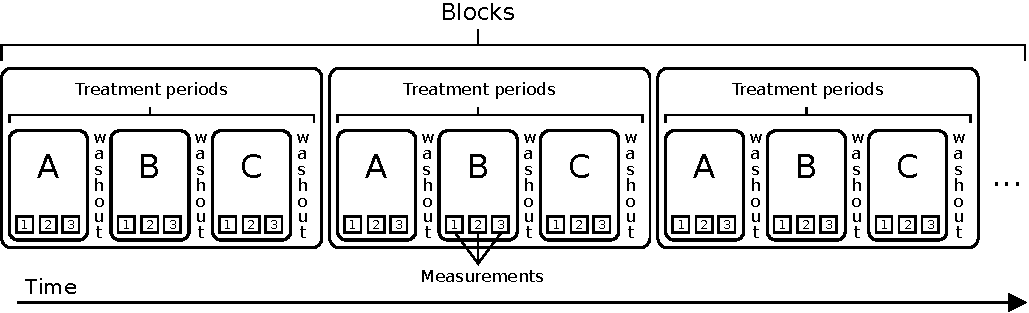
\includegraphics{n-of-1_schema.pdf}
\end{figure}

The stated aim of N-of-1 trials is quite different from RCTs: where the latter
tries to generalize results to the population and find which treatment is best in
general, the N-of-1 trial does not try to generalize beyond the patient in question.
This means that, whereas comorbidity and other factors that cause systematic
variation between the patients in treatment outcomes are a problem in RCTs,
these are not an issue in N-of-1 trials because there is no need to generalize
beyond the one patient. There is also often no actual need to know what is
causing a certain treatment to work better or worse, as long as it is not
because of measurement errors or time-related effects.

Use of N-of-1 trials is appropriate in situations where there are multiple
treatment options but no prior knowledge of which of these would be
best, when there is known to be considerable variability between patients in
treatment efficacy, or when there is reason to doubt that the results from
scientific literature generalize to the patient in question\ \cite{nofone}. This
would seem to make N-of-1 trials applicable to many situations, but there are
also multiple factors restricting their use.

Firstly, N-of-1 trials can only be used to study illnesses that are chronic,
progress slowly, and are at least somewhat stable. Additionally, the treatment options
available must have noticeable treatment responses within a short timeframe.
Running the trials takes time and fast-changing illness or slow
treatment onset would make it either impossible to distinguish true effects from
the natural progression of the disease or make the length of the trials
impractically long. N-of-1 trials are also unsuitable for testing
preventative treatments because the effects of these treatments are often
impossible to assess without comparisons to other patients who are not receiving
the treatment.\ \cite{nofone}

Secondly, running N-of-1 trials is costly because of added expenses of training
the medical staff in the method, running the trial with all its measurements and
analyzing the data. This means that it can be hard to find cases where using
this method is cost-effective and studies assessing the cost and benefits of these trials
have given mixed results\ \cite{costs}.

These limitations have kept the use of N-of-1 trials rare in clinical use, even
though they could potentially both increase the life quality of the patients and
lower the healthcare costs by finding the most suitable medications to patients that
might end up using them for years. This state of affairs might be
changing fast though. Ageing and environmental factors are changing the worlds'
disease burden so that a growing proportion of it is constituted by chronic
diseases\ \cite{diseaseburden}, of which common ones like non-acute cardiovascular
diseases and diabetes are excellent candidates for N-of-1 trials. Also, the costs
of administering N-of-1 trials are dropping with the advent of cheap and reliable
health sensors like smartwatches and connected blood pressure monitors. For
example, it is now possible to get real-time readings of
blood insulin levels with minimal effort from the patient\ \cite{cgm}. These
ongoing changes mean that the popularity of this method could potentially rise
significantly in the coming years.

\chapter{Statistical modelling of N-of-1 Trials}\label{modelling}

Even though the data created by the N-of-1 trials resembles traditional time
series data with autocorrelation between observations and repeated measurements
from the same study unit, additional complexities arise from the structure of
repeating treatment periods. Trying to take into account all
the peculiarities of the study design could end up with a model that is too complicated to
the small amount of data generated by a single study, so one must consider
carefully what factors need to be incorporated into the model.

Simplest model that we could employ is to just count the number of blocks where
a treatment is considered ``better'' than others. The precise definition of
``better'' doesn't matter here. This way we arrive to a simple binomial model
where the number of ``successes'' \(X\) is the number of blocks where a
treatment is considered the ``best'' follows binomial distribution and the
probability of each treatment option of having \(k\) successes is given by:

\begin{def}\label{}
    \begin{equation}
        P(X = k) = {n\choose k}p^k{(1-p)}^{(n-k)},
    \end{equation}
\end{def}where \(k\) = number of blocks, where the treatments is considered the
``best'', \(n\) = total number of blocks and \(p\) = the probability of being
considered the ``best''.

This type of model is rudimentary at best because it fails to consider the
magnitude of the differences between treatment effects and does not take into
account the actual number of measurements within each treatment period. To take
these factors into account, more complex models are in order.

\section{Basic Models}\label{conti}

Before going further we assume that the measurements we are dealing with are continuous
as this is probably the most common case. Let's first look at a model where
we assume that there are no time-trends and no autocorrelation between
measurements. Let \(y_{mbpt}\) represent the outcome measured while on treatment
\(m\) within treatment block \(b\) within treatment period \(p\) at time \(t\).
The treatment periods are indexed within each block and time is indexed within
each treatment period:

\begin{def}\label{}
    \begin{equation}\label{allerrors}
        y_{mbpt} = \mu_m + \gamma_b + \delta_{p(b)} + \epsilon_{t(p(b))},
    \end{equation}
\end{def}where \(\gamma_b \sim N(0,\sigma^2_{\gamma})\), \(\delta_{p(b)} \sim
N(0,\sigma^2_{\delta})\), and \(\epsilon_{t(p(b))} \sim
N(0,\sigma^2_{\epsilon})\)

This model assumes all treatment effects \(\mu_m\) to be constant. Within the
normally distributed terms, \(\gamma_b\) represents random block-effects,
\(\delta_{p(b)}\) random treatment period effects and \(\epsilon_{t(p(b))}\) random within
period errors. We could also choose one of the blocks as a reference and set
\(\gamma_1 = 0\) and assume that within each block the between period effects
follow the same pattern, i.e.\ he difference between treatment period one and
two is the same within each block. The random-effects between blocks and treatment
periods could represent for example the random variations in the motivation of the patient and possible
changes in treating personnel within each block and treatment period. The random
within period errors represents the measurement error of single measurements
within treatment periods. The relative size of these terms is important
for effective design of the trial because they determine if it is more
beneficial for the statistical power of the study to add more measurements,
treatment periods or blocks.

If the measurements within blocks and treatment periods do not correlate, the
model\ \ref{allerrors} can be greatly simplified by dropping \(\gamma_b\) and
\(\delta_{p(b)}\):

\begin{def}\label{}
    \begin{equation}\label{oneerror}
        y_{mbpt} = \mu_m + \epsilon_{t(p(b))},
    \end{equation}
\end{def}where \(\epsilon_{t(p(b))} \sim N(0,\sigma^2_{\epsilon})\).

This simple model could be considered a starting point in modelling a successful trial where
the treatments and measurements were administered consistently, there were no big changes to the staff interacting
with the patient and no modifications to any other procedures were made during
the trial.

\section{Incorporating time-trends into the model}\label{timetrends}

As the symptoms of the patient might not be completely stable (e.g.\ because
symptoms get worse with the progression of the disease) adding some kind of
time-trend to the model is usually advisable. We can modify the simple model\ \ref{oneerror} from previous Chapter to include a linear time-trend by adding an
intercept and slope of the time-trend. In this case the model can be expressed more
concisely just in terms of the measurement \(y_t\) taken at time \(t\), where
time is indexed from the start of the study:

\begin{def}\label{}
    \begin{equation}\label{simpletimetrend}
        y_t = \beta_0 + \beta_1 t + \mu_m + \epsilon_t,
    \end{equation}
\end{def}where \(\epsilon_t \sim N(0,\sigma^2)\).

Here \(\beta_0\) is the intercept, \(\beta_1\) the slope of the time trend,
\(\mu_m\) the effect of the treatment given during time \(t\) and \(\epsilon_t\)
is the residual error at time \(t\). More complex time-trends can be introduced
by modifying the slope, for example by adding the term \(\beta_2 t^2\) to
introduce a quadratic trend.

Another time-dependent effect to take into consideration is period effects.
There might be some part of the trial that falls within a period that we presume
to have its own effect. An example of this kind of effect is if we study asthma
medications and part of the trial falls within the pollen season. A simple way
to model this is to use a dummy variable that takes the value 1 within the
period and 0 outside it. Extending the model\ \ref{simpletimetrend} with a period of constant
effect \(\beta_2\) we end up with:

\begin{def}\label{}
    \begin{equation}\label{}
        y_t = \beta_0 + \beta_1 t + \beta_{2}Z_t + \mu_t + \epsilon_t,
    \end{equation}
\end{def}where \(\epsilon_t \sim N(0,\sigma^2)\) and dummy variable \(Z_t = 1\)
when \(t \in (t_{period\,start} \ldots t_{period\,end}) \) and \(0\) otherwise.

Lastly, to take into account that treatment effects themselves can vary with
time, for example because treatment works better during periods of greater
disease severity, we can add a time-by-treatment interaction effect into the
model. For example in the case where we expect that the illness gets steadily
(linearly) worse with time, but the treatments compensate this by being
similarly more effective, we can extend the simple linear
time-trend model\ \ref{simpletimetrend} by adding a second time related
treatment term \(\gamma_m t\) which describes the effect of treatment \(m \) given at
time \(t \) in regard to time:

\begin{def}\label{}
    \begin{equation}\label{}
        y_t = \beta_0 + \beta_1 t + \mu_m + \gamma_m t + \epsilon_t,
    \end{equation}
\end{def}

In general, systematic and complex time-related effects are difficult to
deal with in N-of-1 studies as the amount of data created is typically small
and complex parametrization can quickly lead to models that are impossible to estimate
effectively. Some of these problems can be avoided by good experiment design (for example not
conducting trials where we expect any period effects), but unfortunately this does not
help with illnesses that progress in complicated fashion and with the time-dependent
treatment effects related to this progress.

\section{The Problem of Autocorrelation}\label{autocor}

A common occurrence in time-series data is the autocorrelation between
measurements so that there is some similarity between observations defined by a
function of the time lag between them. Often a good first response to this problem
is to add a time-trend to the model as we did previously. This
often removes a substantial proportion of the autocorrelation that could be
caused for example by the natural progression of the disease\ \cite{stat}.
Unfortunately, in N-of-1 trials the carryover effects
from previous treatments and slow onset of treatment effects can lead to very
complex autocorrelation patterns that are hard to remove with just a simple time-trend.

Carryover effects refer to the lingering effects of the treatment even after it
has been stopped. This can make the treatment effects in the next treatment period
with a different treatment seem larger than they really are or smaller in the
unfortunate, and hopefully rare, case where the previous treatment was actually
harmful. Carryover effects also encompass the effects of interactions between
sequential treatments, which could even be dangerous depending on the nature of
the treatments. On the other hand treatment effects that manifest slowly can
often give the opposite effect of carryover effects by making the treatments
look less effective than they truly are during the first measurements of each
treatment period.\cite{stat}

To deal with these more devious sources of autocorrelation in our model we can
take two routes: moving average models and autoregressive models. In moving
average models the error is represented as depending on the previous error(s) by
expressing the measurement at time \(t\) as function of one or more previous
errors:

\begin{def}\label{}
    \begin{equation}\label{movingaverage}
        y_t = \mu_m + \epsilon_t + \rho\epsilon_{(t - 1)},
    \end{equation}
\end{def}where \(\mu_m\) is the effect of the treatment given at time t, \(\rho
\) is the correlation between consecutive errors and all errors \(\epsilon_t \sim
N(0,\sigma^2) \). Instead of making the measurement dependent on just the previous error, the model
can be adjusted to include a more complex lag by adding more error terms with
bigger lag and including more \(\rho \) terms to denote the correlations between
them (\(\rho_1\epsilon_{t-1} + \ldots + \rho_x\epsilon_{t-x}\)).

With autoregressive models, we express the autocorrelation in the
measurements themselves so that the measurement at time \(t\) is a function of
the measurement at \(t-1\):

\begin{def}\label{}
    \begin{equation}\label{}
        y_t = \rho y_{t-1} + \mu_m + \epsilon_t,
    \end{equation}
\end{def}where \(\mu_m\) is the effect of the treatment given at time \(t\),
\(\rho \) is the correlation between consecutive measurements and \(\epsilon_t
\sim N(0,\sigma^2)\) is the error term. Like with moving average model we could
also include more than just one lag by adding more lagged terms and correlation
terms. Although it can make more intuitive sense to make the whole observation
dependent on the previous observation as we do here, it is important to recognize
that then treatment effects \(\mu_m\) must be interpreted differently as they are
conditioned on previous measurements.

Moving average models and autoregressive models are often combined by using both
methods of taking the autocorrelation into account simultaneously (ARMA-models), but as
amount of data produced in N-of-1 studies if often so small, taking this approach might
not be advisable as it might make the model too complex.

Although we can try to solve the problems created by the carryover effect and the slow
manifestation of treatment effect with modelling, a better way could be to mitigate the
effects with the study design itself. By having a long
enough washout period between different treatments, we can minimize the
carryover effect. If there are no harmful interactions between the treatment the
next treatment can be started within the washout period so that we minimize the
problem of slow treatment effects. If there are interactions to be taken into
consideration, the first few measurements at the beginning of each treatment
period could also just be dropped. By doing this we are of course throwing away
data, but we must remember that if the measurements at the beginning of the
treatment period are mangled, these will also mangle our parameter estimates.
Trying to take these effects into account in our model will probably not
eliminate them completely and will increase the complexity of our
model.

\section{Non-continuous Measurements}\label{noncontinuous}

Up to this point, we have assumed that the measurement used are continuous, but
we could have measurements that are binary, counts of events or
categorical. With these kinds of measurements the models need to be reformatted so that
they don't presume normal distributions. Despite this, the models don't
have to differ much from the models presented above and the principals covered
before can still be applied.

To modify previously presented models to work when measurements are not
continuous, we need to formulate them as generalized linear models. We do
this by keeping the right-hand sides in the same form but expressing the
left-hand side in terms of a link function of the mean of the probability
distribution of the outcomes. So instead of expressing the model in terms of
individual observations \(y_t\), we express it as the expected value of these
measurements conditional on the data that we feed to the link
function \(E(Y|D)\). The link function allows us to model measurements with arbitrary
distributions, as now the link function can linearly depend on the parameters of
the model, rather than needing the measurements themselves to do so. We need to
do this to prevent the models from giving impossible predictions, i.e.\ negative
counts or probabilities.

Let's start with binary outcome measurements. In this case the
measurements \(y\) at time \(t\) follow the Bernoulli distribution \(y_t \sim
Bernoulli(p)\) where the the expected value of the distribution is the
probability \(p\) of observing the event in measurement \(y_t\). In this case
the suitable link function is the logit function
\(logit(p)=\log_e(\frac{p}{1-p})\). With this information we can now formulate a
model with simple a linear time trend:

\begin{def}\label{}
    \begin{equation}
        \log_e(\frac{p_t}{1-p_t})=\beta_0 + \beta_1 t + \mu_m,
    \end{equation}
\end{def}where \(p_t\) is the the probability of observing the event at time
\(t\) and \(\log_e(\frac{p_t}{1-p_t})\) are the log-odds of this event,
\(\beta_0\) is the intercept, \(\beta_1\) the slope of the time trend and
\(\mu_m\) the effect of the treatment given during time \(t\). By first
exponentiating and then using simple algebraic manipulation we can
express the model in terms of the probability \(p_t\):

\begin{def}\label{}
    \begin{equation}\label{}
        \frac{p_t}{1-p_t}=e^{\beta_0 + \beta_1 t + \mu_m}
    \end{equation}
\end{def}

\begin{def}\label{}
    \begin{equation}\label{}
        p_t=\frac{e^{\beta_0 + \beta_1 t + \mu_m}}{e^{\beta_0 + \beta_1 t + \mu_m}+1}=\frac{1}{1+e^{-(\beta_0 + \beta_1 t + \mu_m)}}
    \end{equation}
\end{def}

One thing to pay attention here is that there are no error terms in the model. This is because we are
not modelling individual observations, but the expected value of these values, which in
this case is the probability of observing the event under treatment used at time \(t\).
Even though there are random variations in the individual observations,
when we talk about their expected value, there is just a single value with no
random errors. Apart from this difference, we can see that we find the same model
from the denominator that we used when modelling a continuous measurement with a
linear time-trend in model\ \ref{simpletimetrend}, but without the
aforementioned error term. This means that to build the models described before,
we would just insert the right side of the equations into the denominator,
leaving out the measurements error term.

With numbers of events as measurements, instead of expressing the model in terms
of time, we can express it in terms of periods \(p\) that are of equal length
and indexed from the beginning of the experiment (this should correspond to the
treatment periods as they should be of equal length). The number of events during
period \(y_p\) follows a Poisson distribution \(y_p \sim Poisson(\lambda)\) and
the expected value of the distribution is the rate \(\lambda_p \) of the events
during period \(p\). For link function we use the natural log so that we have
\(\log_e(\lambda_p)\) on the left side of the equation. Once again using the
same simple model with linear time trend we end up with a model:

\begin{def}\label{oneerror}
    \begin{equation}
        \log_e(\lambda_p)=\beta_0 + \beta_1 r + \mu_{p},
    \end{equation}
\end{def}where \(\lambda_p\) is the the rate of events between measurements
during period \(p\), \(\beta_0\) is the intercept, \(\beta_1\) the slope of the
time trend and \(\mu_p\) the effect of the treatment given during period \(p\).
By simply exponentiating both sides we can express the model in terms of rate of
events:

\begin{def}\label{oneerror}
    \begin{equation}
        \lambda_p=e^{\beta_0 + \beta_1 t + \mu_p},
    \end{equation}
\end{def}where we now have the familiar linear model formula in the exponent on
the right side of the equation.

The case of categorical measurements is more complex as there are multiple
possible link functions depending on which way we want to model the
measurements, so we don't go through all of them here. The one that is probably
the most relevant is the case when categorical measurements are ordinal, i.e.
they have a natural ordering like in a Likert-scale. In this case the we can
use the cumulative logit as the link function. So if we assume that our ordinal
measurement has \(J\) categorical choices ordered from 1 to \(J\), we can model
the cumulative probability of getting a measurement \(y\) at time \(t\) that is at
``smaller or equal'' to \(y\) by putting this to the logit function and using the same
basic model as before:

\begin{def}\label{oneerror}
    \begin{equation}
        \log_e\bigg({\frac{P(y_t \leq j)}{1 - P(y_t \leq j)}}\bigg)=\beta_0 + \beta_1 t + \mu_p,
    \end{equation}
\end{def}where \(\beta_0\) is the intercept, \(\beta_1\) the slope of the time
trend and \(\mu_t\) the effect of the treatment given during time \(t\). By
exponentiating and algebraic manipulation we end up with similar model as with
binary outcomes where we once again find the familiar linear model formula in
the exponent:

\begin{def}\label{}
    \begin{equation}\label{ord_exponentiating}
        \frac{P(y_t \leq j)}{1 - P(y_i \leq j)}=e^{\beta_0 + \beta_1 t + \mu_t}
    \end{equation}
\end{def}

\begin{def}\label{}
    \begin{equation}\label{ord_algmanipulation}
        P(y_t \leq j)=\frac{e^{\beta_0 + \beta_1 t + \mu_t}}{e^{\beta_0 + \beta_1 t + \mu_t}+1}=\frac{1}{1+e^{-(\beta_0 + \beta_1 t + \mu_t)}}
    \end{equation}
\end{def}

The general pattern here is that, even in the case when the measurements are not
continuous, all the modelling principals we introduced earlier still apply. The way we
think about how different parameters affect our measurements does not have to change,
even though the models need to be expressed differently.

\chapter{Bayesian Estimation}\label{bayes}

Now that we have some models defined, we need to give estimates to the parameters in these models. There
are two broad ways to approach this task by using two different definitions of
probability. The first is frequentist inference, where we consider the ``true''
parameters of our model fixed, but unknown, and probability only applies to the
process of creating our data. The second way is Bayesian inference, where we
consider the data as fixed and instead of thinking about the parameters as
fixed parts of nature, we conceptualize them as probability distributions that
express our uncertainty about their true values.

Although both of these inference methods work for all the models covered before,
several factors favour the use of Bayesian inference in N-of-1
studies because of to their design and use context. But before talking about these factors,
we need to understand how Bayesian inference works.

\section{Principles of Bayesian Inference}\label{whybayes}

Bayesian inference is based on the Bayes' Theorem that states the probability of
an event conditional on another event:

\begin{def}\label{}
    \begin{equation}\label{bayesrule}
        P(A|B) = \frac{P(B|A)P(A)}{P(B)},
    \end{equation}
\end{def}where \(A\) and \(B\) are events and \(P(B)\) \(\neq \) 0. \(P(A|B)\) is the conditional probability of event \(A\) happening given that
event \(B\) and is called the posterior. \(P(A)\) is our initial
probability estimate for the event \(A\) called the prior. The quotient
\(\frac{P(B|A)}{P(B)}\) represent how much information event \(B\) gives about
event \(A\). If this number is greater than 1, then event \(B\)
makes event \(A\) more likely and if it less than 1 event \(B\) makes event \(A\) less likely.
If the quotient is 1, event \(B\) gives no information about the probability of
event \(A\). Breaking the quotient down further \(P(B|A)\), called the likelihood, is the reverse of the posterior and tells us how believable it is to
see the event \(B\) given that event \(A\) happened. Finally, \(P(B)\) in the denominator is called marginal likelihood and tells us the probability of
observing event \(B\) with or without event \(A\).

In our case, instead of events, we want to formulate the theorem with parameters
\(\Theta \) and the data \(D\), so that we get an estimate of the posterior
probability (or likelihood in case of continuous parameter values) of our
parameters having certain values:

\begin{def}\label{}
    \begin{equation}\label{bayeswithparams}
        P(\Theta|D) = \frac{P(D|\Theta)P(\Theta)}{P(D)},
    \end{equation}
\end{def}where \(P(D)\) \(\neq \) 0. We could make it more explicit what the marginal likelihood \(P(D)\) stands for
by writing it as \(\sum_\Theta P(D|\Theta)P(\Theta)\) in the case when the parameter
value takes discrete values and \(\int_\Theta P(D|\Theta)P(\Theta) d\Theta \),
if they are continuous. That is, the possibility of observing the data with all
different combinations of the possible values of the parameters, taking into
account our prior beliefs in the probability of these value combinations.

To tie this formula into the models we introduced previously we can demonstrate
how this applies to a simple model with only the treatment effects \(\mu_m \) of
the given treatment and a random error \(\epsilon \) at time \(t\):

\begin{def}\label{}
    \begin{equation}\label{}
        y_t = \mu_t + \epsilon_t,
    \end{equation}
\end{def}where \(\epsilon_{t} \sim N(0,\sigma^2)\). In this case when we want to estimate the parameters of the effects of the
treatments \(\mu_m\). For simplicity let's assume that only one treatment was
given so \(\mu_t\) is constant. Let's refer to this treatment effect simply as
\(\mu \). According to our model single observations follow a normal
distribution defined by constant \(\mu \) and the error term \(\epsilon_t \). As
our model assumes that the observations \(y_t\) are independent (no
autocorrelation included in the model) individual observations follow a normal
distribution \(y_t \sim N(\mu,\sigma^2) \) and the likelihood term in the bayesian formula is
a simple product of the probability density functions of a normal distribution
with mean \(\mu \) and variance \(\sigma^2 \):

\begin{def}\label{}
    \begin{equation}\label{}
        P(Y|\mu, \sigma)
        =
        \prod_{t=1}^{n}
        \frac{1}
        {{\sqrt {2\pi \sigma^2} }}
        \exp{ \left \{ \frac{-(y_t-\mu)^2} {2\sigma^2} \right \} },
    \end{equation}
\end{def}

To avoid the complexity of dealing with multiple unknown variables we assume
that \(\sigma \) is known. We will later come back to the case of multiple
unknown variables. Now we have to define only one prior distribution as there is
just one unknown parameter. We choose a normal distribution for the prior of
\(\mu \) that is defined by mean \(\lambda_0 \) and variance \(\delta_0^2 \),
which are values we define ourself based on our previous knowledge and beliefs:

\begin{def}\label{}
    \begin{equation}\label{}
        P(\mu)
        =
        \frac{1}
        {{\sqrt {2\pi \delta_0^2} }}
        \exp{ \left \{\frac{-(\mu-\lambda_0)^2} {2\delta_0^2} \right \} }
    \end{equation}
\end{def}

We could, of course, choose whatever distribution best matches our previous
knowledge and uncertainty about the parameter, but by using a normal distribution
for prior when the likelihood also follows a normal distribution, we get some
nice algebraic properties that we will soon see.

Now the only missing term from our bayesian equation is the marginal likelihood
\(P(Y) \). When we express the term more precisely as the probability of getting
the data we observed over possible values of our unknown parameter \(\int
P(Y|\mu,\sigma^2)P(\mu) d\mu \), we can see that as we integrate over all the possible
values of \(\mu \) and \(\sigma^2\) is known, this term is constant. This means that the marginal likelihood does
not affect the shape of the posterior distribution, So the shape of posterior
distribution is defined just by the likelihood and the prior \(P(\mu|Y)
\propto P(Y|\mu, \sigma^2)P(\mu) \). With some arithmetic manipulation we can
see that the posterior probability is actually a normal distribution with mean
\(\lambda_1 = \delta_1^2 \left( \lambda_0 \delta_0^{-2} + \sum_{t=1}^{n} y_t \sigma^{-2}
\right) \) and standard deviation \(\delta_1^2 =
\frac{1}{\delta_0^{-2}+n\delta^{-2}} \):

\begin{align}\label{normalposterior}
    P(\mu|Y) & \propto P(Y|\mu, \sigma)P(\mu)                                                                 \\
             & =
    \prod_{t=1}^{n}
    \frac{1}
    {{\sqrt {2\pi \sigma^2} }}
    \exp{ \left \{ \frac{-(y_t - \mu)^2} {2\sigma^2} \right \} }
    \frac{1}
    {{\sqrt {2\pi \delta_0^2} }}
    \exp{ \left \{ \frac{ -(\mu - \lambda_0)^2 } {2\delta_0^2} \right \} } \nonumber                          \\
             & =
    \frac{1}
    {
        (2\pi)^{\frac{n+1}{2}}
        \sqrt{ \delta_0^2 \sigma^{2n}}
    }
    \exp{
        \left \{
        \frac{- \mu^2 + 2 \mu \lambda_0 - \lambda_0^2}{2\delta_0^2}
        -
        \sum_{t=1}^{n}
        \frac{y_t^2 - 2 \mu y_t + \mu^2}{2\sigma^2}
        \right \}
    } \nonumber                                                                                               \\
             & \text{Dropping the constant terms} \nonumber                                                   \\
             & \propto
    \exp{
        \left \{
        \frac{
            -\mu^2 (\sigma^2 + t\delta_0^2)
            + 2 \mu (\lambda_0 \sigma^2 + \delta_0^2 y_1 + \cdots + \delta_0^2 y_n)
            - (\lambda_0^2 \sigma^2 + \delta_0^2 y_1^2 + \cdots + \delta_0^2 y_n^2)
        }
        {2\delta_0^2 \sigma^2}
        \right \}
    } \nonumber                                                                                               \\
             & \propto
    \exp{
        \left \{
        \frac{
            - \mu^2
            + 2 \mu \frac{\mu_0 \sigma^2 + \sum_{t=1}^{n} \delta_0^2 y_t}
            {\sigma^2 + n \delta_0^2}
            - \left(
            \frac{
                \lambda_0 \sigma^2 + \sum_{t=1}^{n} \delta_0^2 y_t
            }
            {\sigma^2 + n \delta_0^2}
            \right)^2
        }
        {
            2 \frac{\delta_0^2 \sigma^2}{\sigma^2 + n\delta_0^2}
        }
        \right \}
    }
    \times
    \exp{
        \left \{
        -\frac{
            \lambda_0 \sigma^2 + \sum_{t=1}^{n} \delta_0^2 y_t
        }
        {
            2 \delta_0^2 \sigma^2
        }
        \right \}
    } \nonumber                                                                                               \\
             & \propto
    \exp{
        \left \{
        -
        \frac{
            \left(
            \mu
            -
            \frac{
                \lambda_0 \sigma^2 + \sum_{t=1}^{n} \delta_0^2 y_t
            }
            {
                \sigma^2 + n \delta_0^2
            }
            \right)^2
        }
        {
            2 \frac{
                \delta_0^2 \sigma^2
            }
            {\sigma^2 + n \delta_0^2}
        }
        \right \}
    } \nonumber                                                                                               \\
             & =
    \exp{
        \left \{
        -
        \frac{
            \left(
            \mu
            -
            \frac{
                \lambda_0 \delta_0^{-2} + \sum_{t=1}^{n} y_t \sigma^2
            }
            {
                \delta_0^{-2} + n \sigma_0^{-2}
            }
            \right)^2
        }
        {
            2 \frac{1}
            {
                \sigma^{-2} + n \delta_0^{-2}
            }
        }
        \right \}
    } \nonumber                                                                                               \\
             & \text{Recognizing that we have the ''right'' part of normal distribution and adding} \nonumber \\
             & \text{the constant part back in} \nonumber                                                     \\
             & \propto
    \frac{1}
    {{\sqrt {2\pi \sigma^2} }}
    \exp{
        \left \{
        -
        \frac{
            \left( \mu - \lambda_1 \right)^2
        }
        {
            2 \delta_1
        }
        \right \}
    }, \text{ where } \nonumber                                                                               \\
             & \delta_1^2
    =
    \frac{1}{\delta_0^{-2}+n\delta^{-2}}
    \quad\text{and}\quad
    \lambda_1
    =
    \frac{
        \lambda_0 \delta_0^{-2} + \sum_{t=1}^{n} y_t \sigma^2
    }
    {
        \delta_0^{-2} + n \sigma_0^{-2}
    }
    =
    \delta_1^2
    \left(
    \lambda_0 \delta_0^{-2} + \sum_{t=1}^{n} y_t \sigma^{-2}
    \right) \nonumber
\end{align}

So we ended up with a posterior distribution that has the shape of a normal
distribution. The trick where we ignored the marginal likelihood can be used
anywhere, but the fact that we could arithmetically solve that the posterior
follows a well-defined distribution is not a general occurrence. Usually, we need
to go beyond arithmetic methods and solve the problem algorithmically.

\section{Challenges of Bayesian Inference}\label{bayesinferencechallenges}

Although the Bayes formula is conceptually simple, when utilizing
it we run into two big difficulties. First is the fact that
probability distributions of the likelihood (likelihood times prior) are often not
well-defined distributions with known properties. This makes the
integral in the marginal likelihood impossible to solve analytically as we did
above. With discrete distributions, we can circumvent the problem by just counting the
likelihood times prior for every value combination and then obtaining the posterior
probabilities by dividing each of these values with their combined sum. Unfortunately,
even here this becomes quickly impractical when the number of parameter combinations grows.
To be able to use the Bayes formula outside a narrow field of application we need to be able to solve the
problem of the marginal likelihood. The second problem is how we should define our priors.
If we have prior knowledge, we need to be able to
formulate our beliefs in a precise mathematic form. Even when we don't have prior knowledge we still
need to come up with a prior, but in this case, it has to be defined so that it has
minimal effects on the posterior distribution. When using informative priors we have to
ask ourselves if are these truly justified and with uninformative priors we have to deal
with fact that determining what prior is truly uninformative is often not straightforward.

\subsection{Dealing with the Marginal Likelihood}\label{marginallikehoodproblems}

As mentioned above, the marginal likelihood can often be impossible or
unfeasible to calculate analytically even in the case parameters with discrete
values where we don't need to solve a complex integral. A common solution to this,
that has been historically the only option, is to rely on so-called ``conjugate
priors``. These are priors that follow distribution which multiplied by
suitable likelihood function produce a posterior distribution that has the same
form as the prior distribution. A good example of this is our example above (\ref{normalposterior}) using a normal
distribution for the prior when the likelihood is also normally distributed. If
the likelihood function belongs to the exponential family of distributions, there
exists at least one corresponding conjugate prior distribution (often also in
the exponential family). For likelihood functions outside the exponential family,
there are some cases where a conjugate prior exists, but these are rare.

The conjugate function method makes the denominator analytically solvable, but it
is in practice very limiting. First, we need to restrict ourselves when
modelling to only use models that create a suitable likelihood function with an existing
conjugate prior. Second, it limits our options in defining our prior
beliefs as we have to be able to express them in the form of a conjugate distribution. To
be able to conduct Bayesian inference in cases where we can't conform to these demands we need
to turn to algorithmic solutions.

The basis for all algorithmic solutions to the problem is the fact that,
as the marginal likelihood is calculated over all possible parameter values, it is
not dependent on particular values of the parameter and is thus a constant value.
Therefore we can already know that the posterior will follow a distribution
with a shape that is defined by the likelihood times prior:

\begin{def}\label{bayespropto}
    \begin{equation}
        P(\Theta|D) \propto P(D|\Theta)P(\Theta)
    \end{equation}
\end{def}

Now if we could take a representative sample of values of this distribution we could
obtain an estimate of the posterior distribution by dividing the times we obtain a
certain value (or a value range) by the total number of samples. We can think of this
as estimating what is the probability of getting a 6 on
suspicious die by throwing it multiple times and counting which percentage of the
throws we get a 6. Doing this kind of sampling would be easy if the distribution would have
recognizable shape like a normal distribution, but in this case, we could already calculate an analytical
solution. The real problem is, how can we get a representative sample from an arbitrary
distribution. The general outline for the group of algorithms trying to solve this problem called
Monte Carlo Markov Chain (MCMC) goes as follows:

\begin{enumerate}
    \item Pick a set of values for our parameters as our starting position in
          the parameter space. The starting location has to be a plausible set
          of values. As we know that
          \(P(D|\Theta)P(\Theta)\) has the same shape as our posterior, if
          the value of this function is zero when we put our set of
          parameter values in it, these values are impossible and should not be
          uses as a starting point.
    \item Pick a second set of values for our parameters with some a random method.
    \item Calculate the probability of moving from our current position in the
          parameter space to the second set of parameter values with the
          following formula:

          \begin{def}\label{randomwalk}
              \begin{equation*}
                  p_{move\ to\ new\ location} = \min \bigg(\frac{P(D|\Theta = proposed\ set)P(\Theta = proposed\ set)}{P(D|\Theta = current\ set)P(\Theta = current\ set)}, 1 \bigg)
              \end{equation*}
          \end{def}

          In other words, if the likelihood times priors calculated with the proposed parameter
          value set is higher than the value for the current set, we always move
          to the new proposed location and if the value
          is lower we move there with a probability defined by the ratio of the
          two values.
    \item Generate a random number between 0 and 1 and move to the proposed
          location in the parameter space if the number is lower than the
          probability that we calculated in the previous step. Otherwise, we stay
          in the same place.
    \item Mark the parameter values of our current location in the parameter space.
    \item Repeat from step 2.

\end{enumerate}

After repeating this process multiple times we will end up with a list of values,
that are a sample of the distribution defined by the prior time
likelihood. With enough samples these values give us a good estimate of the entire
posterior distribution.

Why does this work? The crucial part in the algorithm is step 3. Consider a case
where we have just one parameter that can take two different values. Now the probability
of moving from one value to the other matches the relative values of the
target distribution and that means if value A is twice as probable as value B (if we don't know the
actual probability yet), the chance of moving from A to B is 50 \% and a chance of moving
from B to A is 100 \%. When we run the process of jumping from one to another, eventually each of our two values
will be visited proportionally to its value so we would expect the value to be A in 66
\% of cases and B in 33 \% of cases. We can demonstrate that this really happens with a short Python
example:

\begin{pyblock}[][fontsize=\footnotesize]
import numpy as np

np.random.seed(123)
steps = 10000
values = ["A", "B"]
sample = []
position = "A"

for i in range(steps):
    if position == "A":
        prob = np.random.random()
        if prob > 0.5:
            sample.append("B")
            position = "B"
        else:
            sample.append("A")
    else:
        sample.append("A")
        position = "A"

prob_a = sample.count("A") * 100 / steps
prob_b = sample.count("B") * 100 / steps

print(f"probability A: {prob_a} \%, probability B: {prob_b} \%")
\end{pyblock}
\stdoutpythontex
\bigskip

This logic extends to the case where we have
continuous values and also the case with multiple parameters. The formal proof
of this process is somewhat involved so we will skip it here and interested readers are
advised to check Chapter 7 in John Kruschke's Doing Bayesian Data Analysis\ \cite{kruschke}.

The second critical part of the algorithm is step 2 where we randomly create a new
position in the distribution where we will consider to move. In principal any kind of
random value picker works here as long as the it still possible to cover the whole
posterior distribution with sequential steps. The problem is
that with a bad algorithm this could take a long time. What we would want to have is a
way to create proposed steps that are rejected as rarely as possible and where the
jump from one value to another is as big as possible. These goals are in
conflict, so the algorithm has to find some optimal balance between them.
Having less rejection and taking bigger steps both lead to lower the autocorrelation
between consecutive samples which in turn leads to more efficient estimates by increasing the
effective sample size. There are different ways to calculate this metric, but roughly
these all measure the number of steps divided by the autocorrelation between the steps.
Why this is important can be intuited by thinking of comparison between a truly
random sample from a distribution and a sample where sampled values are only accepted if they are within a certain distance of the
previous sampled value or we take the same value again. It is clear that values created
with the former method are much better for
estimating the parameters of the distribution as the value from the later method might
end up bunched in only a small part of the distribution if the amount of samples is not
high enough. But the larger the value range for the next value is (i.e. proposed step
size), the closer the limited sampling method will match the truly random samples.

The simpler algorithms used for solving the problem of step proposal are still easily explainable, but
this part of the algorithm has seen some major improvement in recent years and the
current widely used solutions are technically much too complex to cover here. The
current ``industry standard'' is an algorithm called no-u-turn-Sampler (NUTS)\ \cite{nuts}
that could be heuristically described as choosing the values by rolling a frictionless
ball on terrain defined by the inverse of our distribution while at the same time
avoiding inefficient u-turns\ \cite{kruschke}. The algorithm can dynamically adjust the
size of the steps it takes to maintain a targeted step acceptance rate and, as estimates of
the posterior gets better, the steps are made bigger as more probable values will be
picked. Understanding how this works in practice is not an exercise for the faint of heart.

\begin{figure}[H]
    \centering
    \caption{First 100 Steps When Estimating Two Parameters With the NUTS Sampler}\label{traceexample}
    \includegraphics{trace_draw_example.pdf}
\end{figure}

To make it concrete how modern modern value proposal algorithms work, we
have visualized the first 100 steps taken by the aforementioned NUTS sampler
when estimating two parameters (figure\ \ref{traceexample}). The starting value is
marked with a black X and the markers turn from red to yellow as the chain progresses.
We can see that there seems to be a clear correlation between the parameters and our
sample is already reflecting that. If we look at the sizes the steps that the algorithm
takes, we can see that these are larger in the less probable parts of the distribution.
This means that the proposed step size also depends on where on distribution the current position
is located. With this intelligent sampling method, the chain traverses more
quickly in distribution and makes the sampling much more efficient than with older more
simple methods.

\subsection{How to Define the Priors?}\label{bayesproblems}

For the Bayesian formula to work we have to define a prior and this can be
trickier than it seems at first glance. Ideally the prior would codify our prior
beliefs and knowledge, but trying to rigorously codify everything we
know is often impractical, because of how complex this gets and we should aim lower as we are
anyway working with a model that should be a simplified representation of reality\ \cite{gelman}. Even if
we aim for a more limited goal, codifying our existing knowledge and beliefs
to mathematic formulas can be a tricky business. It gets even more
tricky when we consider that we are often doing the study not just to convince ourselves
but also other people and we should try to capture the beliefs of our target audience.
Unless this target audience is easily available for questions and is highly mathematically minded,
this leads to multiple layers of uncertainty as we try to guess what others
believe and then codify these beliefs with mathematical precision.

To avoid this hurdle the other option is to try to define some non-informative
priors that ``let the data speak for itself'', but this approach also has
problems. Firstly, defining priors that have no effects on the posterior can be mathematically
very difficult when we move beyond simple models and if we would need
to invest a lot of time finding these priors, we should instead probably spend this time
to define proper informed priors. Second, non-informative priors do not always
seem so non-informative when we actually know something about the issue.
Consider a case where are trying to predict if a patient has a rare disease
and we assign a uniform prior from 0 to 1 as this seems maximally non-informative. This
prior will have the effect of moving the posteriors towards the
possibility of the patient having the disease and the results could be nonsensical. So if we definitely know
something about the phenomenon, a non-informative prior can work against these
beliefs and give weird results.\ \cite{gelman}

Considered more broadly, chasing after truly non-informative prior is also
somewhat of a fool's errand if the data really has ``something to say''.
If the data is informative, then lots of different priors that are somewhat weak
should lead to almost identical posterior distributions. On the other hand, if the data is weak and we
have a weak prior, why are we even doing the analysis if we know that it will
give us almost no information?\ \cite{gelman}

As a compromise between having strong priors based on previous beliefs and knowledge and
letting the data stand on its own, Gelman et al.
suggest using weakly informative priors\ \cite{gelman}. These can be defined in two different
ways. Firstly, we can start with non-informative prior (when it is easily
available) and then add minimum information constraining the posterior results
to reality (e.g.\ object cannot move faster than light or the height of an adult human
must be between 50 and 300 cm). The other way is to start with strong informative
priors and then broaden these to take into account the uncertainty of
how applicable our priors knowledge is to the question at hand. A model defined in this
way should always be considered as provisional and we should pay close attention to the
reasonability of the posterior estimates. If the estimates don't make sense, this means
that we need to add stronger prior information, which we must hold as we would not be
able to evaluate the prior like this. This process should be repeated until we end up with
a model with just enough prior information to produce reasonable estimates.

Because of how complex defining priors can get, this problem can act as a limiter on
how complex Bayesian models we can build. The more complex model, the more priors we
have to define and the more prior information and beliefs we could codify and
the more difficult this problem gets. As there is no obvious universally applicable
solution to how we should create our priors, we have to make decisions case by case,
keeping in mind the existence of strong prior information, the needs of our model and
what makes sense to us and our target audience.

\section{Why Bayesian Inference Fits N-of-1 Studies}\label{whybayes}

As was mentioned before, both frequentist and Bayesian inference can be used to
estimate the parameter values of the types of models we described
in Chapter\ \ref{modelling}. The choice between these two methods is not just a
technical one as both come with different conceptions about the nature of probability
and these have serious implications on how we should interpret the results and run the studies.
Unfortunately for frequentist inference, its assumptions fit the reality of running
N-of-1 trials poorly, and its results can be hard to communicate to a lay
audience (in our case doctors and patients). Because of these issues, Bayesian inference
can usually be recommended over frequentist inference when analyzing and
communicating the results of N-of-1 studies, even though it comes it with its'
own complexities that we previously went over.

\subsection{Flexibility of Experimental Design}\label{whybayes}

The central tenet of frequentist inference is the assumption that same the
experiment could in theory be repeated with statistically independent results. Probability
is defined in relation to these hypothetical repetitions as a proportion of them
that would have some event of interest (e.g.\ over 5 tails with 10 coin tosses).
To repeat the same experiment its design needs to be defined precisely and this
definition needs to be made before the study has begun because the changes made
to the design during the experiment might be influenced by its results.

Let's consider an experiment where we are trying to find out if a coin
is fair with frequentist methods. For this purpose, we decide to flip the coin 20 times
and count the number of heads. After this, we model how ``typical'' the result we got
would be for a fair coin. We do this by calculating the distribution of heads from
multiple 20 coin toss trials
assuming that the coin is fair. Then we can compare our actual result against this
distribution. If our result seems like a typical sample from this distribution, we
can say that the null hypothesis stands and the coin is fair. Thus far we have no
issues. The problem comes if we did not decide to throw the coin 20 times
beforehand, but first threw it 10 times, looked at the results, though that we
should get some more data, and then threw the rest 10. Now what
kind of distribution should we compare our results against? The length of the trials
seems to now hinge in some undefined way from the results of the first 10 coin tosses
that made us decide to keep tossing the coin some more. For frequentist inference to
work our experiment design has to be clearly defined beforehand and we cannot make
unexpected changes to the experiment based on the data we get or any other factors.

This demand for predefined experiment designs is problematic in N-of-1 studies
used in a clinical setting. There might be cases when some treatment clearly seems
better in the middle of an experiment and the patient (or the clinician)
wants to stop the experiment. As the subjects are real people, it would be
unethical to force them to continue the study just for the sake of statistical
rigour. There might also be a situation where a couple of treatments seem
promising, but the rest seem completely useless, and we would want to change the
design of the experiment on the fly to focus just on the promising treatments.
These changes to the predefined experimental design will brake frequentist
assumptions and make getting non-biased inferences with this method impossible.

The option to stop the study or change the experimental design can be
incorporated to frequentist inference if we predefine the rules for when to
stop the experiment and under what circumstances the design should be altered
and how. Then we need to take these rules into account when performing the estimation
calculations which adds complexity but is still possible. The problem is that it is
questionable if we can stick to these rules because of
the human element: we would need to convince the patient that she should
stop the experiment only in these predefined circumstances. This seems quite
unrealistic, as if there are any unforeseen problems with the treatments, it is
more than likely that the patient will want to stop regardless of any rules she
signed up to follow beforehand.

With Bayesian inference doing on the fly modifications of the study design do not
cause such problems as with frequentist inference, as there is no assumption
about repeating the experiment. Instead of hypothesizing about future
experiment, we just take into account our prior information and the data created by
the current experiment. The changes to the experimental design modify what data
we get out of it, but don't break any assumptions of Bayesian inference. This
adaptability is a big benefit when applying N-of-1 designs in a clinical setting, as
the unpredictable nature of the patients and treatment effects and all the other
practical considerations that force changes to our experiment design don't
break the assumptions of the inference method.

\subsection{Richness and Communicability of the Estimates}\label{whybayes}

In N-of-1 studies much consideration has to be given to the communication of the
results both to the patient and the clinician administering the experiment. We
would like to portray not just the estimates of the effects of the treatments,
but also the uncertainty associated with these estimates. In frequentist
inference, we communicate these with maximum likelihood estimates, confidence
intervals and p-values. Maximum likelihood estimates are point estimates of the most
likely value and easily understandable, but don't communicate any uncertainty by themselves. With confidence
intervals, we can communicate uncertainty but don't actually mark the most likely
values of the estimate. A 95 \% confidence interval is often interpreted wrongly
as including the true value of the parameter with 95 \% change, but the real
meaning is that if we repeated the experiment indefinitely 95 \% of the
95 \% confidence intervals would include the true parameter value. This is
because, in frequentist interpretation of probability, true parameter values
are not random but fixed, so a single confidence interval either does or does
not include the true value. This confusing definition makes confidence intervals
a poor choice of presenting the uncertainty of the estimates to a lay audience
as they might create lots of misinterpretations and even when interpreted correctly
are hard to grasp. The second frequentist tool for communicating uncertainty
are p-values of hypothesis tests. We might define a null hypothesis that the
parameters of the effects of different treatments are equal and calculate the
likelihood to obtain the data or a more extreme version of it if this is indeed the
case. This would give us a more easily communicable way to portray the uncertainty
associated with results. If the p-value is low we could say with confidence that there are
real differences between the effectiveness of the treatments. The problem is that this actually gives us very little useful
information, as we would also like to how big the differences in the treatments' effectiveness
could realistically be.

A Bayesian approach to inference gives us richer and more easily communicable
information about the estimates because it gives the estimates in the form of the
posterior distribution. With this is we can easily point out the plausible values
with the tops of this distribution and the uncertainty with how flat the
distribution is. The usual misinterpretation of the confidence intervals as
containing the true value of the parameter with a certain probability is actually
the right interpretation for Bayesian credible intervals, that contain certain
percentage of the probability mass of the posterior distribution and so have a
defined chance of containing the true value of the parameter. Bayesian method itself
also seems to fit really well with the ways that clinicians conceptualize
their practice of arriving at diagnosis for a patient as updating their beliefs
(i.e.\ priors) with the new information gained from new observation such as test
results\ \cite{clinbayes}.

\chapter{Combining Information From Several N-of-1 Trials With Hierarchical Models}\label{hierarchicalbayes}

Let's say we have our N-of-1 trial set up nicely and we have a good model for analyzing the
results. After running the first trials, we continue to perform the same kind of setup
with multiple patients, as the treatments we are considering seem to have lots of
individual variation in their effectiveness. Running these experiments separately is
fine, but one might wonder if these separate trials could somehow be combined. Of
course, we could pool the data and run a group-based
analysis about what treatments seems to be the best in general, but there is a better
way that keeps true to the goal of N-of-1 experiments of finding the best treatment for
each individual patient by using Bayesian hierarchical models. In these models the
patient-level parameters are connected by imaging them as coming from a higher level
distribution. In the case of N-of-1 studies, we can think of a population-level distribution
where the patient-level parameters are drawn from. This makes lots of sense as it is
clear that, for example in the case of drug effectiveness, different people have different
effects, but these effects should follow some distribution with most people clustering around a
shared mode. In a sense having a common prior for
all patient-level parameters can already be thought as defining this population-level
distribution, but the difference is that, whereas the prior
is set in stone, the population-level
distribution in a hierarchical model works just like the patient-level
parameters with uncertainty included and thus it is possible that our beliefs (posterior
estimates) about this distribution will be changed by the data. Just like in the case of
informative shared prior,
the estimates of this population-level distribution can draw the
patient-level estimates closer together by making values from the distribution centre less
likely, but now the distribution is itself
estimated from the data and the strength of this effect depends on how similar the
observations from different and patients really are.

\section{How to Make a Model Hierarchical?}

The practicalities of hierarchical models are easier to explain if we conceptualize
Bayesian
models as trees. In the top of the tree we have prior values that define the shape of
prior distribution next level down, from these distributions come the parameters that
define the data creation process at the bottom of the tree. Let's take an example
where we have \(p\) patients with \(n\) measurements and, to make things simple, just
one treatment option. We can model this by a simple two-parameter model:

\begin{def}\label{}
    \begin{equation}\label{simplehierachical}
        y_{tj} = \theta_j + \epsilon_{tj}, i\in(1 \dots n), j\in(1 \dots p)
    \end{equation}
\end{def}where \(\theta_j\) represents the effect of the treatment for patient $j$ and
\(\epsilon_{tj} \sim N(0,\tau_j^2)\) is the error term for patient $j$ at observation
taken on time $t$. Now let's look at this model as a tree graph:

\bigskip
\begin{equation}\label{unpooledmodelexampletree}
\begin{tikzpicture}

    \matrix[matrix of math nodes, column sep=0pt, row sep=30pt] (mat)
    {
        \ & \mu, \sigma, \gamma & \ \\
        \theta_1, \tau_1 & \ldots & \theta_p, \tau_p \\
        y_{1,1}, \ldots, y_{n, 1} & \ldots & y_{1, p}, \ldots, y_{n, p} \\
    };

    \draw[->,>=latex] (mat-1-2) -- (mat-2-1);
    \draw[->,>=latex] (mat-1-2) -- (mat-2-3);

    \draw[->,>=latex] (mat-2-1) -- (mat-3-1);
    \draw[->,>=latex] (mat-2-3) -- (mat-3-3);

    \node[anchor=east] at ([xshift = -35pt]mat-1-1)
    {};

    \node[anchor=east] at ([xshift = -35pt]mat-2-1)
    {$\theta_j \sim \text{N}(\mu, \sigma^2), \tau_j \sim \text{HalfCauchy}(0, \gamma)$};

    \node[anchor=east] at ([xshift = -35pt]mat-3-1)
    {$y_{tj} \sim \text{N}(\theta_j, \tau_j^2)$};

\end{tikzpicture}
\end{equation}
\bigskip

For the prior distributions, we chose a normal distribution for the treatment effect and half-Cauchy
distribution centred on 0 for the variance where the scale parameter \(\gamma \) is the median of
the variance we expect. The
normal distribution for the treatment effect is a natural choice as probably the
treatment effect is dependent on multiple factors which many could be independent. If
this is the case, then the central limit theorem says that the treatment effect will follow a
normal distribution. The variance parameters are more difficult and there are multiple
reasonable distributions to choose, but half-Cauchy distribution is
recommended when we have some prior information is available\ \cite{variancepriors}.

Even though in this model each patient shares the same prior parameters, the estimates of the patient-level parameters
are only affected by the data of the patient in question as the shared prior parameter values are set
beforehand and are not affected by the data. You can think this as a model in which we have
perfect knowledge of the population-level distribution where the patient-level
parameters are drawn from and we describe this information with our priors.
To introduce flexibility about the population-level we need to
change the model so that the current prior-level is also being estimated based on
the data. We can accomplish this by changing the previous prior level from a set of values to distributions
that are themselves defined by a new higher level prior values:

\bigskip
\begin{equation}\label{hierarhicalmodelexampletree}
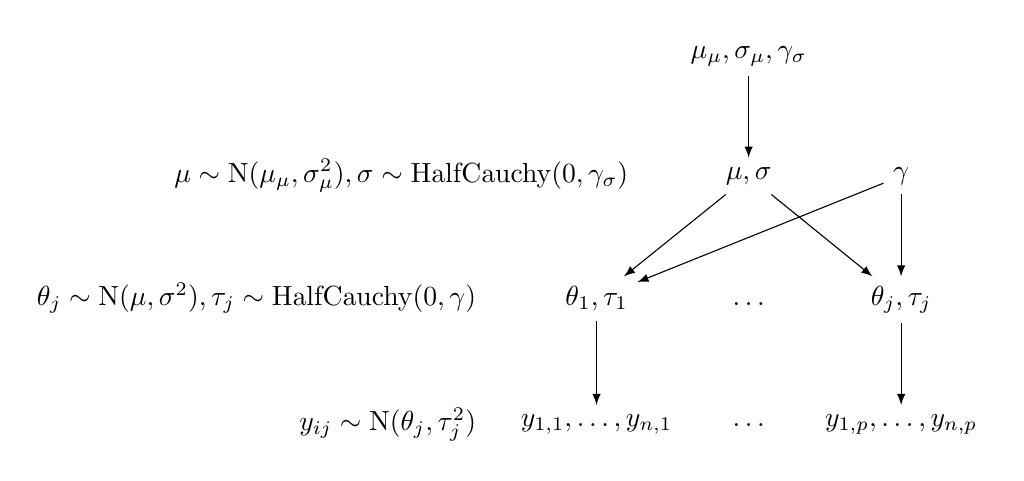
\begin{tikzpicture}

    \matrix[matrix of math nodes, column sep=0pt, row sep=30pt] (mat)
    {
        \ & \mu_{\mu}, \sigma_{\mu}, \gamma_{\sigma} & \ \\
        \ & \mu, \sigma & \gamma \\
        \theta_1, \tau_1 & \ldots & \theta_j, \tau_j \\
        y_{1,1}, \ldots, y_{n, 1} & \ldots & y_{1, p}, \ldots, y_{n, p} \\
    };

    \draw[->,>=latex] (mat-1-2) -- (mat-2-2);
    \draw[->,>=latex] (mat-2-2) -- (mat-3-1);
    \draw[->,>=latex] (mat-2-2) -- (mat-3-3);
    \draw[->,>=latex] (mat-2-3) -- (mat-3-1);
    \draw[->,>=latex] (mat-2-3) -- (mat-3-3);
    \draw[->,>=latex] (mat-3-1) -- (mat-4-1);
    \draw[->,>=latex] (mat-3-3) -- (mat-4-3);

    \node[anchor=east] at ([xshift = -40pt]mat-2-2)
    {$\mu \sim \text{N}(\mu_{\mu}, \sigma_{\mu}^2), \sigma \sim
    \text{HalfCauchy}(0, \gamma_{\sigma})$};
   
    \node[anchor=east] at ([xshift = -40pt]mat-3-1)
    {$\theta_j \sim \text{N}(\mu, \sigma^2), \tau_j \sim \text{HalfCauchy}(0, \gamma)$};

    \node[anchor=east] at ([xshift = -40pt]mat-4-1)
    {$y_{ij} \sim \text{N}(\theta_j, \tau_j^2)$};

\end{tikzpicture}
\end{equation}
\bigskip

Now instead of drawing the treatment-related patient-level parameters straight from distributions defined
by the priors, these are drawn from the population-level distributions. As the
parameters of the population-level distributions are now longer set in stone, they are
estimated based on the data and this way data from one patient can affect the estimates
of another patient by changing our beliefs of this shared layer.

The parameters of the population-level distributions now have prior values expressing our
uncertain knowledge and uncertainty about these distributions. The exception to this pattern is the error
term \(\tau \). We could make this parameter hierarchical, but this is not commonly done in hierarchical models. There are
two reasons for this. Firstly, this term is already ``extra'' in the model describing
the variance left after the more interesting parameters have been fitted. Compared to the actual
treatment effect this makes it less interesting and adding hierarchical layers for this
parameter can be thought of as unnecessary complexity. The second reason is that with a
reasonable amount of observations, the error term can be estimated very accurately from
the data. This means that adding the hierarchy should not have much effect on this estimate as the
patient-level estimates are likely too strong to be swayed by the population-level
estimates.

\section{Benefits of Hierarchical Models}

The kinds of multilayered dependencies introduced by hierarchical models are useful in many ways.
Firstly, the dependencies can be meaningful for the application, i.e.\ we can
model the treatment effect for a single patient as an instance from a
broader population distribution of this effectiveness. The population-level is not just
a mathematical curiosity here, but it has a meaningful interpretation and the estimates we
get for the population-level parameters are interesting by themselves. Secondly, because
of the dependencies across parameters, all the data can now jointly inform all the
parameter estimates. As there is now more data used for the lower-level estimates through
pooling, there is usually some reduction in the variance of these estimates
and especially between them. This reduction of variance is
generally referred by the term ``shrinkage''. In general,
shrinkage in hierarchical models causes lower-level parameters to shift toward the modes
of the higher-level distribution. This does not mean that
estimates are always just pulled closer together, because if the higher-level
distribution has multiple modes, then the low-level parameter values cluster
more tightly around these modes, which might push some
low-level parameter estimates apart instead of pulling them together. The greatest thing
is, that as we don't explicitly set the parameter values of the higher-level
distributions, the amount of shrinkage is informed by the data so that
similar observed data points from lower-level distributions lead to ``tighter''
estimates for the higher-level distributions and in this, in turn, leads to
greater shrinkage. This means that using a hierarchical model in the case where the
patients actually are very different, does not force the estimates together as
widely spread measurement values leads to the estimates of the population-level-distributions to
have a large variance and thus to have little impact on the patient-level estimates. So
instead of forcing similarity, the model ``makes the decisions'' if this is appropriate
based on the data (and our priors, as strong priors might force or prevent this effect).

\section{Applying the Bayes Formula to Hierarchical Models}

With all the parameters introduced by the new parameter levels in hierarchical models,
the question now becomes, how we apply
the Bayesian formula in these cases? Luckily this happens to be very simple as we just
have to remember two rules of probability: the chain rule\ \ref{chainrule}, that
tells us that the probability of \(A\) and \(B\) is the probability of \(B\) on condition \(A\)
times the probability of \(A\), and the rule of independence\ \ref{ruleofindependence}
that states that the
probability of \(A\) on condition \(B\) is just the probability of \(A\) if \(A\) and
\(B\) are independent.

\begin{equation}\label{chainrule}
    P(A \cap B) = P(B|A)P(A)
\end{equation}

\begin{equation}\label{ruleofindependence}
    P(A|B) = P(A), \text{ if } P(A \cap B) = P(A)P(B)
\end{equation}
\smallskip

Now let's see what happens when we include are our previously defined hierarchical
model\ \ref{hierarhicalmodelexampletree} in the Bayes formula\
\ref{bayeswithparams} and apply these rules:

\begin{equation*}\label{}
    \begin{aligned}\label{conjugatebayesrule}
        &P(\theta_1,\tau_1,\theta_2,\tau_2,\mu,\sigma | Y) \\
        &= \frac{P(Y | \theta_1,\tau_1,\theta_2,\tau_2,\mu,\sigma)P(\theta_1,\tau_1,\theta_2,\tau_2,\mu,\sigma)}{P(Y)} \\
        &\text{(dropping the constant term)} \\
        &\propto P(Y | \theta_1,\tau_1,\theta_2,\tau_2,\mu,\sigma)P(\theta_1,\tau_1,\theta_2,\tau_2,\mu,\sigma) \\
        &\text{(using rule of independence as data Y depends only on parameters $\theta$ and $\tau$)} \\
        &= P(Y | \theta_1,\tau_1,\theta_2,\tau_2)P(\theta_1,\tau_1,\theta_2,\tau_2,\mu,\sigma) \\
        &\text{(using rule of independence to separate the two patients)} \\
        &= P(Y_1 | \theta_1,\tau_1)P(Y_2 | \theta_2,\tau_2)P(\theta_1,\tau_1,\theta_2,\tau_2,\mu,\sigma) \\
        &\text{(using the chain rule to separate the patient and population parameters)} \\
        &= P(Y_1|\theta_1,\tau_1)(Y_2|\theta_2, \tau_2)P(\theta_1,\tau_1|\mu,\sigma)P(\theta_2,\tau_2|\mu,\sigma)P(\mu, \sigma)^2 \\
        &\text{(population parameters are independent of each other)} \nonumber \\
        &= P(Y_1|\theta_1,\tau_1)(Y_2|\theta_2, \tau_2)P(\theta_1,\tau_1|\mu,\sigma)P(\theta_2,\tau_2|\mu,\sigma)P(\mu)^2P(\sigma)^2 \\
        &\text{($\theta$ and $\tau$ are independent on each other and $\tau$ is not dependent on} \\
        & \text{population-level parameters)} \\
        &= P(Y_1|\theta_1,\tau_1)(Y_2|\theta_2, \tau_2)P(\theta_1|\mu,\sigma)P(\tau_1)P(\theta_2|\mu,\sigma)P(\tau_2)P(\mu)^2P(\sigma)^2 \nonumber
    \end{aligned}
\end{equation*}

We have now successfully expressed our hierarchical model in the Bayes formula.
We can see that the measurements of each patient \(Y_1 \) and \(Y_2 \) depend directly
only on the patient-level parameters \(\theta_1, \theta_2, \tau_1, \tau_2\), so that if these values are set, then the
measurements are independent of all other parameters. Similarly, \(\theta_1, \theta_2 \) depend conditionally only
on the population-level parameters \(\mu, \sigma \), while \(\tau \) is independent of
them. We could continue by writing the
formula out by adding in the prior terms and replacing the abstract probability
markings with the actual probability density functions given by our chosen
distributions, but this gets messy and, in this case, no nice analytical solution can be
found anyway, so we will leave it at this. Notably we could add even
more layers to the model and just apply the same rules we used here to write the formula
out. Bayes formula makes no limitations on how complex and deep our hierarchical model
can be.

\chapter{Example of a Hierarchical Bayesian Analysis Using Simulated Data}

To put everything we learned into practice let's go over an example Bayesian
analysis of multiple N-of-1 trials, where we first analyze one trial separately and then
combine multiple trials by using a hierarchical model. For the analysis, we use Python and PyMC3 library\ \cite{pymc3} built
for probabilistic programming. We will not go over each part of the code used, but focus only
on the critical parts where we see how the principals we went over in the
previous Chapters look like when implemented in practice. For those who want to see the
full code, it is available from a GitHub repository\ \cite{github} with instructions on how
to run it.

As we now jump theory to practice we will need to revisit the concepts that we went over
while talking about the problems of dealing with marginal likelihood\
\ref{marginallikehoodproblems} and introduce some new concepts related to how
PyMC3 deals with this problem and what we need to pay attention to
make sure that the algorithmically derived results we get are reliable. We also have to
consider how we can make sure that our model is a ``good enough'' description of reality.
Almost any kind of model can be fitted to the data and most of these can be even
estimated correctly, but only a few models describe the data generating process in an
accurate enough manner. To answer this question we need to introduce totally new concepts
relating posterior predictive checks, where we create new data based on the estimated
posteriors and see if this data looks like our original dataset.

\section{Defining the Experiment}

Let's first describe our experiment design, as this is critical for understanding
everything that comes later. Imagine that we have 6 patients that all suffer from the
same medical condition to which there are two treatment options available (A and
B). We know from the
literature that there is lots of patient-level variation in which treatment works better
so we decide to test this with N-of-1 trials. We know that both of the treatments act
very fast and that there are no known problems with interaction effects between them.
The state of the condition can also be easily measured at home so no visits to
a hospital is needed to take the measurements. Higher measurements mean worse condition
so we would like to find the treatment that gives the lowest measurements for each
patient. The condition is usually steadily
worsening with or without the treatment and the treatment is more for slowing down the
disease and not curing it. Based on this information we come up with the following experiment design:

\begin{itemize}
    \item The trial will run for 4 weeks with 2 weeks spent on each treatment
    \item Treatment periods will be one week long
    \item The week-long treatment periods will be organized into two blocks, each of
    containing one treatment period on treatment A and another on treatment B
    \item For each patient, the sequence of the treatments in the first block will be randomized and then
    the second block will have the treatments in reverse order creating a balanced
    design of either ABBA or BAAB
    \item Measurements will be taken by the patient at the end of each day so we will end up with
    28 measurements per patient with 14 for each of the treatments that are separated by
    roughly equal time-periods (one day)
    \item There will be no washout period when switching between the treatments
\end{itemize}

\begin{figure}[H]
    \centering
    \caption{Experiment Design for a Single Patient Study}\label{singlepatientexperimentdesign}
    \centering
    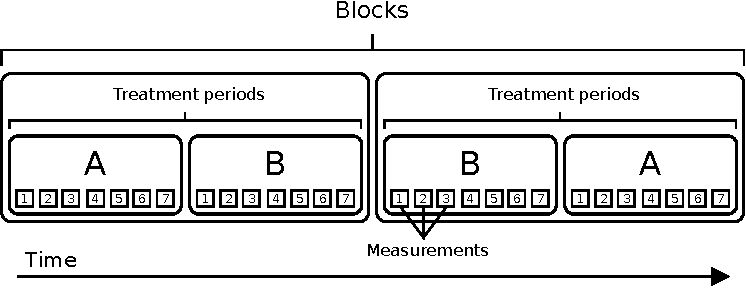
\includegraphics{design_for_simulated_experiment.pdf}
\end{figure}

\section{Simulating the Data}

Next, we simulate the data that we could get from our hypothetical experiment with Python.
As there should not be any interaction effects between the treatments, the treatment
effect onset is immediate and there is no washout period, this is a fairly simple
task. The benefit of having a relatively simple data generating process is that later it
is easier to compare the estimated results from our models with the actual parameters
values. We will not go over the code used to create the data in detail but concentrate on
the mathematical model that it is based on. The full code can be found in the GitHub repository
\cite{github}. For simulating each observation at time \(t\) for patient \(j\) we use the following model:

\begin{def}\label{simulationmodel}
    \begin{equation}\label{}
        y_{tj} = Z_{tj}\theta_{j} + W_{tj}\eta_{j} + t\beta_j + \epsilon_t + \rho_j\epsilon_{t-1},
    \end{equation}
\end{def}where \(\theta_j\) and \(\mu_j\) are the treatment effects with \(Z_{tj}\) and \(W_{tj}\) being indicator
variables that are 1 when observation \(t\) is within a period where treatment was applied and
0 otherwise. \(\beta_j\) is the trend representing the natural progress of the
condition. \(\epsilon_{tj} \sim N(0,\tau_j^2) \) is the error term at \(t\) and
\(\rho_j\) is the correlation between consecutive errors.

This data generating model has both a trend and a lag-1-autocorrelation. The trend we
are going to be modelling later, but also modelling autocorrelation would make the model
too complex for the limited amount observations we will be dealing with. This way the example tries to be more realistic
by having the data generating function to be of such complexity that it cannot be
fully modelled and some decisions have to be made on how to try to approximate
the process with a simplified version of reality.

``Above'' the part creating the individual observations we have population-level parameters
that define the distribution from which the patient-level parameters are drawn from.
Here we are mimicking a hierarchical model also in the data creation process. This is
important because if there was no underlying pattern to the patient-level parameter
values, pooling the information across the patients
would be nonsensical. So instead of directly picking the patient-level parameter values,
we are just going to pick the form of the distribution where these are drawn from.

\bigskip
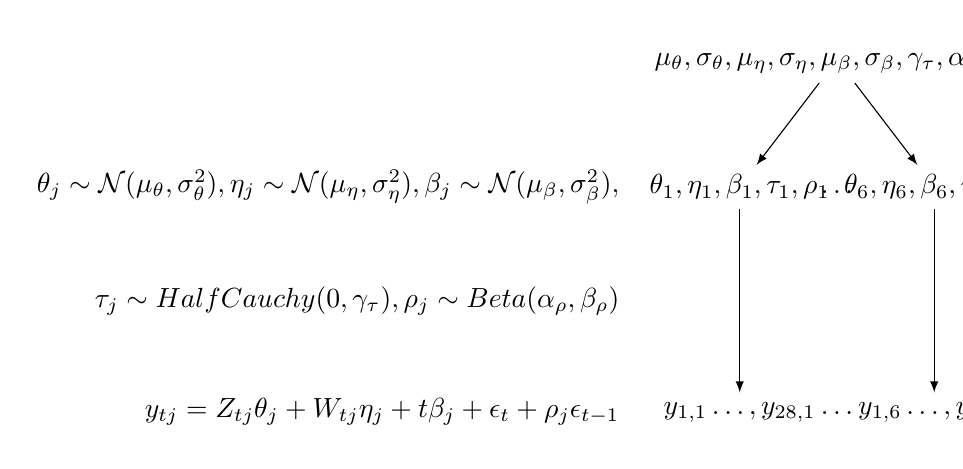
\begin{tikzpicture}

    \matrix[matrix of math nodes, column sep=-70pt, row sep=30pt] (mat)
    {
    \ & \mu_{\theta}, \sigma_{\theta}, \mu_{\eta},\sigma_{\eta}, \mu_{\beta},
    \sigma_{\beta}, \gamma_{\tau}, \alpha_{\rho}, \beta_{\rho} & \ \\
        \theta_1, \eta_1, \beta_1, \tau_1, \rho_1 & \ldots & \theta_6, \eta_6, \beta_6, \tau_6, \rho_6 & \\
        \ & \ & \ \\
        y_{1,1} \ldots, y_{28, 1} & \ldots & y_{1,6} \ldots, y_{28, 6} \\
    };

    \draw[->,>=latex] (mat-1-2) -- (mat-2-1);
    \draw[->,>=latex] (mat-1-2) -- (mat-2-3);
    \draw[->,>=latex] (mat-2-1) -- (mat-4-1);
    \draw[->,>=latex] (mat-2-3) -- (mat-4-3);

    \node[anchor=east] at ([xshift = -40pt]mat-2-1)
    {$
        \theta_j \sim \mathcal{N}(\mu_{\theta},\sigma_{\theta}^2),
        \eta_j \sim \mathcal{N}(\mu_{\eta},\sigma_{\eta}^2),
        \beta_j \sim \mathcal{N}(\mu_{\beta},\sigma_{\beta}^2),
    $};
    \node[anchor=east] at ([xshift = -40pt]mat-3-1)
    {$
        \tau_j \sim HalfCauchy(0, \gamma_{\tau}),
        \rho_j \sim Beta(\alpha_{\rho}, \beta_{\rho})
    $};
    \node[anchor=east] at ([xshift = -40pt]mat-4-1)
    {$
        y_{tj} = Z_{tj}\theta_{j} + W_{tj}\eta_{j} + t\beta_j + \epsilon_t + \rho_j\epsilon_{t-1}
    $};

\end{tikzpicture}
\bigskip

To create the simulated data, we set the population parameters to the values described
in table\ \ref{populationparameters} and then run
our data creation process:

\begin{table}[H]
    \caption{population-level Parameter Values for the Simulated Data}\label{populationparameters}
    \begin{align}\label{}
        \text{population treatment A mean: } & \mu_{\theta} = 10 \nonumber \\
        \text{population treatment A standard deviation: } & \sigma_{\theta} = 0.1 \nonumber \\
        \text{population treatment B mean: } & \mu_{\eta} = 9.6 \nonumber \\
        \text{population treatment B standard deviation: } & \sigma_{\eta} = 0.1 \nonumber \\
        \text{population trend mean: } & \mu_{\beta} = 0.02 \nonumber \\
        \text{population trend standard deviation: } & \sigma_{\beta} = 0.01 \nonumber \\
        \text{population measurement error scale: } & \gamma_{\tau} = 0.2 \nonumber \\
        \text{population error autocorrelation alpha: } & \alpha_{\rho} = 30 \nonumber \\
        \text{population error autocorrelation beta: } & \beta_{\rho} = 30 \nonumber
    \end{align}
\end{table}

There are some important things to note about these values. First, we defined the
treatment \(A\) to have a higher mean than treatment \(B\) and gave both of these a low
standard deviation meaning that the treatment \(B\) should perform better (lower
measurement values) for almost all patients.
Second, the mean of the trend \(\beta \) is positive and its variance is small. This means
that almost all patient should have a steadily worsening condition (measurements get
higher as the experiment progresses).

In figure\ \ref{measurementtimeline} we see timelines of the simulated measurements for
each patient. Just by looking, it seems
pretty obvious that for patient 6 there is a clear difference in the efficacy of the
treatments, with the treatment periods clearly visible as there is not much random
variation in the measurements. For other patients this not so
easy to tell as there is much more noise. Patient 2 stand out in this regard with
measurement values swinging wildly up and down.  We can also faintly see the upwards trend in the
measurements, with this being once again clearly noticeable for patient 6.

\begin{figure}[H]
    \caption{Timeline of Measurements for Each Patient}\label{measurementtimeline}
    \bigskip
    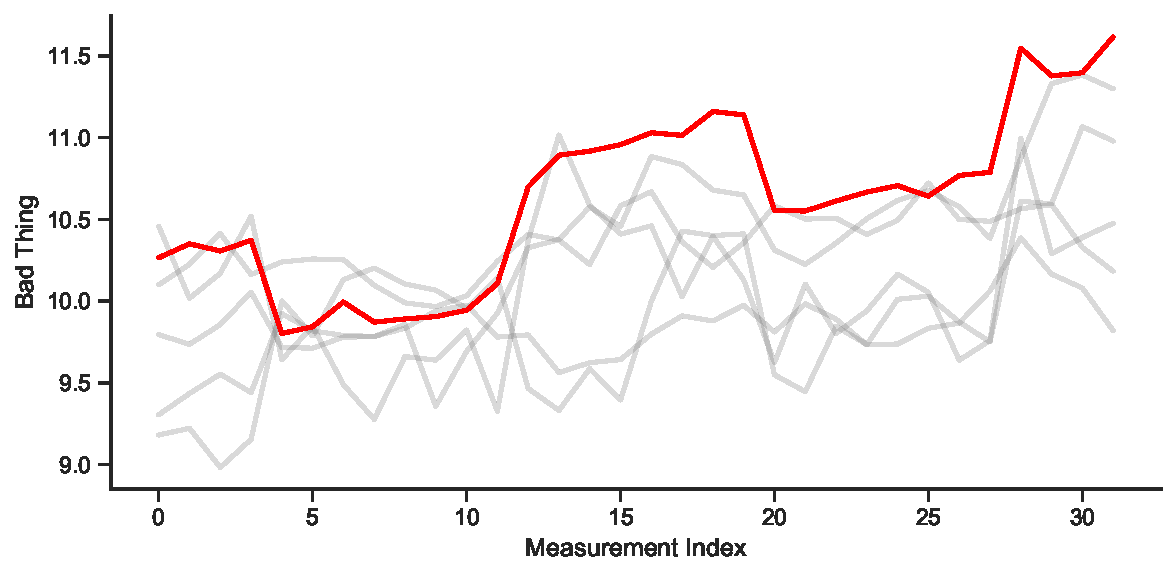
\includegraphics[width=\textwidth,height=\textheight,keepaspectratio]{measurements_timeline.pdf}
\end{figure}

Let's next look at the actual parameters that created this data.
In figure\ \ref{parameterdistribution}, we have all patient-level parameter values
overlaid on top of the population
distribution from which they were drawn from. On the left side we can see both of the
treatment effect means plotted on an identical x-axis for easy comparison.
We can see that for every patient treatment B is clearly
better (lower parameter values). The second interesting finding is that for patient
1 the treatment B effectiveness is far better than for other patients and the opposite
is true for patient 3. When we look later on at
the hierarchical model, these two patients are the ones to keep an eye out, as we would
expect the measurements from other patients to push the treatment effect of
treatment B for patient 1 up and conversely pull this down for patient
3. From the measurement error and autocorrelation, there are less interesting things to
note: the wild swings of the measurements for patient 2
are explained by her high measurement error, while patient 3 has almost exactly the same
measurement error, but also the highest autocorrelation, making her measurements less
erratic. For the trend we see patients split into two groups with patients 1, 5 and 6 getting
worse significantly faster than the others.

\begin{figure}[H]
    \caption{Parameter Used to Create Simulated Data}\label{parameterdistribution}
    \bigskip
    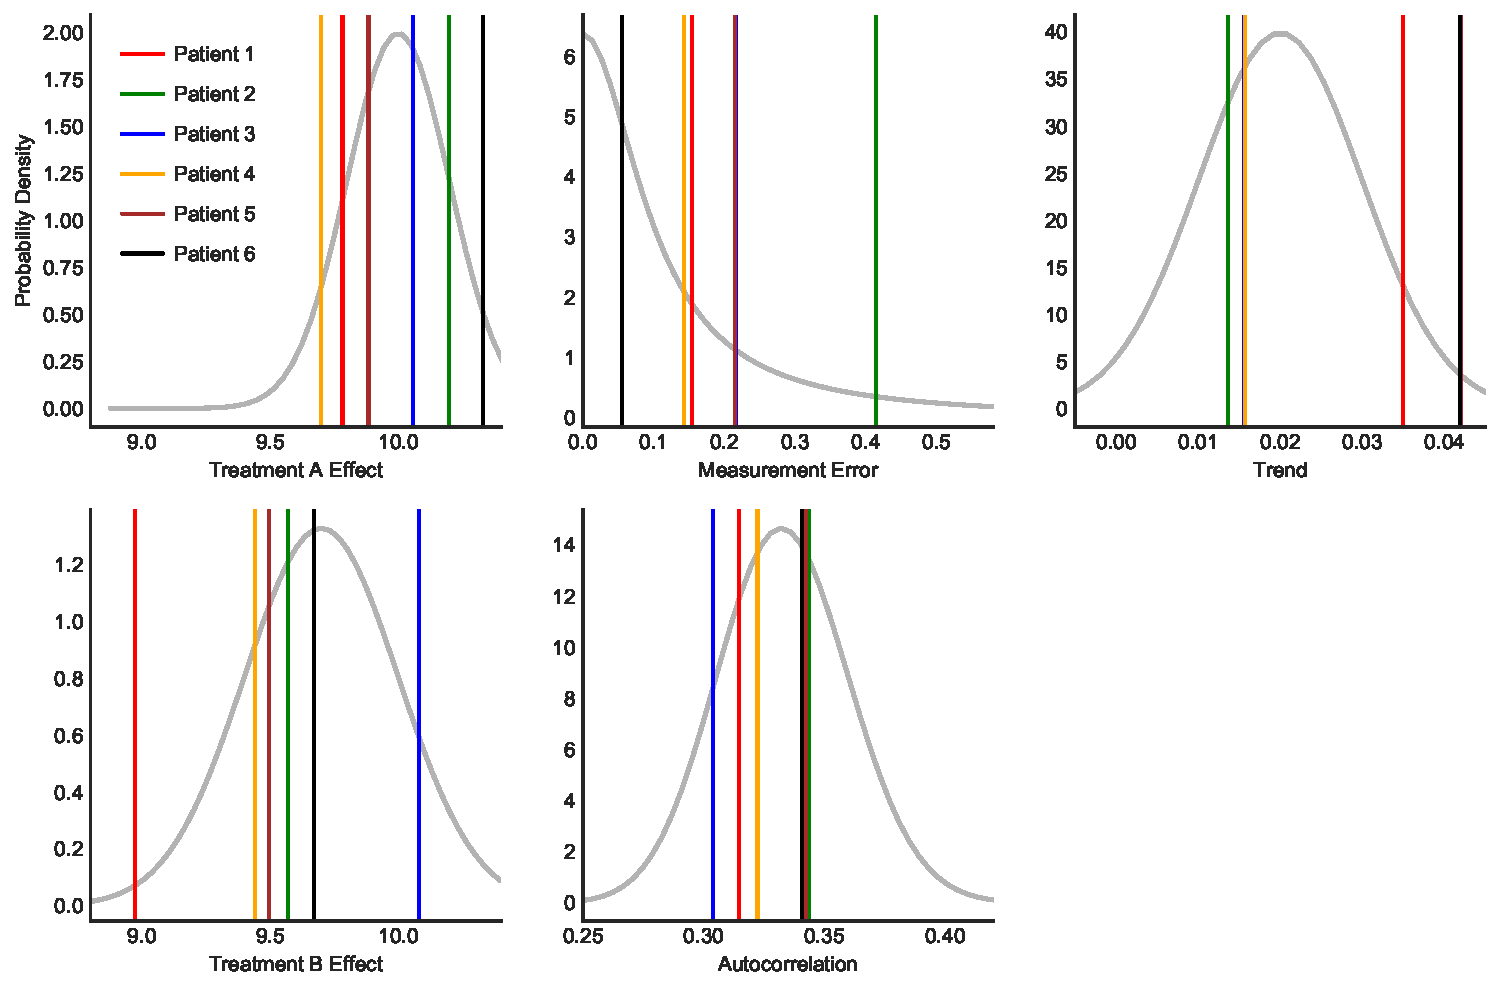
\includegraphics[width=\textwidth,height=\textheight,keepaspectratio]{population_parameter_distributions.pdf}
\end{figure}

\section{Analyzing a Single Trial}\label{1trial}

We start analyzing our simulated experiments by first focusing on just a single patient,
choosing naturally patient 1. In figure\ \ref{patient1timeline} we have the timeline of
observations for this patient. We have highlighted the period where the patient was on treatment A with grey and can
clearly see that this treatment seems to be the inferior option for this patient. With modelling
we should expect to get the same recommendation, but with more specificity.

\begin{figure}[H]
    \caption{Timeline of Measurements for Patient 1}\label{patient1timeline}
    \bigskip
    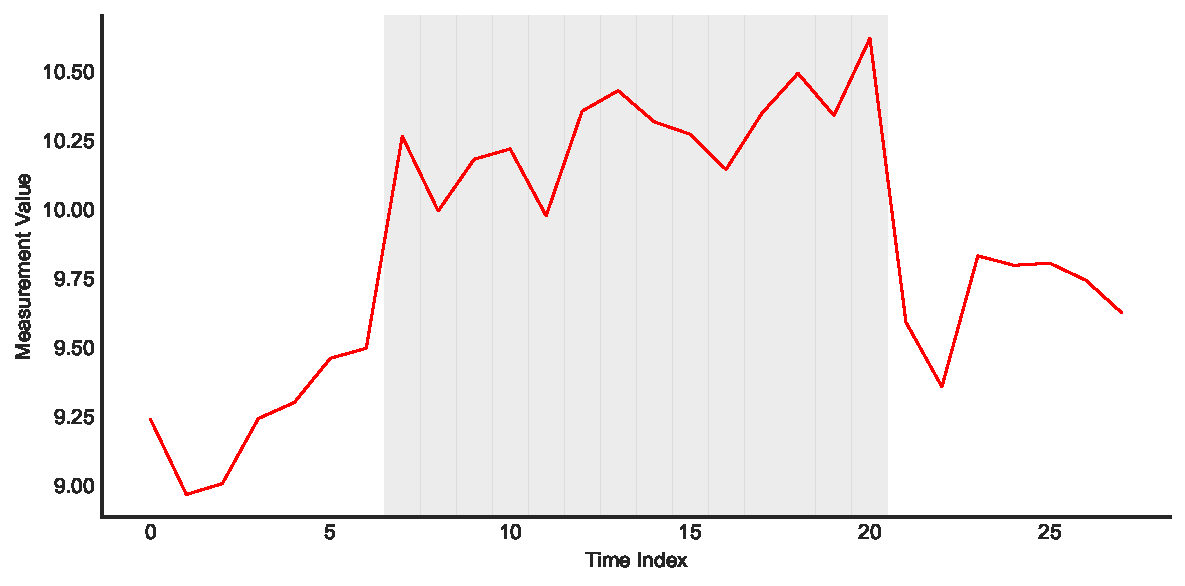
\includegraphics[width=\textwidth,height=\textheight,keepaspectratio]{patient1_timeline.pdf}
\end{figure}

Normally we would start with a more extensive exploration of the data, but as teaching preliminary analysis
is not the focus here and we have created the data ourself and so know exactly what kind
of distribution it follows and that there are no missing values or outliers, we will
skip this step here. For analyzing any real-world data, proper data exploration would be \emph{mandatory}.

\subsection{Defining the Model}

In our model we include the two treatment parameters, an error term and a trend\ (\ref{singlepatientmodel}). We could
start with a simpler model without the trend, but we know that there is a trend in
the data and we don't have the space to go deeper into model comparisons, so we start
with this more complicated model:

\begin{def}\label{}
    \begin{equation}\label{singlepatientmodel}
        y_t = Z_t\theta + W_t\eta + t\beta + \epsilon_t,
    \end{equation}
\end{def}where \(\theta \) and \(\eta \) are the treatment effects with \(Z_t\) and \(W_t\) being indicator
variables that are 1 when observation \(t\) is within a period where treatment was applied and
0 otherwise. \(\beta \) is the trend and \(\epsilon_{t} \sim N(0,\tau^2) \) is the error term at \(t\).

Our model assumes that the measurement values are distributed normally with
variance \(\tau^2\) and a mean of either \(\theta \) or \(\eta \) depending on which
treatment is applied during the observation \(y_t \sim N(Z_t\theta + W_t\eta, \tau^2)\).
This means that our likelihood function will have to be a bit special as using a simple
normal distribution will not do. We will see that this will cause us some headaches
later when we implement the model in PyMC3.

Next, we go to choose the prior distributions for our model. We choose a
normal distributions for the treatment effects and the trend as it makes sense to think
that these would depend on multiple independent biological and social
factors and the central limit theorem tells us the that
the parameters should then be normally distributed. For the variance of the error
term we choose a half-Cauchy distribution as this is a common recommendation for the
prior of variance when we have some prior information\ \cite{variancepriors}.

\bigskip
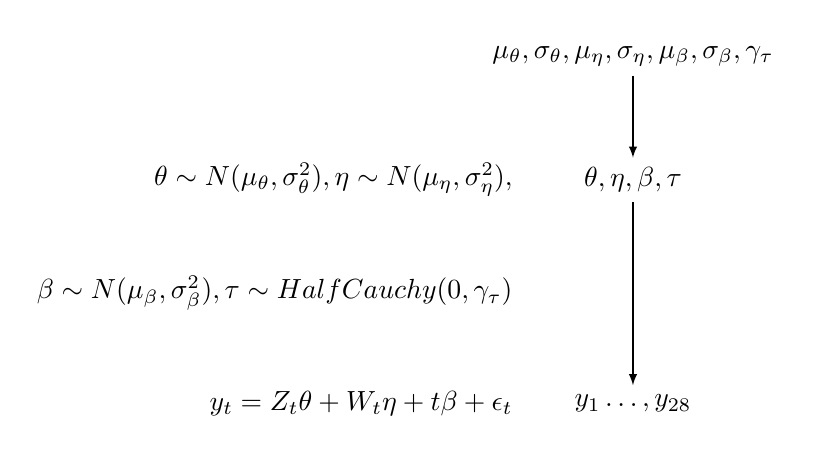
\begin{tikzpicture}

    \matrix[matrix of math nodes, column sep=0pt, row sep=30pt] (mat)
    {
        \mu_{\theta}, \sigma_{\theta}, \mu_{\eta}, \sigma_{\eta}, \mu_{\beta}, \sigma_{\beta}, \gamma_{\tau} \\
        \theta, \eta, \beta, \tau \\
        \ \\
        y_{1} \ldots, y_{28} \\
    };

    \draw[->,>=latex] (mat-1-1) -- (mat-2-1);
    \draw[->,>=latex] (mat-2-1) -- (mat-4-1);

    \node[anchor=east] at ([xshift = -40pt]mat-2-1)
    {$
        \theta \sim N(\mu_{\theta}, \sigma^2_{\theta}),
        \eta \sim N(\mu_{\eta}, \sigma^2_{\eta}),
    $};
    \node[anchor=east] at ([xshift = -40pt]mat-3-1)
    {$
        \beta \sim N(\mu_{\beta}, \sigma^2_{\beta}),
        \tau \sim HalfCauchy(0, \gamma_{\tau})
    $};
    \node[anchor=east] at ([xshift = -40pt]mat-4-1)
    {$
        y_t = Z_t\theta + W_t\eta + t\beta + \epsilon_t
    $};

\end{tikzpicture}
\bigskip

Now that we have our model defined we should think about what kind of values we should
give to our prior parameters. Let's say there exists a prior study with 25 participants
that evaluated the same treatments. The obvious priors for the treatment effects means
are the means calculated from this previous study, this number being (hypothetically) 10 for both
treatments. The same method can be applied to get the prior for the mean of the trend. For
the standard deviations of treatment effects and trend, we can use the standard deviation
of the patient treatment and trend means for the patients from the existing study. As we
are not sure how representative patients in the previous study were of our patients, we
can broaden the standard deviations to reflect this by multiplying them by 2. The values
we get this way are 3 for both of the treatment effect standard deviations and 0.8 for
the trend. As the scale of the half-Cauchy
distribution is the median of the distribution, we can use the median of
the standard deviation of the existing patient-level measurements after a similar model that we
are using is fitted to the data. Once again we should broaden this number to reflect our uncertainty of the
applicability of the prior studies, so we double this number from 0.5 to 1.
The chosen prior values can be seen in table\ \ref{singlelpatientmodelpriorvalues}.

\begin{table}[H]
    \caption{Single Patient Model Prior Values}\label{singlelpatientmodelpriorvalues}
    \begin{align}\label{}
        \text{treatment A mean prior: } & \mu_{\theta} = 10 \nonumber \\
        \text{treatment A standard deviance prior: } & \sigma_{\theta} = 3 \nonumber \\
        \text{treatment B mean prior: } & \mu_{\eta} = 10 \nonumber \\
        \text{treatment B standard deviance prior: } & \sigma_{\eta} = 3 \nonumber \\
        \text{trend mean prior: } & \mu_{\beta} = 0.2 \nonumber \\
        \text{trend standard deviance prior: } & \sigma_{\beta} = 0.8 \nonumber \\
        \text{measurement error scale prior: } & \gamma_{\tau} = 1 \nonumber
    \end{align}
\end{table}

\subsection{Implementing the Model}

PyMC3 is Python package built for probabilistic programming. Although it is not
limited to Bayesian methods, that is its main focus. Implementing Bayesian models in
the package works so that you give it all the parts of the Bayesian formula except the
marginal likelihood: the likelihood, prior
distribution and the values defining the prior distributions. It uses the NUTS
sampler\cite{nuts} to algorithmically approximate the posterior distribution. This is
very nice, as this takes out a huge chunk of work from us, namely choosing and
implementing the approximation method
ourself. But now that we have entered the territory of algorithmic solutions, we have
introduced a new hurdle, namely checking that the algorithm works for our
model and gives us good approximations. On top of this, we should check that our model is a good
approximation of reality. We will go over how  we can deal with them when they pop up, so let's just jump in and
implement the model in PyMC3 and afterwards walk through what the code is
doing line by line\footnote{The code snippets shown are a
slight simplification of the actual code that was used. This does not mean
that the code shown is not executable, but parts of it that are related to technical niceties
(e.g.\ inter-OS compatibility, saving the plots) are taken out to focus on what is
important.}.

\pagebreak

\subsubsection*{Full Model Implementation in PyMC3}
\bigskip
\begin{pyverbatim}[][fontsize=\footnotesize]
# load in needed packages
import pymc3 as pm
import pandas as pd

# read measurement data and the true parameter values
measurements_df = pd.read_csv("patient_measurements.csv")
parameters_df = pd.read_csv("patient_parameters.csv")

# create convenience index for easy filtering
patient_idx = measurements_df["patient"]
   
# define the model
with pm.Model() as single_patient_model:

    # defining our prior beliefs of the distributions of parameters
    treatment_a = pm.Normal("Treatment A", mu=10, sigma=3)
    treatment_b = pm.Normal("Treatment B", mu=10, sigma=3)
    trend = pm.Normal("Trend", mu=0.1, sigma=0.8)
    gamma = pm.HalfCauchy("Gamma", beta=1)

    # creating a vector defining the expected means of the observations
    # which are defined by one of the treatment means + trend
    measurement_means = (
        treatment_a * measurements_df[patient_idx == 0]["treatment_a"]
        + treatment_b * measurements_df[patient_idx == 0]["treatment_b"]
        + trend * measurements_df[patient_idx == 0]["measurement"]
    )

    # likelihood is multivariate normal distribution with the same amount of dimensions
    # as the patient has measurements with means defined by the previously
    # defined vector and all dimensions share the same variance
    likelihood = pm.Normal(
        "y",
        measurement_means,
        sigma=gamma,
        observed=measurements_df[patient_idx == 0]["value"],
    )

    # adding the comparison between the treatments for monitoring
    difference = pm.Deterministic(
        "Treatment Difference (A-B)", treatment_a - treatment_b
    )

    # running the algorithmic estimation process
    trace = pm.sample(draws=1000, tune=600, cores=3)

    # Checking diagnostic describing how the algorithm performed
    pm.traceplot(
        trace, var_names=["Treatment A", "Treatment B", "Trend", "Gamma"]
    )
    plt.show()
    pm.summary(trace, kind="diagnostics")

    # checking the posterior distributions
    pm.plot_posterior(trace, credible_interval=0.95)
    plt.show()

 
# creating new observations based on our model with sampled
# posterior estimates (posterior sampling)
with single_patient_no_trend_model as model:
    post_pred = pm.sample_posterior_predictive(trace, samples=500)
    predictions = post_pred["y"]

# visualizing posterior samples to check the model's match with reality
draw_posterior_checks(
    predictions=predictions,
    measurements_df=measurements_df[patient_idx == 0],
    parameters_df=parameters_df[parameters_df["patient"] == 0],
)
\end{pyverbatim}
\smallskip

\subsubsection*{Part 1: Loading in the Package and the Data}

\bigskip
\begin{pyverbatim}[][fontsize=\footnotesize]
import pymc3 as pm
import pandas as pd

measurements_df = pd.read_csv("patient_measurements.csv")
parameters_df = pd.read_csv("patient_parameters.csv")

patient_idx = measurements_df["patient"]
\end{pyverbatim}
\smallskip

The first thing we of course have to do is to load the required packages and get our data. There is
not much to comment about loading the packages, but let's see how our data in
\pyv{measurements_df} looks like:

\bigskip
\begin{table}[H]
\caption{Structure of the Measurement Data}\label{measurements}
\bigskip
\centering
\begin{pycode}
import os
import pandas as pd

measurements_path = os.path.join("..", "data", "patient_measurements.csv")
measurements_df = pd.read_csv(measurements_path)
measurements_df.columns = ['patient', 'measurement', 'period', 'block',
'treatment_a', 'treatment_b', 'value']
print(measurements_df.head(10).to_latex(index=False))
\end{pycode}
\end{table}
\bigskip

All columns except the last one are index columns. As is the standard in Python, everything
zero-indexed. The first column indexes the patient (0--5), second the
measurement (0-27), third the treatment period (0--3), fourth the block (0--1) and fifth
and sixth which treatment was applied during the particular measurement (0--1). The last
column contains the values of the measurements. This format was chosen just for
convenience as PyMC3 does not require any particular format as long as you can feed the right values into
the right places in the model definition. Also using the pandas package to handle the
data as a dataframe is not necessary, but is very convenient.

The \pyv{parameters_df} dataframe shown in table\ \ref{parameters} contains the true
parameter values of the patients. These can be used to check how accurate our predictions
are. With real-world data, we would
not have access to these values, but as we created the data ourself, we do and we should
take advantage of that. Each row in this dataset is a patient and contains the
true parameter values for each of the parameters we used to create the simulated data.
Only a couple of the columns included in the dataset are shown here because the full
table would not fit.

\bigskip
\begin{table}[H]
\caption{Structure of the Parameter Data}\label{parameters}
\bigskip
\centering
\begin{pycode}
import os
import pandas as pd

parameters_path = os.path.join("..", "data", "patient_parameters.csv")
parameters_df = pd.read_csv(parameters_path)
parameters_df.drop(columns=["treatment_order", 'autocorrelation'], inplace=True)
parameters_df.columns = ['patient', 'treatment_a', 'treatment_b', 'trend', 'measurement_error_sd']
print(parameters_df.to_latex(index=False))
\end{pycode}
\end{table}
\smallskip

The last part of the code where we create the variable \pyv{patient_idx} is just for
convenience so that we need to type less when referring to the data of a particular patient.

\subsubsection*{Part 2: Initializing the Model}

\bigskip
\begin{pyverbatim}[][fontsize=\footnotesize]
with pm.Model() as single_patient_model:
\end{pyverbatim}
\smallskip

PyMC3 models are usually defined within the Python context manager (``with'' statements).
This is not necessary but makes the model definition much cleaner as all parts
defined within the context (indented parts of the code), are automatically associated
with the model without the need to manually define this.

\subsubsection*{Part 3: Defining the Priors}

\bigskip
\begin{pyverbatim}[][fontsize=\footnotesize]
    treatment_a = pm.Normal("Treatment A", mu=10, sigma=3)
    treatment_b = pm.Normal("Treatment B", mu=10, sigma=3)
    trend = pm.Normal("Trend", mu=0.1, sigma=0.8)
    gamma = pm.HalfCauchy("Gamma", beta=1)
\end{pyverbatim}
\smallskip

Now we start getting to the actual modelling. We start by defining our prior beliefs about
the parameter distributions. For both of the treatments and the trend, we use a normal distribution and
for the variance of the error term \(\gamma \) we use a half-Cauchy. For the half-Cauchy
distribution we don't need to define the location term as it is by default zero.
Something to note here is that the PyMC3 normal distribution sigma
parameter takes in the standard deviation and not the variance. As all the distributions
that we are using here are common and well defined, we can find inbuilt functions implementing
them already in PyMC3. It is also possible to define completely custom
distributions, but unfortunately this is quite complex, as you don't just have to worry
about the mathematical part, but also all you have to implement all the helper methods that PyMC3
relies on\footnote{Because of the complexity of defining
custom distributions the author would recommend using the competing PyStan package in
cases where inbuilt distributions don't exist. Although Stan requires you to write
model definition with its own language, this hurdle is worth it in most some cases as you can focus
more on the mathematical side without the need to consider replicating poorly documented helper methods}.

\subsubsection*{Part 4: Defining the Likelihood}

\bigskip
\begin{pyverbatim}[][fontsize=\footnotesize]
    measurement_means = (
        treatment_a
        * measurements_df[patient_idx == 0]["treatment_a"]
        + treatment_b
        * measurements_df[patient_idx == 0]["treatment_b"]
        + trend
        * measurements_df[patient_idx == 0]["measurement"]
    )

    likelihood = pm.Normal(
        "y",
        measurement_means,
        sigma=gamma,
        observed=measurements_df[patient_idx == 0]["value"],
    )
\end{pyverbatim}
\smallskip

Defining the likelihood is the most difficult part of our model definition because of the
complexity introduced by the varying treatments. Because of this, the likelihood cannot
be implemented as a simple normal distribution. We solve this problem by instead using a
multivariate normal distribution with as many dimensions as the patient has
measurements. We construct the vector of means for this distribution by multiplying the
treatment distributions by the treatment indicators (1 when
treatment is given, 0 when not) and add the trend multiplied by the index of the
measurement (\(t\)). So instead of considering
the observations as multiple samples from the same distribution, we think of them as a
single multidimensional sample from
a multivariate normal distribution. The key here is that every measurement will give
information about only of the treatment parameters as the indicator value sets the
value to zero for the treatment that was not administered during the
measurement that the dimension is representing. This is not the only possible way to solve the
problem but is probably the most convenient. If we would have some
dependencies between the measurements in our model (e.g.\ due to autocorrelation), this approach
would not work. In this case, we would have to implement the likelihood function
ourselves.

One technical detail to note here is that even though we are using a multivariate normal
distribution we still use the same PyMC3 function for normal distribution and just give
it a vector of means that matches the number of our observations. This strategy works
with all the inbuilt PyMC3 distributions: you can either have them use a single
parameter value or a vector of values matching the dimensions of the data and PyMC3 will automatically
change from using a single-dimensional distribution with multiple observations to
multidimensional distribution with one observation.

\subsubsection*{Part 5: Defining the Parameter Comparison}

\bigskip
\begin{pyverbatim}[][fontsize=\footnotesize]
    difference = pm.Deterministic(
        "Treatment Difference (A-B)", treatment_a - treatment_b
    )
\end{pyverbatim}
\smallskip

As the estimate we are most interested is not any individual parameter, but the
difference between the two treatment parameters, we have to add this comparison separately.
We can do this before or after running our model, but here we have decided to do it
beforehand. As the difference is fully determined by the values of the treatment
parameters we have to use PyMC3s
\pyv{pm.deterministic} function and calculate the posterior
by simply subtracting the value of treatment 2 parameter value from treatment 1
parameter value after sample from the posterior. This makes sure that the possible
dependencies between these parameters are taken into account.

\subsubsection*{Part 6: Running the Model}

\bigskip
\begin{pyverbatim}[][fontsize=\footnotesize]
    trace = pm.sample(draw=1000, tune=600, cores=3)
\end{pyverbatim}
\smallskip

Now that we have defined our prior beliefs and our likelihood, we can move on to running the
model. PyMC3 will now estimate the posterior with the NUTS sampler,
that samples the distribution defined by likelihood times priors and estimates the
posterior based on these samples. If we want to manually tune the sampling parameters or
use a completely different sampling method, PyMC3 offers a wide range of options, but
unless we see problems when we evaluate the estimation efficiency,
we should stick with the default options. The three parameters that we have to manually define are as follow:

\begin{itemize}
    \item[] draw = how many steps the chain should calculate
    \item[] tune = how many steps the chain should take before it starts to
    take the observations into account
    \item[] cores = how many chains to calculate in parallel
\end{itemize}

The total steps taken by each chain is draw+tune. The reason for the tuning steps is
that the starting position of the chain is probably biased. We would want the starting
position to be equivalent to a random sample from the posterior. We can do this by letting the chain first take
a number of steps and as its moves through the posterior its location distribution will start to
reflect the actual posterior. If we would not have the tuning steps it would be possible
to have the chain starts in a weird position and the first steps it takes don't reflect the
posterior as it might have to make lots of moves in a certain direction to get to the
representative parts of the distribution. In principle, we could use the tuning steps
for the calculation as long as we have enough steps as the product would
still eventually converge to the same distribution, but it is more efficient to just drop these
values so that we don't have to add more steps to compensate the possible bias introduced by
them. The more draws and tuning steps we take the better the estimation will be, but the
more time the calculation will take. Finding the
right number of draw and tuning steps involves usually some trial and error. It is
hard to know how many steps you need before you try to run the model. Luckily PyMC3 will
automatically alert us if it thinks that we need more tuning steps or draws and we can
also diagnose this from the metrics and plots that we will look at after we have run the
model.

As modern CPUs have usually multiple cores, we can speed up the calculation by running
multiple chains in parallel. Each chain is independent of each other and will
take the same amount of draws and tuning steps. As the chains can run in parallel, having
multiple chains running can dramatically speed up our estimation. The total number of steps that
the posterior will be calculated with is the combined draws (not tuning steps) of the
chains. So in our case, we will use 3 cores and have 3 chains (running this on a 4 core
CPU so we will leave 1 core free for other tasks), these chains will make in total (1000 +
600) * 3 = 4800 steps, of which 1000 * 3 = 3000 steps will be used for the posterior estimation.

\subsubsection*{Part 7: Checking Algorithm Diagnostics}

\bigskip
\begin{pyverbatim}[][fontsize=\footnotesize]
    pm.traceplot(
            trace, var_names=["Treatment A", "Treatment B", "Trend", "Gamma"]
        )
    plt.show()
    pm.summary(trace)
\end{pyverbatim}
\smallskip

Now that we have run the model we need to evaluate if the algorithm did a good job with
the estimation. We can get a sense of this by looking at diagnostic plots and metrics.
Let's first look at the visualizations of the chain steps called traceplots:

\begin{figure}[H]
    \caption{Single Patient Traceplots}\label{traceplots}
    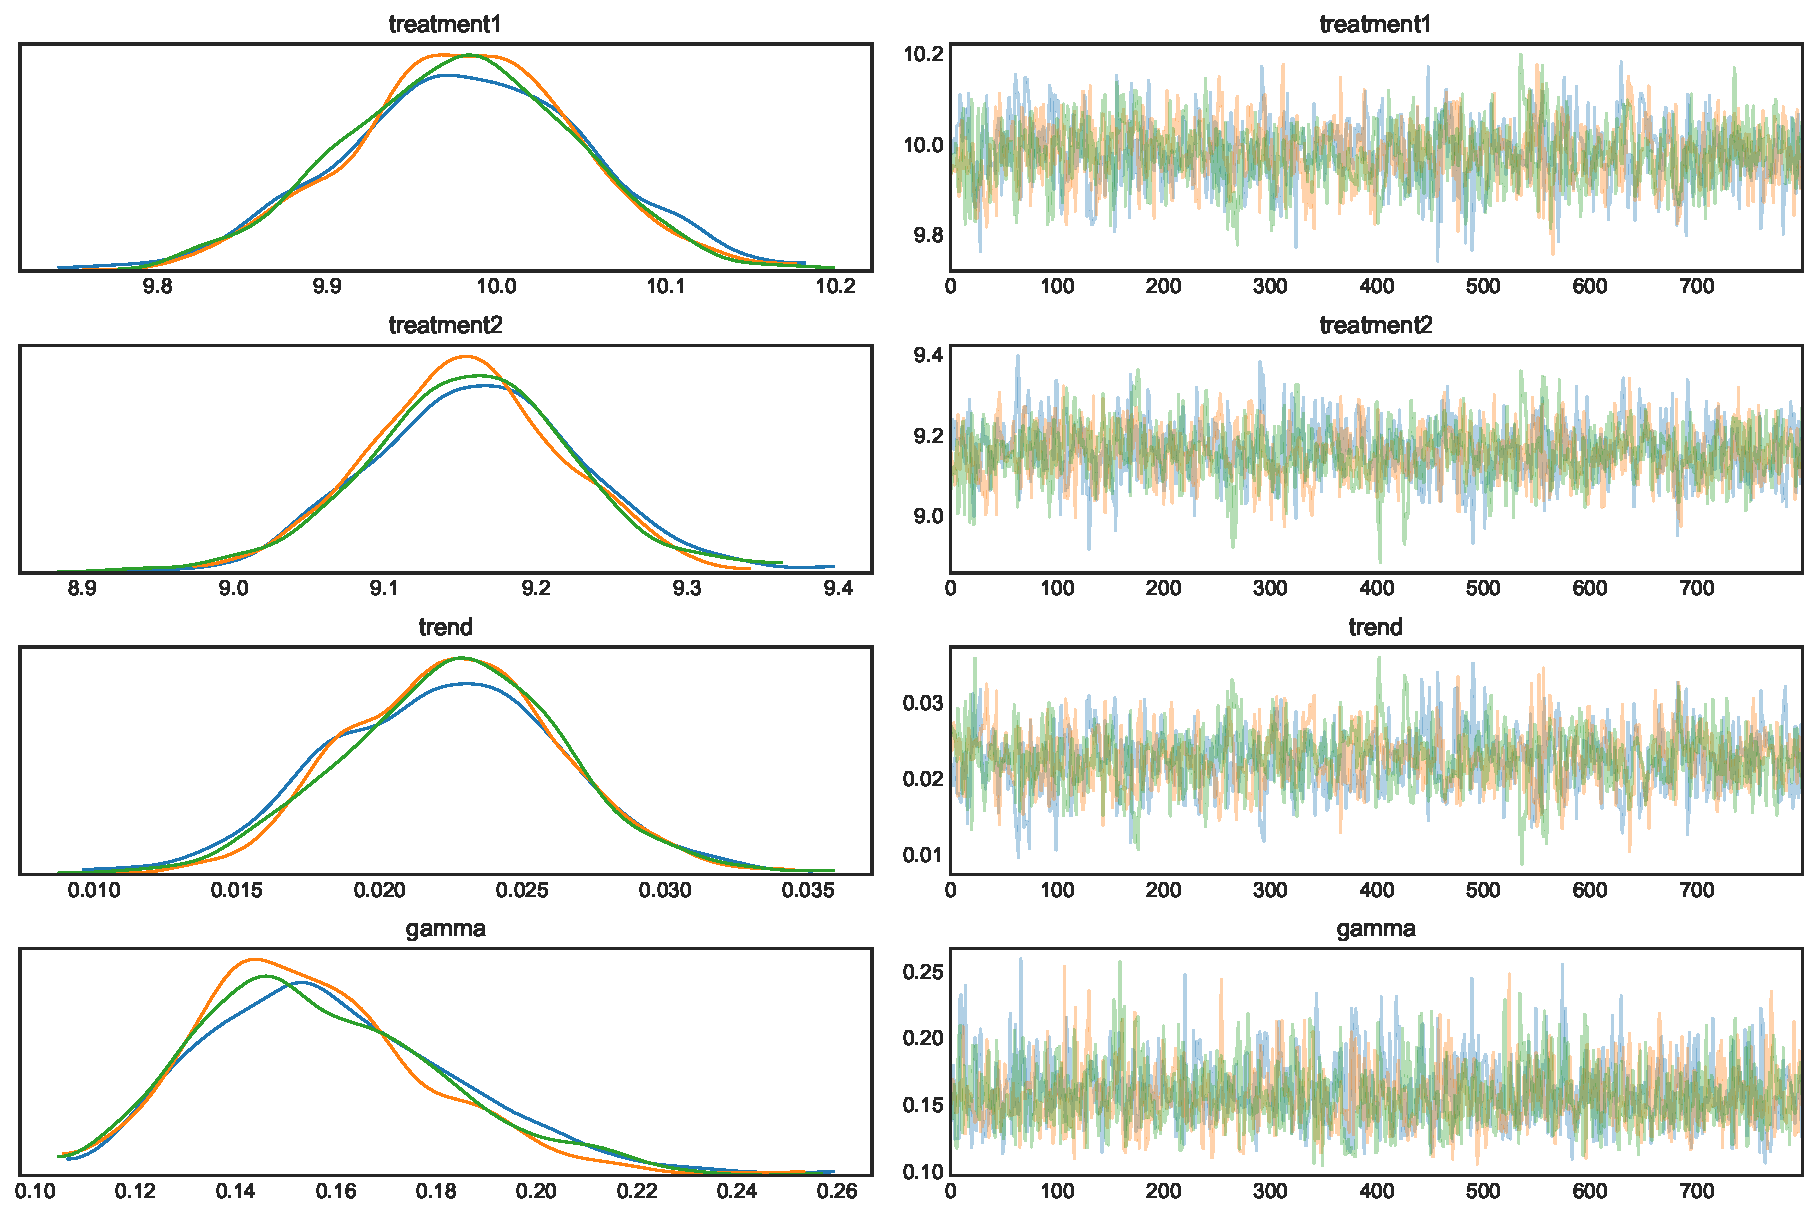
\includegraphics[width=\textwidth,height=\textheight,keepaspectratio]{single_patient_traceplot.pdf}
\end{figure}

On the right side in figure\ \ref{traceplots} we can see the timeline of the values of the
four parameters in the steps taken by each of our
chains (remember from Chapter\ \ref{bayesinferencechallenges} that
each chain always evaluates all parameters). These are just the steps used for the
posterior estimation and don't include the
tuning steps. Each chain is portrayed in a different colour. What we want to see
here is that the timelines look like random noise around a single value with no obvious
patterns. If our distributions would be multimodal we would expect to see noise around
multiple values with frequent jumps from one mode to another. The things
we don't want to see are value drift or chains getting stuck into one area of the
distribution. If we would see something like this,
it would mean that the chains had problems moving through the posterior and ended up
taking biased samples. These effects should be most pronounced at the beginning
steps and if we would see these, we should increase the number of tuning
steps.

On the left side of the figure, we can see the distribution of the sampled values for
each chain. Here we would want to see that distributions from different chains more or
less align with
each other. If this is not the case, it means that the chains got stuck in different
parts of the posterior or our tuning steps were not enough to diminish the effect of
different starting points. This issue would also show on the left side plots with the different
chains staying in different parts of the posterior or being distinguishable from each
other. If we see this problem the solution is once again to increase the tuning steps.

Besides looking at plots, we can also estimate the success of the estimation from
diagnostic metrics. PyMC3 has an inbuilt method for printing the common metrics
(\pyv{pm.summary(trace)}). Below in table\ \ref{singlepatientdiagnosticmetrics} we can see the output
of this method for two of the main metrics (the full output is too big to display here):

\bigskip
\begin{table}[H]
    \caption{Single Patient Model Diagnostic Metrics}\label{singlepatientdiagnosticmetrics}
    \bigskip
    \centering
    \begin{tabular}{lrrrrrrr}
\toprule
{} &  mcse\_mean &  mcse\_sd &  ess\_mean &  ess\_sd &  ess\_bulk &  ess\_tail &  r\_hat \\
\midrule
treatment1 &      0.002 &    0.002 &     904.0 &   904.0 &     905.0 &    1094.0 &    1.0 \\
treatment2 &      0.002 &    0.002 &     895.0 &   895.0 &     898.0 &    1105.0 &    1.0 \\
trend      &      0.000 &    0.000 &     848.0 &   829.0 &     850.0 &    1023.0 &    1.0 \\
gamma      &      0.001 &    0.000 &    1209.0 &  1175.0 &    1275.0 &    1207.0 &    1.0 \\
\bottomrule
\end{tabular}

\end{table}
\smallskip

The metrics displayed in the table are effective sample size metrics (\pyv{ess_*})
and potential scale reduction statistic \(\hat{R}\) (\pyv{r_hat}). The effective sample
size metrics describe how many independent draws from the posterior our calculated steps
represent. The more autocorrelation there is between the draws, the less effective the
sampling is. As the autocorrelation affects the estimation of different parameters
differently the metric has multiple variants. \pyv{ess_bulk} tries to be a
diagnostic estimating the effectiveness of the sampling in general\cite{essbulk},
while \pyv{ess_mean} is for estimation the mean and
\pyv{ess_tail} for estimating the 5 \% and 95 \% quantiles. We can see that with all
of these variants our sample is quite large but considerably smaller than the 2400
steps we took. The \(\hat{R}\)-metric
tells us if the chains have converged to an equilibrium distribution. The metric is calculated by
taking the variance of the drawn values for each chain,
then calculating the variance of drawn values for all chains combined and then taking the
ratio of the average of the per chain variance compared to the pooled variance. If the
chains have converged to a common distribution the value of this metric will be one. If
the value is higher than one, this indicates that the chains have not converged. Small
divergences between the chains are not critical and \(\hat{R}\) values less than 1.1 should
not give cause for concern\ \cite{rhatrule}. In our case \(\hat{R}\) values are at 1.0 for
all metrics, so everything seems to be in order.

If we find problems in the traceplots and diagnostic metrics and increasing the tuning
steps does not seem to help, we have two options: modifying the MCMC algorithm
parameters or reparametrizing our model. There are lots of ways to tune the
default NUTS sampler used by PyMC3. If increasing the tuning steps seems to help with
the model getting better but too slowly, you could change the initialization method, that
defines how the start location is chosen and how
the chain starts moving initially before it gets a better estimate of the shape of the
posterior. This might make the start locations more representative of the posterior and
also make the initial movements of the chain better, decreasing the time that the chains
need to converge to the posterior distribution. We could also try to increase the
parameter \pyv{target_accept} that defines the target acceptance rate for the steps
that the chains take. Increasing this value from the default 0.8 to 0.9 or 0.95 makes the
steps smaller and increases autocorrelation, but lessens the change that chains get
stuck. If this does not help, we
can think about reparametrizing our model. We could change the distributions and prior
values used, simplify our model by getting rid of possible unimportant variables and making
some variables deterministic by estimating their value straight from the data (e.g.
variance). There is also the third option: we could change the MCMC algorithm used. This
rarely the right choice as the NUTS sampler is superior to the older samplers in almost
every situation\footnote{PyMC3 also support variational
inference which is even more effective than NUTS, but it is only for calculating approximate
solutions.}.

One thing that we should note here is that we only looked at diagnostic values for our
parameters, but not the difference between the treatment means which we are actually
most interested in. The reason for this is that the difference is entirely determined
by the individual treatment parameters, so if the estimation of these is in order, so
will be the estimate of their difference.

\subsubsection*{Part 8: Checking the Posterior}

\bigskip
\begin{pyverbatim}[][fontsize=\footnotesize]
    pm.plot_posterior(trace, credible_interval=0.95)
\end{pyverbatim}
\smallskip

If the estimation looks fine, we can move on to checking the actual results and look at
the computed posterior distributions shown in figure\ \ref{singlepatientposteriors}:

\bigskip
\begin{figure}[H]
    \caption{Single Patient Posterior Distributions}\label{singlepatientposteriors}
    \bigskip
    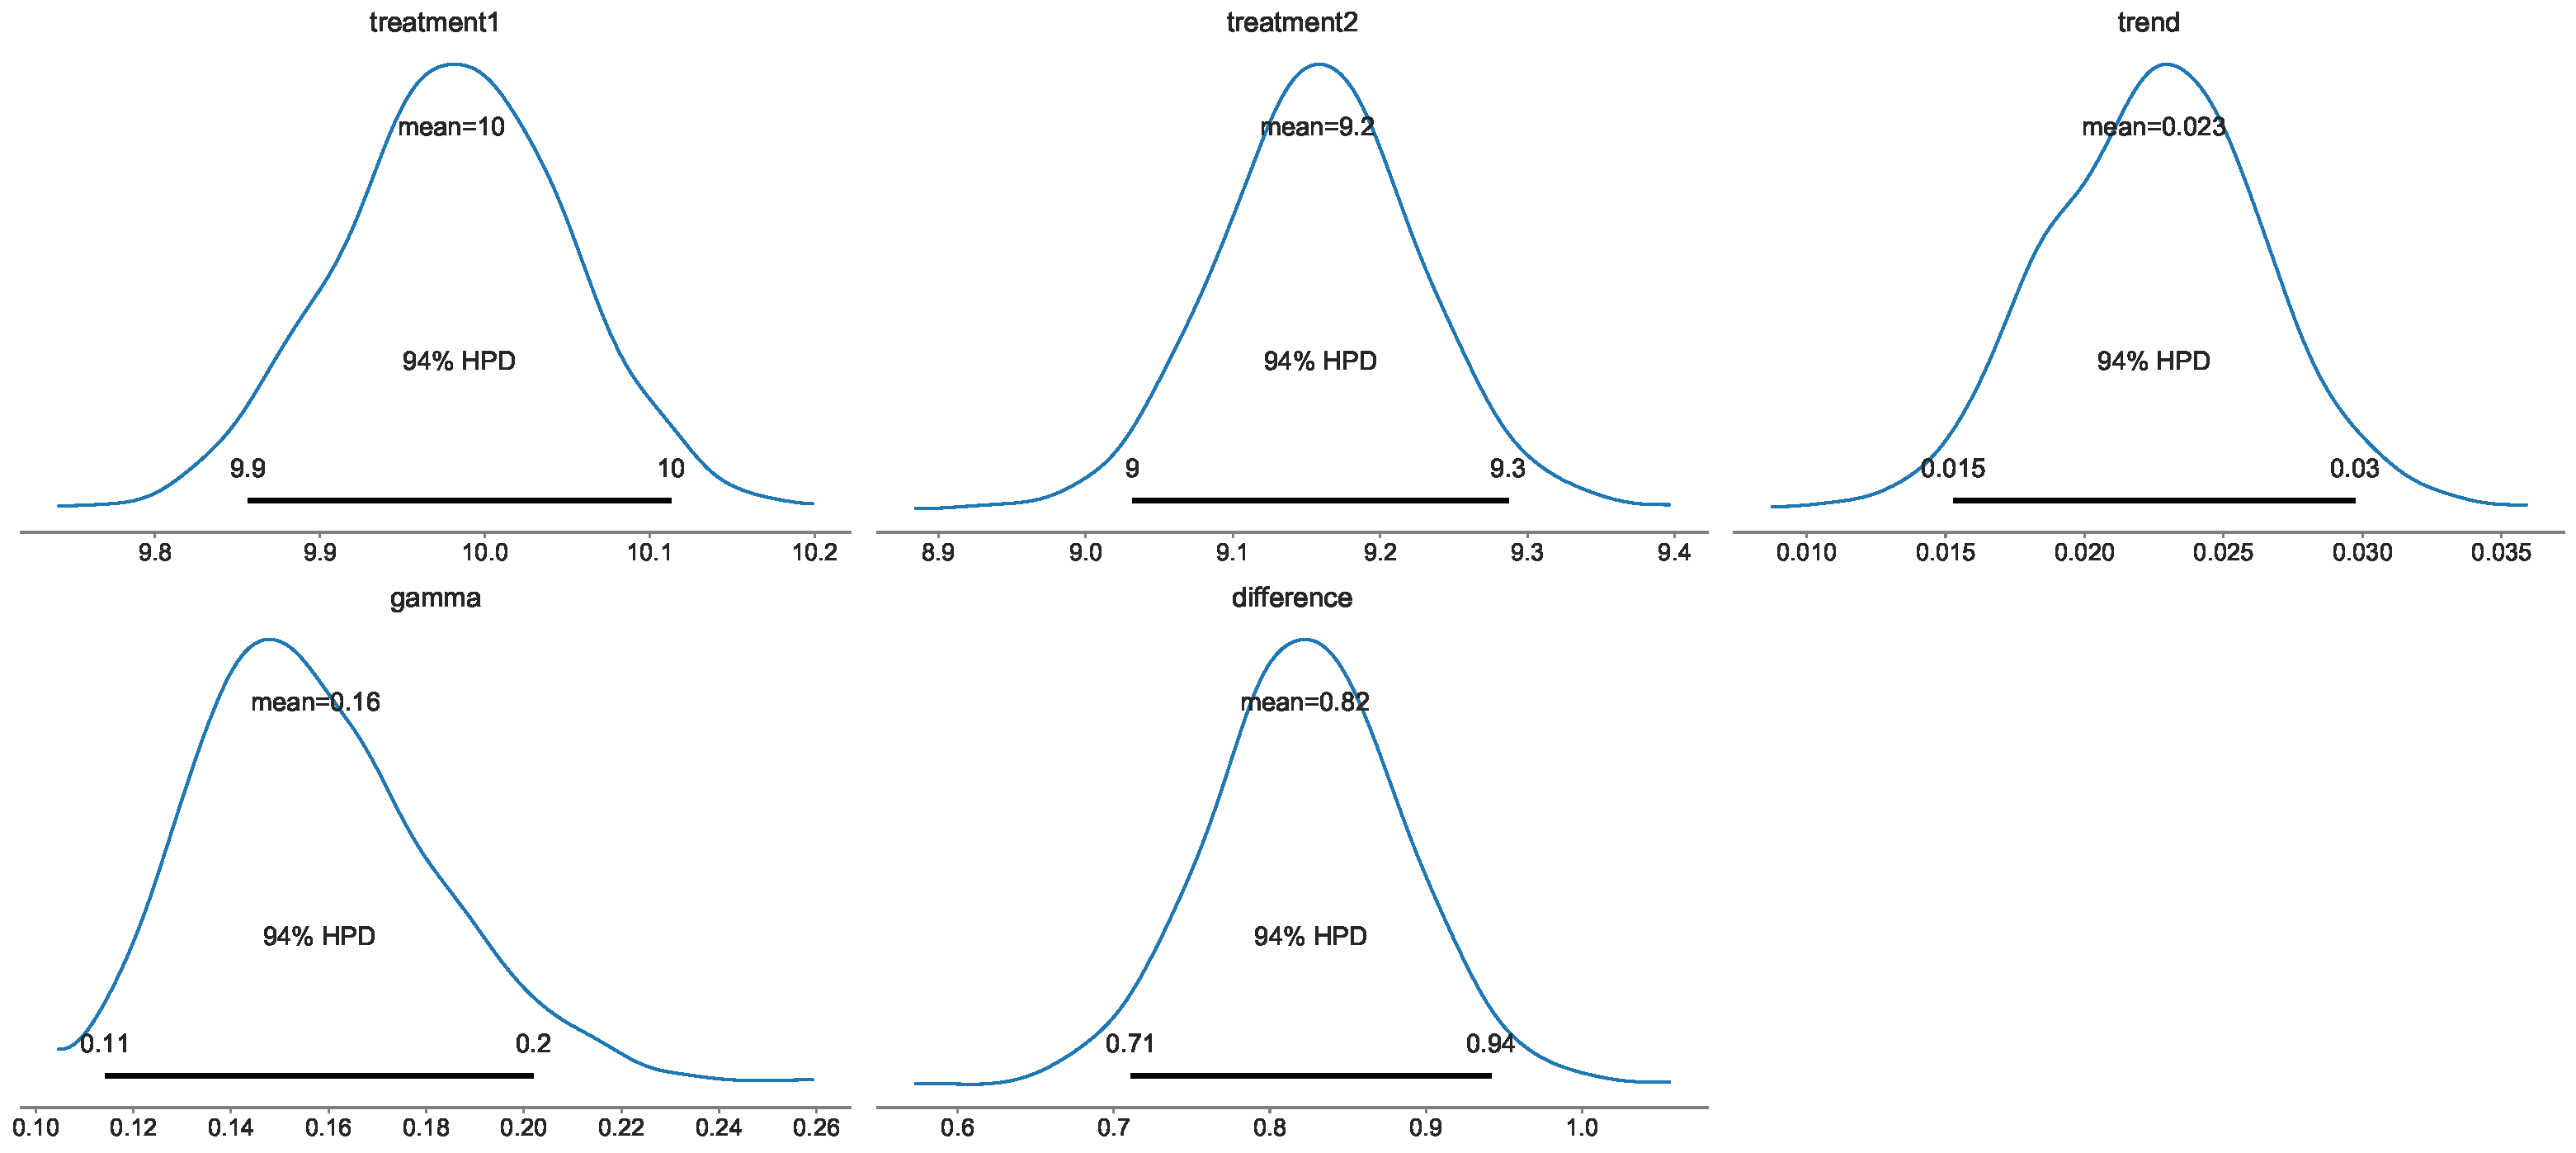
\includegraphics[width=\textwidth,height=\textheight,keepaspectratio]{single_patient_posteriors.pdf}
\end{figure}
\bigskip

The inbuilt PyMC3 method prints the posterior distribution for all of our parameters,
with their posterior mean and highest posterior density interval (HPD) for approximately
95 \% of the values\footnote{The default HPD in PyMC3 plots is 94 \% just to underline that the common
95 \% standard is arbitrary.}. We can see that even though the posterior means between
the two treatment options are clearly different, there is some overlap. When
trying to estimate the difference of the parameters we should not trust the posteriors of
the individual parameters, as this does not take into account the possible depencies
between these. For this reason, we defined the difference between these two
parameters as a separate deterministic parameter and can now use it to give us the result we are interested in. We can see
that for this difference the mean is positive and the HPD does not include zero, so we can be quite certain that
treatment A is a worse option for this patient than treatment B, with the likely values of
the difference falling roughly between 0.3 and 0.8.

\subsubsection*{Part 9: Checking Model Fit with Posterior Sampling}

\bigskip
\begin{pyverbatim}[][fontsize=\footnotesize]
    with single_patient_no_trend_model as model:
        post_pred = pm.sample_posterior_predictive(trace, samples=500)
        predictions = post_pred["y"]

    draw_posterior_checks(
        predictions=predictions,
        measurements_df=measurements_df[patient_idx == 0],
        parameters_df=parameters_df[parameters_df["patient_idx"] == 0],
        plot_name="single_patient_posterior_sampling",
    )
\end{pyverbatim}
\smallskip

There is still one important thing that we should check before announcing our results: we should
make sure that our model is a good fit for our data. Even if we have precise
results, if our model does a poor job at reflecting the reality, we should not get too
excited.
Checking model fit for Bayesian models can be done with posterior sampling. We start by generating samples from
the posterior distributions and for each of these samples, we create a simulated dataset based
on the chosen parameter values that replicate the experiment. Then we compare these
simulated datasets to the actual data. What we want to see is that actual data looks
like a typical simulated dataset.

The logic behind this can be appreciated by thinking of a comparison between a case
where the real data is created with a mean and a strong trend, but our model only includes a
mean. Even if our parameter estimates are very precise, the data simulated based on our
model can never match the shape of the real data. On the other hand, if we include the trend in our
model now the model replicates perfectly the data creation process and
the only difference with the real data and simulated data is that the real data was
created by the real parameter values, whereas the simulated data was created with
estimated values for these parameters. In this case, the values of the simulated data
should spread around the real values with random errors determined by the degree
of uncertainty we have on the posterior values. In the real world creating a model that
matches the data creation process exactly is rare outside laboratory experiments, but
the principle still holds: a good model should be a good description of the reality and
the data created based on its estimates should be hard to distinguish from the real
data, with little or no systematic errors\footnote{Of course this might not be true if the
real data is a true outlier.}.

PyMC3 has an inbuilt method for taking the posterior samples. This function needs access
to the original model so we use it in the context manager
to give it access to this. With the simulated samples, we can recreate a timeline of
measurements and see how well the simulated timelines match with the real data.
This can be seen in figure\ \ref{singlepatientposteriortimeline}.
All 500 samples are drawn as grey lines with one sample highlighted with a blue line and
the actual measurement with a red line. We can see that the results line up quite
nicely with sampled values spread around the values of the real measurements.

\bigskip
\begin{figure}[H]
    \caption{Single Patient Posterior Sample Timeline}\label{singlepatientposteriortimeline}
    \bigskip
    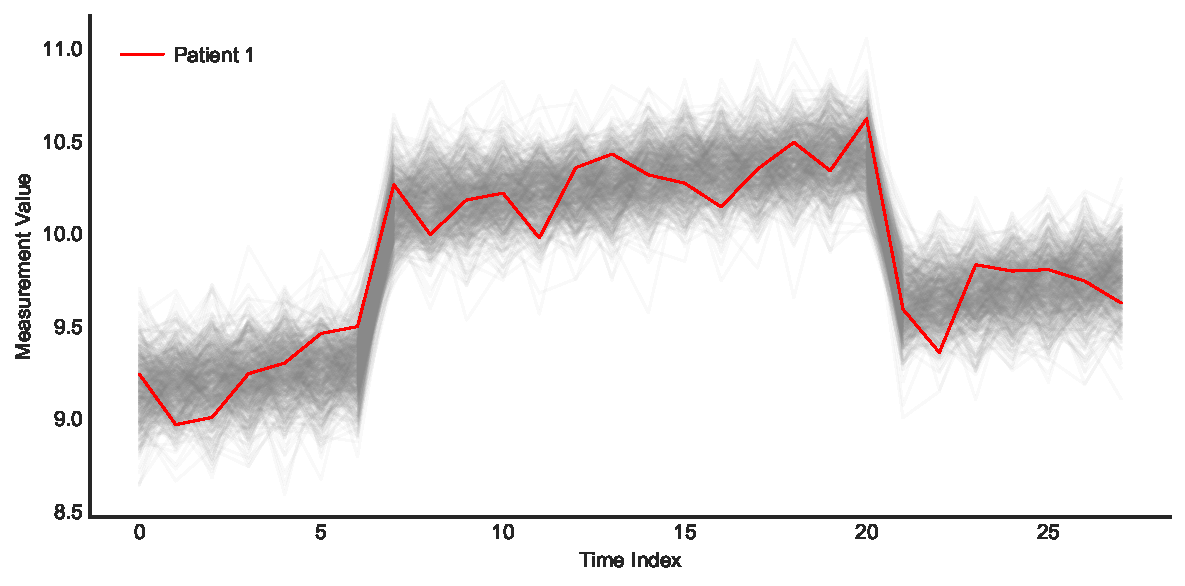
\includegraphics[width=\textwidth,height=\textheight,keepaspectratio]{posterior_sample_timeline_single_patient.pdf}
\end{figure}
\bigskip

For more precise comparison we have written a special function
\pyv{draw_posteriors()}. We don't go over the code of this function,
but what it does is to use the datasets created by the PyMC3 inbuilt method and
calculates from each posterior sample the mean of the measurements under each treatment and the difference between
these means. It then plots the distribution of these values
against the values calculated from the
original data. For the difference between the means, it also plots the actual
difference of the true parameters making it possible to see how accurate the model really
is. The graphs created by this function can be seen in figure\
\ref{singlepatientposteriorsampling}.
We see that the distribution of the mean treatment effectiveness calculated from the
posterior samples matches nicely with the actual mean of the data. There is also a good
match when comparing the true difference in the parameter values with the distribution of
the difference in the simulated datasets. This indicated that our
model seems to be a good approximation of reality.

\bigskip
\begin{figure}[H]
    \caption{Single Patient Posterior Sampling}\label{singlepatientposteriorsampling}
    \bigskip
    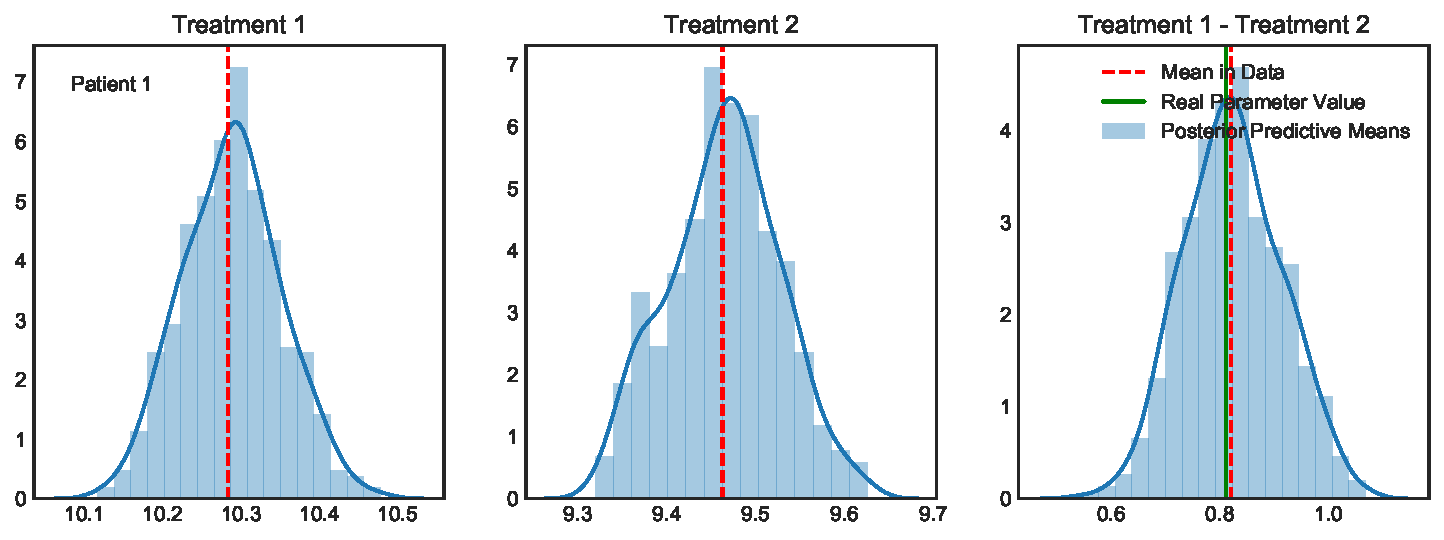
\includegraphics[width=\textwidth,height=\textheight,keepaspectratio]{single_patient_posterior_sampling.pdf}
\end{figure}
\bigskip

\subsection{Results and Interpretation}

We have now completed the single patient analysis after going through the following steps:

\begin{enumerate}
    \item Define the model and the priors
    \item Implement the model in PyMC3
    \item Calculate the results
    \item Evaluate the estimation process
    \item Check the posterior values
    \item Make sure that the model is an accurate enough description of reality
\end{enumerate}

In real-world analysis, we would also add step 0: cleaning and exploring the data.
Based on our results, we can say that for patient 1 treatment B is recommended over treatment A
with the most probable difference in treatment effect effectiveness being 0.55
measurement points in favour of treatment B. We can also easily communicate
the uncertainty in our estimation with the HPD by saying that the true difference of
the treatments is with 95 \% probability between 0.3 and 0.8. As we have the full
posterior difference distribution, we can also visually show these results with a graph,
which is the clinical setting probably the most advisable solution. The important thing
to underline here is that we are talking about actual probabilities and not likelihoods,
circumventing complicate definitions and having intuitively understandable results.

\section{Analyzing Multiple Trials With Hierarchical Models}\label{pooling}

Repeating the single patient model for all patients is a completely viable strategy for
getting estimates for all patients, but we can do better by making the model
hierarchical and utilizing intelligent pooling of patient data. To do this we need to
modify our model to include population-level distribution and define the priors for this
level. The new parameters add complexity to the model and we need to make some changes
in how we implement the model to ensure efficient sampling.

\subsection{Defining the Model}\label{hiermodel}

We start with the same model that we used for the single patient, but now we index all our
measurements not just by time \(t\), but also by patient \(j\):

\begin{def}\label{hierarchicalmodel}
    \begin{equation}\label{}
        y_{tj} = Z_{tj}\theta_{j} + W_{tj}\eta_{j} + t\beta_{j} + \epsilon_{tj}
    \end{equation}
\end{def} where \(\theta_{j} \) and \(\eta_{j} \) are the patient-specific treatment
effects with \(Z_{tj}\) and \(W_{tj}\) being indicator
variables that are 1 when observation \(t\) is within a period where treatment was applied and
0 otherwise. These are also patient-specific as the order of treatments was randomly
chosen for each patient. \(\beta_j\) is the trend representing the natural progress of the
condition. \(\epsilon_{tj} \sim N(0,\tau_j^2) \) is the error term at \(t\) and
\(\rho_j\) is the correlation between consecutive errors.

To make this model hierarchical we now add the population-level distributions which
the patient-level parameters are drawn from and the priors for this parameter layer.
We add hierarchy for all the parameters except the patient-level measurement error, as
we are not that interested in the population-level of this parameter and adding it
would make the model unnecessarily complex.

\bigskip
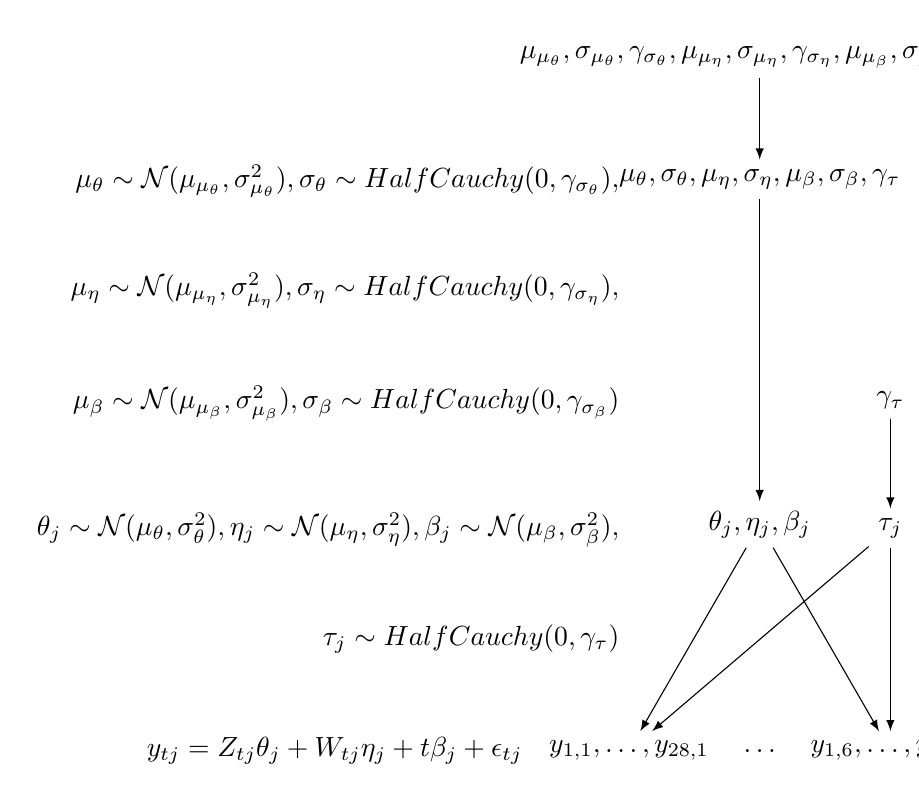
\begin{tikzpicture}

    \matrix[matrix of math nodes, column sep=-75pt, row sep=30pt] (mat)
    {
        \ & \mu_{\mu_{\theta}}, \sigma_{\mu_{\theta}},
        \gamma_{\sigma_{\theta}},
        \mu_{\mu_{\eta}}, \sigma_{\mu_{\eta}},
        \gamma_{\sigma_{\eta}},
        \mu_{\mu_{\beta}}, \sigma_{\mu_{\beta}},
        \gamma_{\sigma_{\beta}} \\
        \ & \mu_{\theta}, \sigma_{\theta}, \mu_{\eta},\sigma_{\eta}, \mu_{\beta}, \sigma_{\beta}, \gamma_{\tau} & \ \\
        \ \\
        \ & \ & \gamma_{\tau} \\
        \ & \theta_j, \eta_j, \beta_j & \tau_j & \\\
        \ \\
        y_{1,1}, \ldots, y_{28, 1} & \ldots & y_{1,6}, \ldots, y_{28, 6} \\
    };

    \draw[->,>=latex] (mat-1-2) -- (mat-2-2);
    \draw[->,>=latex] (mat-2-2) -- (mat-5-2);
    \draw[->,>=latex] (mat-4-3) -- (mat-5-3);
    \draw[->,>=latex] (mat-5-2) -- (mat-7-1);
    \draw[->,>=latex] (mat-5-2) -- (mat-7-3);
    \draw[->,>=latex] (mat-5-3) -- (mat-7-1);
    \draw[->,>=latex] (mat-5-3) -- (mat-7-3);

    \node[anchor=east] at ([xshift = 0pt]mat-2-1)
    {$
        \mu_{\theta} \sim \mathcal{N}(\mu_{\mu_{\theta}}, \sigma^2_{\mu_{\theta}}),
        \sigma_{\theta} \sim HalfCauchy(0, \gamma_{\sigma_{\theta}}),
    $};
    \node[anchor=east] at ([xshift = 0pt]mat-3-1)
    {$
        \mu_{\eta} \sim \mathcal{N}(\mu_{\mu_{\eta}}, \sigma^2_{\mu_{\eta}}),
        \sigma_{\eta} \sim HalfCauchy(0, \gamma_{\sigma_{\eta}}),
    $};
    \node[anchor=east] at ([xshift = 0pt]mat-4-1)
    {$
        \mu_{\beta} \sim \mathcal{N}(\mu_{\mu_{\beta}}, \sigma^2_{\mu_{\beta}}),
        \sigma_{\beta} \sim HalfCauchy(0, \gamma_{\sigma_{\beta}})
    $};
    \node[anchor=east] at ([xshift = 0pt]mat-5-1)
    {$
        \theta_{j} \sim \mathcal{N}(\mu_{\theta},\sigma_{\theta}^2),
        \eta_{j} \sim \mathcal{N}(\mu_{\eta},\sigma_{\eta}^2),
        \beta_{j} \sim \mathcal{N}(\mu_{\beta},\sigma_{\beta}^2),
    $};
    \node[anchor=east] at ([xshift = 0pt]mat-6-1)
    {$
        \tau_{j} \sim HalfCauchy(0, \gamma_{\tau})
    $};
    \node[anchor=east] at ([xshift = -35pt]mat-7-1)
    {$
        y_{tj} = Z_{tj}\theta_{j} + W_{tj}\eta_{j} + t\beta_{j} + \epsilon_{tj}
    $};
\end{tikzpicture}

As the priors are defined on the population-level, we have to think a bit differently when defining the
parameters of these distributions as we are now talking about a different level of
analysis. For prior values for the means of the treatment effect and trend means
we can obviously use the same means as in single patient model (10 for both treatments and 0.2 for
trend), but standard deviation needs some consideration. As in this case we are talking about the
distribution of means we should use the estimated standard error instead of standard
deviation from the existing patient data. With the estimate of the standard error of the mean being defined as
\( \sigma_{y} \approx \frac{s}{\sqrt{n}} \), we can just divide the standard deviations
we calculated for the single patient model with 5 (\(\sqrt{25} = 5\)) and end up with
prior values for the standard deviation of the treatment effect means being 0.6 and 0.16 for the trend. Remember that
we already multiplied the actual calculated standard deviations by 2 in the single
patient model, so we are still adjusting for the uncertain representativeness of the
existing data. The case for the priors of standard deviations for treatment effects and
trends is interesting. Here can just use the standard deviations we calculated for
the single patient model for the scale values. What this means in practice is that we expect the
median of the real standard deviations to be this number, but as we are using
half-Cauchy that has a long tail, this is only a minimal, but still informed,
constraint. With treatment errors being not hierarchical we will use the same prior value
of 1 for the scale as we did in the single patient model. The chosen priors values for
our hierarchical model are summarized in table\ \ref{hierarchicalmodelpriorvalues}.

\begin{table}[H]
    \caption{Hierarchical Model Prior Values}\label{hierarchicalmodelpriorvalues}
    \begin{align}\label{}
        \text{population treatment A mean mean prior: } & \mu_{\mu_{\theta}} = 10 \nonumber \\
        \text{population treatment A mean standard deviance prior: } & \sigma_{\mu_{\theta}} = 0.6 \nonumber \\
        \text{population treatment A standard deviance prior: } & \gamma_{\sigma_{\theta}} = 3 \nonumber \\
        \text{population treatment B mean mean prior: } & \mu_{\mu_{\eta}} = 10 \nonumber \\
        \text{population treatment B mean standard deviance prior: } & \sigma_{\mu_{\eta}} = 0.6 \nonumber \\
        \text{population treatment B standard deviance prior: } & \gamma_{\sigma_{\eta}} = 3 \nonumber \\
        \text{population trend mean mean prior: } & \mu_{\mu_{\beta}} = 0.2 \nonumber \\
        \text{population trend mean standard deviance prior: } & \sigma_{\mu_{\beta}} = 0.16 \nonumber \\
        \text{population trend standard deviance prior: } & \gamma_{\sigma_{\beta}} = 0.8 \nonumber \\
        \text{measurement error scale prior: } & \gamma_{\tau} = 1 \nonumber
    \end{align}
\end{table}

\subsection{Implementing the Model in PyMC3}

Next, we move to implement our hierarchical model in PyMC3. As by now we are already
familiar with the basics of PyMC3, we can skip explaining most of the code to focus
just on the differences with the single patient model. The reader will quickly
see that the model we have here is quite different and we will give the reasons behind this a lot of focus. Here is the full
implementation, that we will afterwards break down piece by piece:

\bigskip
\begin{pyverbatim}[][fontsize=\footnotesize]
with pm.Model() as hierarchical_with_trend_model:

    # population priors
    pop_treatment_a_mean = pm.Normal("Population Treatment A Mean", mu=10, sigma=0.6)
    pop_treatment_a_sd = pm.HalfCauchy("Population Treatment A Sd", beta=3)
    pop_treatment_b_mean = pm.Normal("Population Treatment B Mean", mu=10, sigma=0.6)
    pop_treatment_b_sd = pm.HalfCauchy("Population Treatment B Sd", beta=3)
    pop_trend_mean = pm.Normal("Population Trend Mean", mu=0.2, sigma=0.16)
    pop_trend_sd = pm.HalfCauchy("Population Trend SD", beta=0.8)

    # modelling patient difference from population with offset parameters
    pat_treatment_a_offset = pm.Normal(
        "Treatment A Offset", mu=0, sigma=1, shape=patients_n
    )
    pat_treatment_b_offset = pm.Normal(
        "Treatment B Offset", mu=0, sigma=1, shape=patients_n
    )
    pat_trend_offset = pm.Normal("Trend Offset", mu=0, sigma=1, shape=patients_n)

    # separate deterministic parameter for each patient
    pat_treatment_a = pm.Deterministic(
        "Treatment A",
        pop_treatment_a_mean + pat_treatment_a_offset * pop_treatment_a_sd,
    )
    pat_treatment_b = pm.Deterministic(
        "Treatment B",
        pop_treatment_b_mean + pat_treatment_b_offset * pop_treatment_b_sd,
    )
    pat_trend = pm.Deterministic(
        "Trend", pop_trend_mean + pat_trend_offset * pop_trend_sd
    )

    # variance is not hierarchical
    pat_gamma = pm.HalfCauchy("Gamma", beta=1, shape=patients_n,)

    # creating a vector defining the expected means of the observations
    # which are defined by one of the treatment means + trend
    measurement_means = (
        pat_treatment_a[patient_idx] * measurements_df["treatment_a"]
        + pat_treatment_b[patient_idx] * measurements_df["treatment_b"]
        + pat_trend[patient_idx] * measurements_df["measurement"]
    )

    # likelihood is multivariate normal distribution with the same amount of dimensions
    # as the patients has measurements with means defined by the previously
    # defined vector and the variance vector
    likelihood = pm.Normal(
        "y",
        measurement_means,
        sigma=pat_gamma[patient_idx],
        observed=measurements_df["measurement"],
    )

    # adding the comparison between the treatments
    pop_difference = pm.Deterministic(
        "Population Treatment Difference (A-B)",
        pop_treatment_a_mean - pop_treatment_b_mean,
    )
    pat_difference = pm.Deterministic(
        "Treatment Difference (A-B)", pat_treatment_a - pat_treatment_b
    )

    # running the model
    trace = pm.sample(draws=5000, tune=3000, cores=3, target_acceptance=0.95)

    # Checking diagnostic describing how the algorithm performed
    pm.traceplot(
        trace,
        var_names=[
            "Population Treatment A Mean",
            "Population Treatment A Sd",
            "Population Treatment B Mean",
            "Population Treatment B Sd",
            "Population Trend Mean",
            "Population Trend SD",
        ],
    )
    plt.show()
    pm.traceplot(
        trace,
        var_names=["Treatment A", "Treatment B", "Trend", "Gamma"],
    )
    plt.show()
    pm.summary(hierarchical_trace, kind="diagnostics")

    # checking the posterior distributions
    pm.plot_posterior(
        trace,
        var_names=[
            "Population Treatment A Mean",
            "Population Treatment B Mean",
            "Population Treatment Difference (A-B)",
            "Population Trend Mean",
        ],
        credible_interval=0.95,
    )
    plt.show()
    pm.plot_posterior(
        trace,
        var_names=["Treatment Difference (A-B)"],
        credible_interval=0.95,
    )
    plt.show()

# creating new observations based on our model with sampled
with hierarchical_with_trend_model as model:
    post_pred = pm.sample_posterior_predictive(
        trace, samples=500
    )
    predictions = hierarchical_post_pred["y"]

# visualizing posterior samples to check the model's match with reality
draw_posterior_checks(
    predictions=predictions,
    measurements_df=measurements_df,
    parameters_df=parameters_df,
)
\end{pyverbatim}
\bigskip

\subsubsection*{Part 1: Defining the population-level Priors}

\bigskip
\begin{pyverbatim}[][fontsize=\footnotesize]
    pop_treatment_a_mean = pm.Normal("Population Treatment A Mean", mu=10, sigma=0.6)
    pop_treatment_a_sd = pm.HalfCauchy("Population Treatment A Sd", beta=3)
    pop_treatment_b_mean = pm.Normal("Population Treatment B Mean", mu=10, sigma=0.6)
    pop_treatment_b_sd = pm.HalfCauchy("Population Treatment B Sd", beta=3)
    pop_trend_mean = pm.Normal("Population Trend Mean", mu=0.2, sigma=0.16)
    pop_trend_sd = pm.HalfCauchy("Population Trend SD", beta=0.8)
\end{pyverbatim}
\bigskip

With the population-level priors we use the exact same method that we used when we were
defining priors in the single patient model. All the distributions that we use are
inbuilt in PyMC3, so no complex procedures are needed here.

\subsubsection*{Part 2: Defining the patient-level Parameters}

\bigskip
\begin{pyverbatim}[][fontsize=\footnotesize]
    pat_treatment_a_offset = pm.Normal(
        "Treatment A Offset", mu=0, sigma=1, shape=patients_n
    )
    pat_treatment_b_offset = pm.Normal(
        "Treatment B Offset", mu=0, sigma=1, shape=patients_n
    )
    pat_trend_offset = pm.Normal("Trend Offset", mu=0, sigma=1, shape=patients_n)

    pat_treatment_a = pm.Deterministic(
        "Treatment A",
        pop_treatment_a_mean + pat_treatment_a_offset * pop_treatment_a_sd,
    )
    pat_treatment_b = pm.Deterministic(
        "Treatment B",
        pop_treatment_b_mean + pat_treatment_b_offset * pop_treatment_b_sd,
    )
    pat_trend = pm.Deterministic(
        "Trend", pop_trend_mean + pat_trend_offset * pop_trend_sd
    )
    pat_gamma = pm.HalfCauchy("Gamma", beta=1, shape=patients_n,)
\end{pyverbatim}
\smallskip

When defining the patient level parameters we see something quite different from the
single patient model that is also seemingly at odds with our model definition. Instead
of modelling the patient parameters as coming from the population distributions, we model
them as being that same value as the population distribution with an offset scaled by
the population level standard deviations. Although this looks like we made some radical
change to our previously defined model, in practice the model is still the same and
the changes are just made to ensure efficient sampling.

The problem with hierarchical
models where standard deviation parameters are hierarchical is that when the sampler is
exploring the part of posterior distribution where the higher-level standard deviation values
are close to zero the sampler can easily get stuck. This happens because
when the population standard deviation is close to zero the patient level parameters
have very tiny parameter space where the values are reasonable as they have match almost
perfectly with the population level values. This, in turn, will mean
that most of the values suggested by the sampler in this space are highly improbable and
most of the steps will not be accepted leaving the chain stuck in place and leading to
unrepresentative samples. We can fix this by breaking the strong dependency of the
parameters being estimated with using offsets. With this method, when the value of the
population-level standard deviations are close to zero, the offset (unlike the
patient-level parameter value) is not constrained to tight parameter space as because it is
multiplied by the population-standard deviation and thus almost any value given to it is
plausible as now it has minimal impact on the actual patient-level treatment effect.
Now there is much less chance for the chains to get stuck and sampling is more
efficient. Importantly this way of parameterizing the model has minimal impact on the end
results and we don't have to worry it much when interpreting the results. It is
important to note that patient-level parameters are implemented with PyMC3
\pyv{deterministic}-function as these are now completely deterministic when conditioned
on the parameter values that constitute it.\cite{offset}

With the fact that we have multiple patients, but these share the same parameters,
we can implement this easily in PyMC3, by defining the dimensions of the distribution
with the \pyv{shape} argument that is given an argument containing an integer that tells
the number of patients that we have. This argument can be seen used in the offsets, but not in the
deterministic patient-level parameters as the multidimensional offset used in these
makes them multidimensional automatically.

\subsubsection*{Part 3: Defining the Likelihood}

\bigskip
\begin{pyverbatim}[][fontsize=\footnotesize]
    measurement_means = (
        pat_treatment_a[patient_idx] * measurements_df["treatment_a"]
        + pat_treatment_b[patient_idx] * measurements_df["treatment_b"]
        + pat_trend[patient_idx] * measurements_df["measurement"]
    )

    likelihood = pm.Normal(
        "y",
        measurement_means,
        sigma=pat_gamma[patient_idx],
        observed=measurements_df["value"],
    )
\end{pyverbatim}
\smallskip

Defining the likelihood is done in the same way as we did with the single patient model,
with imaging the data as one sample from a multidimensional distribution with as many
dimensions as there are observations. In this case, the
distribution will have 168 dimensions (28 measurements X 6 patients = 168). We
create the means of this distribution by turning the treatment and trend means from
a vector of length 6 (one value for each patient) to a vector of length 168 with the
\pyv{patient_idx} vector. This vector has a length 168 and its values are the indices of the
patients with the first 28 values being
zero representing the measurements of patient 1, next 28 values being 1 representing
patient 2 and so on. By indexing the treatment mean and trend vectors with this vector the end
product is a vector of length 168, with each patient being represented 28 times
in a row. We then combine these vectors to a single treatment mean vector by multiplying
the treatment mean parts with the treatment indicators and the trend with the
measurement index (0--27) and then sum these together. The end result is a
vector of length 128 with each patient being represented with 28 sequential values that
combine the mean of the treatment taken at that time point and the trend times measurement index. The standard
deviation of the distribution is also turned into a vector of length 168 with the
\pyv{patient_idx} vector. Note that unlike in the single patient case, where we could use a single
standard deviation value even though we had multiple means, in this case, we have to
provide a vector with a length that matches the length of the vector of the means as we
want to use different standard deviations for different patients.

\subsubsection*{Part 4: Running the Model}

\bigskip
\begin{pyverbatim}[][fontsize=\footnotesize]
    trace = pm.sample(draws=5000, tune=3000, cores=3, target_acceptance=0.95)
\end{pyverbatim}
\bigskip

As our model is now much more complex than with the single patient model with much
more parameters, we need to use more tuning and calculation steps. We have to bump the tuning steps from 600 to all the way to
3000 and the calculation steps from 1000 to 3000. As we will see even this does not
avoid all problems, but gives us a big enough effective sample size and ensures that
chains will converge. To prevent the chains from getting stuck we also increase the target
step acceptance probability \pyv{target_acceptance} from the default 80 \% to 95 \%.
This forces the NUTS-sampler to take smaller steps, that makes the sampling less
efficient, but will make it less likely that the chains will end up in a situation where
they cannot move at all. With the high number of steps we are taking, the reduced
efficiency should not be a problem. Just like in the single patient model we still use 3
chains and now all these chains will take steps in the multidimensional posterior defined not
just by patient parameters, but also the population parameters (in practice the offsets).

\subsubsection*{Part 5: Checking Algorithm Diagnostics}

\bigskip
\begin{pyverbatim}[][fontsize=\footnotesize]
    pm.traceplot(
        trace,
        var_names=[
            "Population Treatment A Mean",
            "Population Treatment A Sd",
            "Population Treatment B Mean",
            "Population Treatment B Sd",
            "Population Trend Mean",
            "Population Trend SD",
        ],
    )
    plt.show()
    pm.traceplot(
        trace,
        var_names=["Treatment A", "Treatment B", "Trend", "Gamma"],
    )
    plt.show()
    pm.summary(hierarchical_trace, kind="diagnostics")
\end{pyverbatim}
\bigskip

When checking algorithm diagnostic the amount of parameters is now so big that it makes
sense to separate the traceplots into multiple chunks. We start with the population
traceplots as these look similar to the traceplots in the single patient
model. In figure\ \ref{hierarchicalmodelpopulationtraceplots} we can see traceplots for each of
the 6 population-level parameters. Once again, we hope to see that the time series looks
like noise and that the posterior distributions of the chains align nicely. Everything
seems to be in order except that we have these black dashes at the bottom of the graphs.
These mark the divergences of the chains. These mark parts where the chain finds itself
stuck in one part of the distribution for unexpectedly long. If we did not
parametrize our model with the offsets, we would have much more of these.

\bigskip
\begin{figure}[H]
    \caption{Hierarchical Model population-level Traceplots}\label{hierarchicalmodelpopulationtraceplots}
    \bigskip
    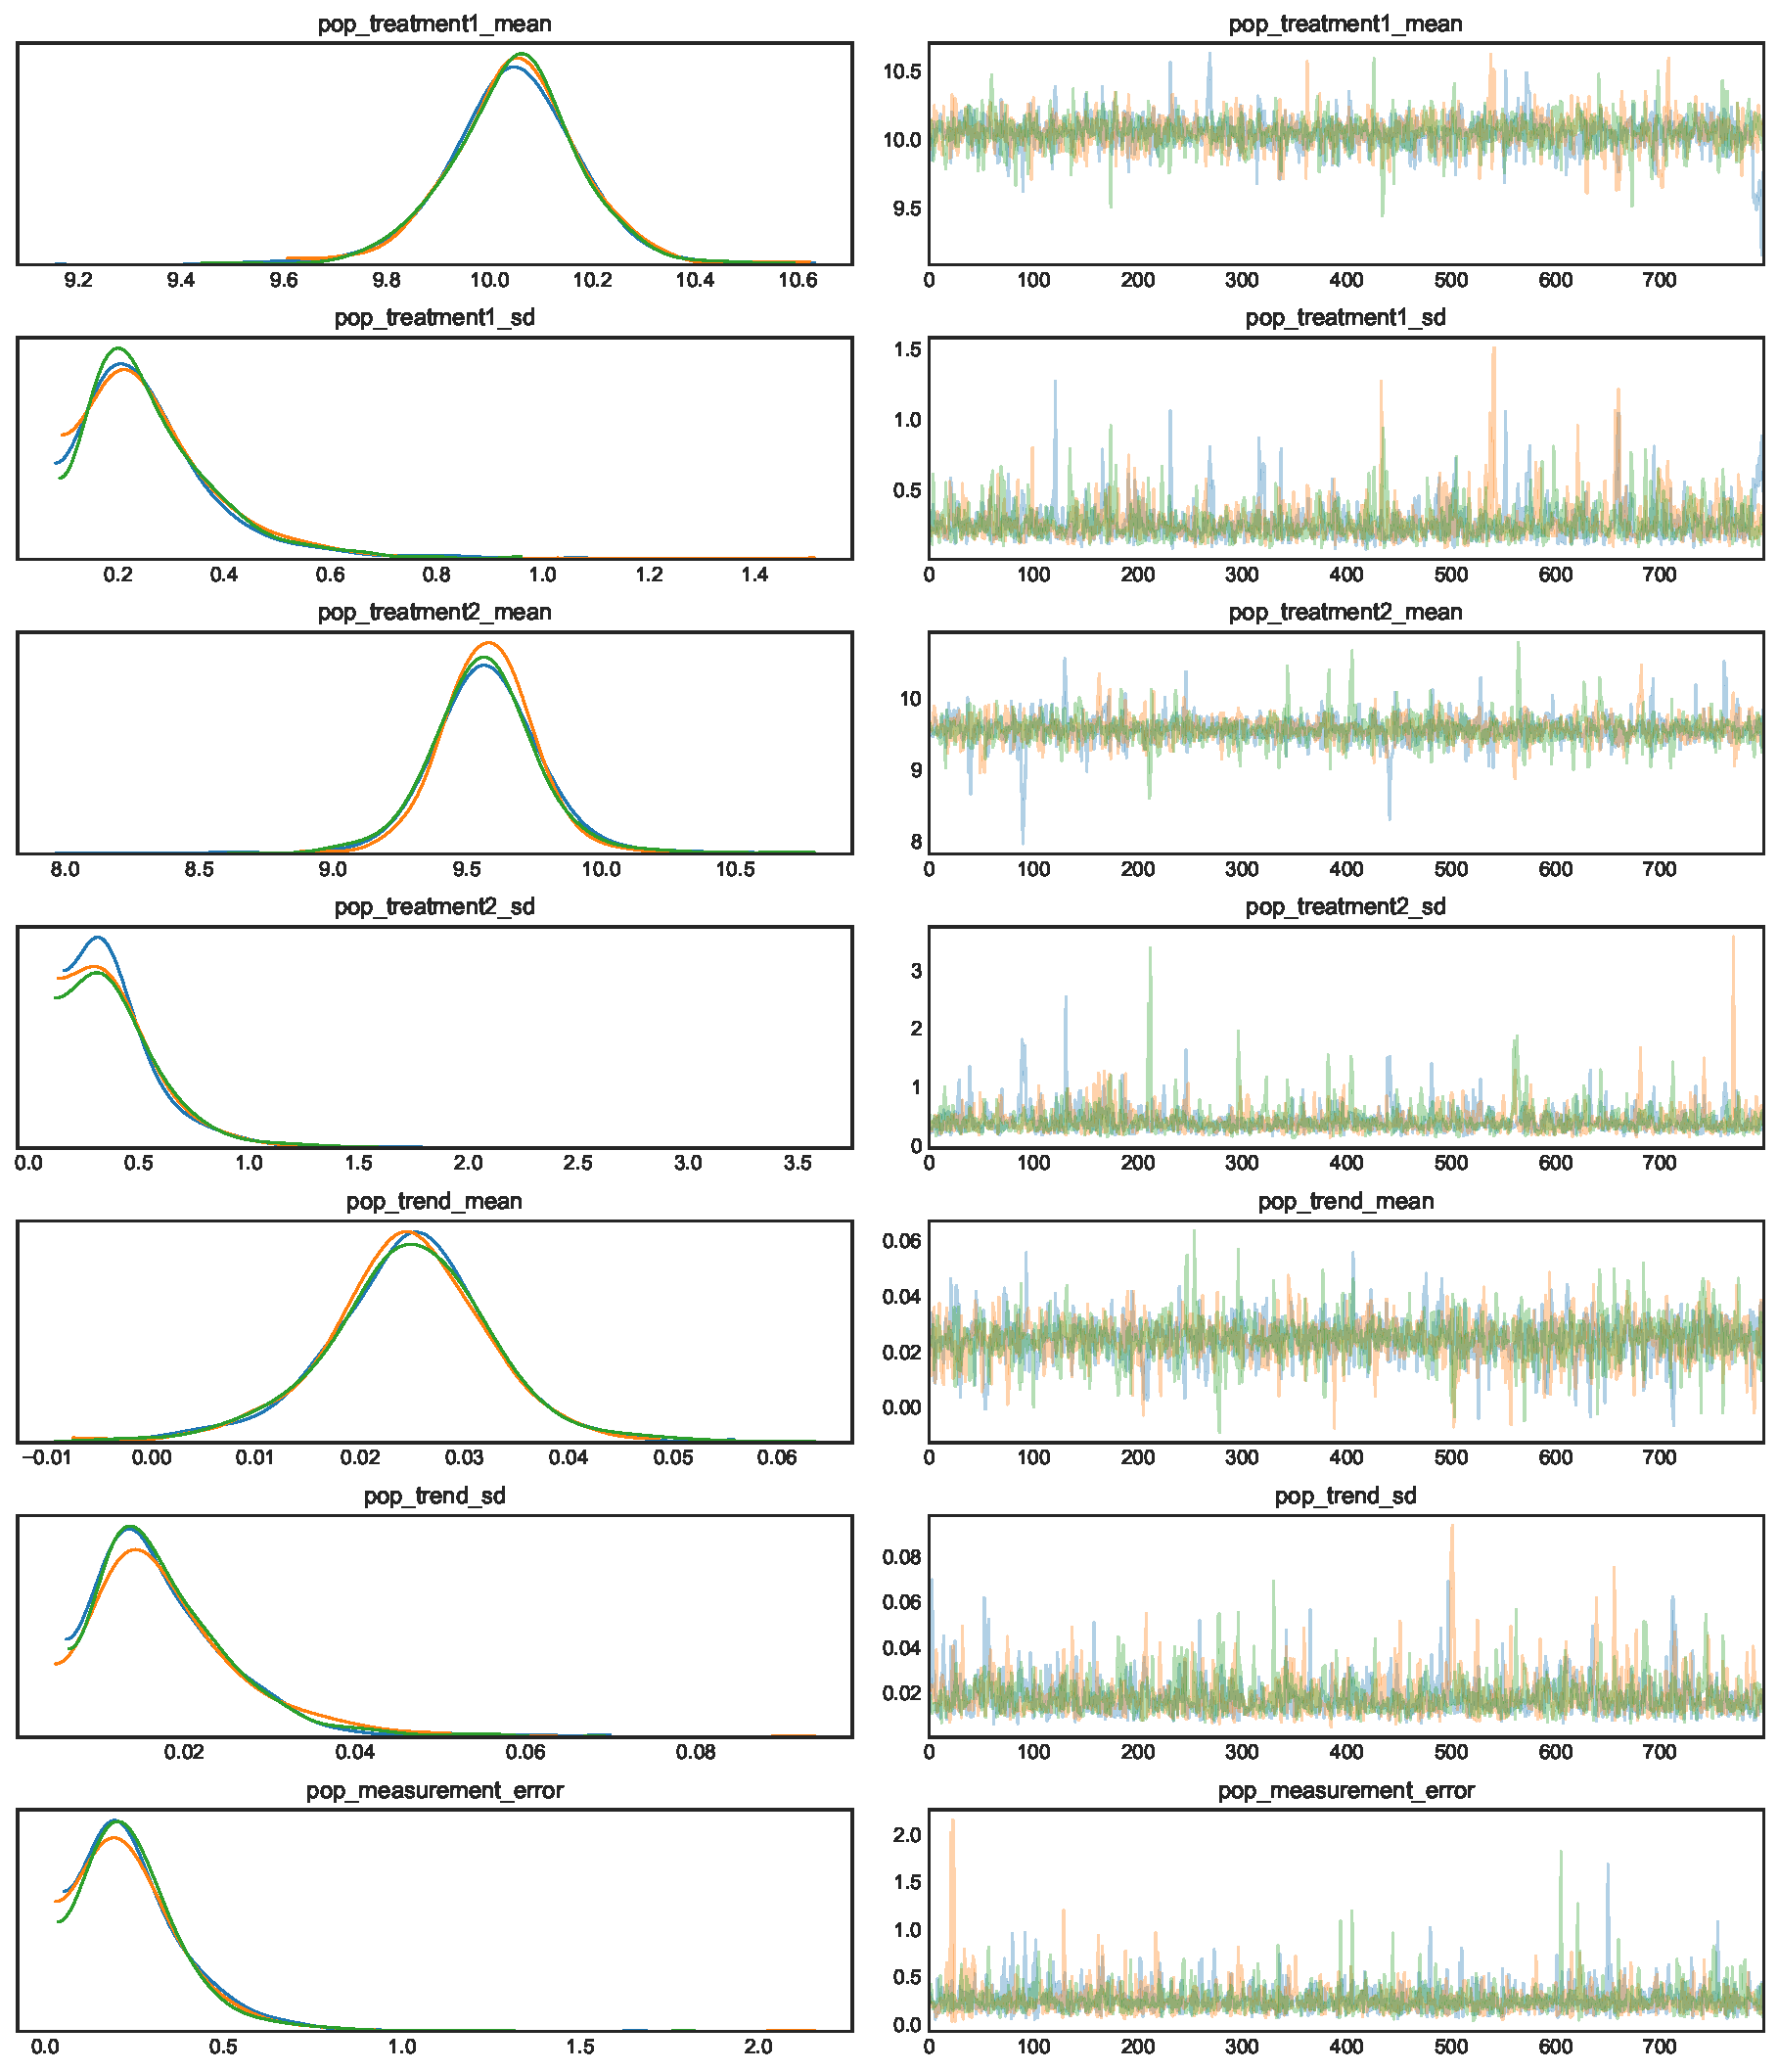
\includegraphics[width=\textwidth,height=\textheight,keepaspectratio]{hierarchical_model_population_level_traceplot.pdf}
\end{figure}
\bigskip

Next, we check the traceplots of the patient-level parameters in
figure\ \ref{hierarchicalmodelpatienttraceplots}. These look a bit different now as the patient
level parameters are multidimensional with every patient having their own
parameter. This makes the right side of the plot hard to interpret, but the left side is
still intelligible and we see that the posteriors of the three chain align even though
we have lots of divergences. It is possible to plot the traceplots for single patients
by passing the indices of parameters to be plotted in a Python dictionary to ``coords''
parameter in the traceplot function. This is more work but is worth it if the
left side of the plot seems problematic. In this case everything looks okay, so we skip this.

\bigskip
\begin{figure}[H]
    \caption{Hierarchical Model patient-level Traceplots}\label{hierarchicalmodelpatienttraceplots}
    \bigskip
    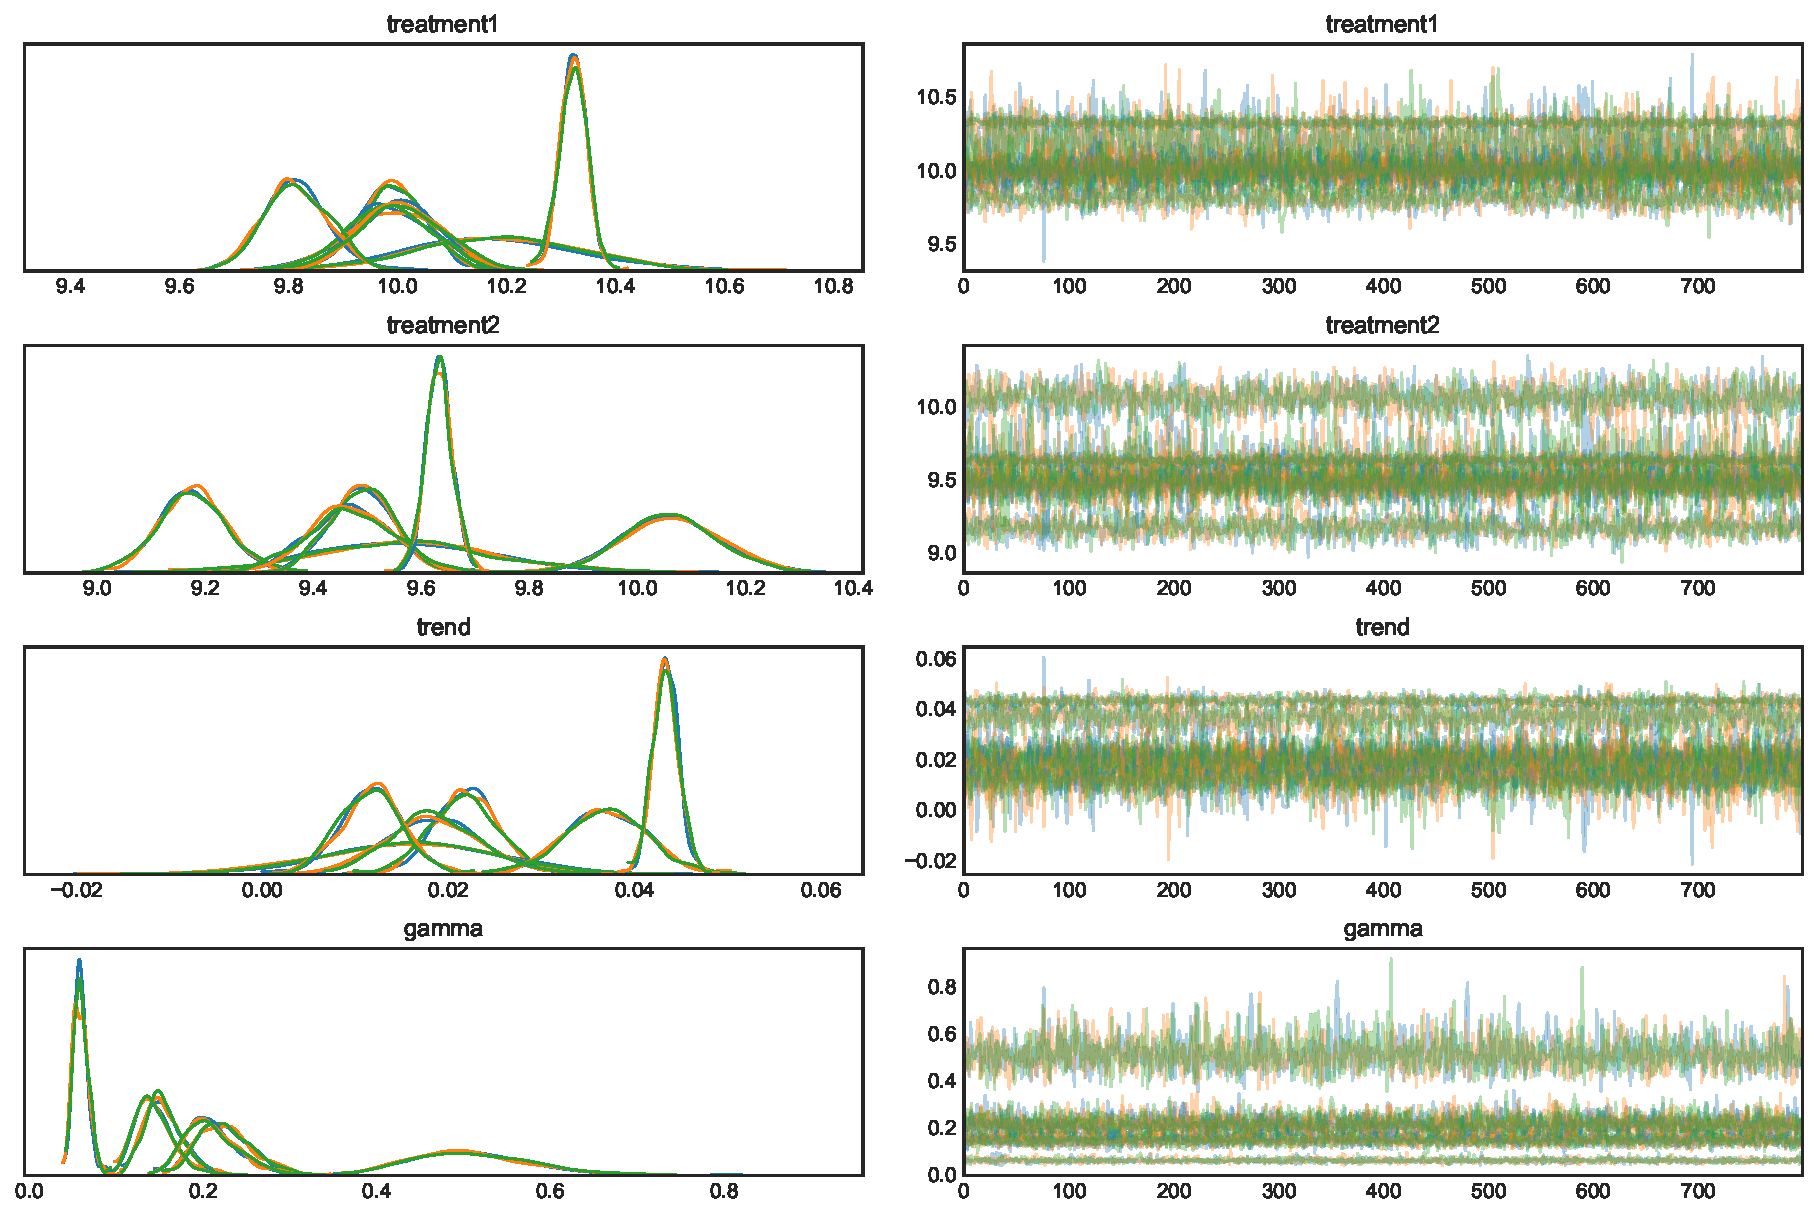
\includegraphics[width=\textwidth,height=\textheight,keepaspectratio]{hierarchical_model_patient_level_traceplot.pdf}
\end{figure}
\bigskip

Because we saw some divergences in the traceplots, it is now very important to
check the diagnostic metrics in table\ \ref{hierarchicalmodeldiagnosticmeasures} to make
sure that we don't have a problem. Effective sample size \pyv{ess_*} the effective
sample size can be in some cases less than a third of steps we took (e.g. Population
Treatment B Mean), there is still plenty enough of samples because of how long our chains were. With
\(\hat{R}\)-statistic (\pyv{r_hat}) also we don't see any problems as
the value for all parameters is 1.0, and so we can be confident that the chains have converged to
an equilibrium distribution.

\bigskip
\begin{table}[H]
    \caption{Hierarchical Model Diagnostic Metrics}\label{hierarchicalmodeldiagnosticmeasures}
    \bigskip
    \centering
    \resizebox{!}{3.2in}{%
    \begin{tabular}{lrrrrrrr}
\toprule
{} &  mcse\_mean &  mcse\_sd &  ess\_mean &  ess\_sd &  ess\_bulk &  ess\_tail &  r\_hat \\
\midrule
Population Treatment A Mean           &      0.003 &    0.002 &    1426.0 &  1426.0 &    1806.0 &    1167.0 &   1.00 \\
Population Treatment B Mean           &      0.005 &    0.004 &    1522.0 &  1522.0 &    1857.0 &    1384.0 &   1.00 \\
Population Trend Mean                 &      0.000 &    0.000 &    2045.0 &  2045.0 &    2168.0 &    1643.0 &   1.00 \\
Treatment A[0]                        &      0.001 &    0.001 &    1773.0 &  1769.0 &    1861.0 &    1591.0 &   1.00 \\
Treatment A[1]                        &      0.003 &    0.002 &    2567.0 &  2558.0 &    2640.0 &    1446.0 &   1.00 \\
Treatment A[2]                        &      0.002 &    0.001 &    1990.0 &  1990.0 &    1995.0 &    1618.0 &   1.00 \\
Treatment A[3]                        &      0.001 &    0.001 &    1850.0 &  1847.0 &    1891.0 &    1388.0 &   1.00 \\
Treatment A[4]                        &      0.002 &    0.001 &    2256.0 &  2255.0 &    2257.0 &    1418.0 &   1.00 \\
Treatment A[5]                        &      0.001 &    0.000 &    2148.0 &  2148.0 &    2160.0 &    1915.0 &   1.00 \\
Treatment B[0]                        &      0.001 &    0.001 &    2096.0 &  2092.0 &    2103.0 &    1426.0 &   1.00 \\
Treatment B[1]                        &      0.003 &    0.002 &    2594.0 &  2589.0 &    2608.0 &    1688.0 &   1.00 \\
Treatment B[2]                        &      0.002 &    0.002 &    1844.0 &  1844.0 &    1933.0 &    1624.0 &   1.00 \\
Treatment B[3]                        &      0.001 &    0.001 &    1739.0 &  1736.0 &    1793.0 &    1512.0 &   1.00 \\
Treatment B[4]                        &      0.002 &    0.001 &    2286.0 &  2284.0 &    2293.0 &    1826.0 &   1.00 \\
Treatment B[5]                        &      0.001 &    0.000 &    2300.0 &  2300.0 &    2308.0 &    1671.0 &   1.00 \\
Trend[0]                              &      0.000 &    0.000 &    1837.0 &  1837.0 &    1888.0 &    1375.0 &   1.00 \\
Trend[1]                              &      0.000 &    0.000 &    2134.0 &  2134.0 &    2206.0 &    1581.0 &   1.00 \\
Trend[2]                              &      0.000 &    0.000 &    2175.0 &  2044.0 &    2183.0 &    1233.0 &   1.00 \\
Trend[3]                              &      0.000 &    0.000 &    1734.0 &  1734.0 &    1761.0 &    1453.0 &   1.00 \\
Trend[4]                              &      0.000 &    0.000 &    1709.0 &  1709.0 &    1715.0 &    1476.0 &   1.00 \\
Trend[5]                              &      0.000 &    0.000 &    2162.0 &  2152.0 &    2184.0 &    1539.0 &   1.00 \\
Population Treatment A Sd             &      0.004 &    0.003 &    1126.0 &  1025.0 &    1602.0 &    1120.0 &   1.00 \\
Population Treatment B Sd             &      0.006 &    0.004 &    1397.0 &  1397.0 &    1996.0 &    1430.0 &   1.00 \\
Population Trend SD                   &      0.000 &    0.000 &    1436.0 &  1290.0 &    1826.0 &    1661.0 &   1.00 \\
Population Gamma                      &      0.003 &    0.003 &    2488.0 &  1342.0 &    4643.0 &    1755.0 &   1.00 \\
Gamma[0]                              &      0.000 &    0.000 &    2411.0 &  2282.0 &    2538.0 &    1666.0 &   1.00 \\
Gamma[1]                              &      0.001 &    0.001 &    2772.0 &  2594.0 &    2960.0 &    1866.0 &   1.00 \\
Gamma[2]                              &      0.001 &    0.000 &    2717.0 &  2532.0 &    2967.0 &    1808.0 &   1.00 \\
Gamma[3]                              &      0.000 &    0.000 &    2746.0 &  2503.0 &    3140.0 &    1914.0 &   1.00 \\
Gamma[4]                              &      0.001 &    0.000 &    2547.0 &  2379.0 &    2713.0 &    1663.0 &   1.00 \\
Gamma[5]                              &      0.000 &    0.000 &    2793.0 &  2498.0 &    3108.0 &    1689.0 &   1.00 \\
Population Treatment Difference (A-B) &      0.006 &    0.005 &    1616.0 &  1255.0 &    1838.0 &    1450.0 &   1.00 \\
Treatment Difference (A-B)[0]         &      0.001 &    0.001 &    3200.0 &  3180.0 &    3217.0 &    1518.0 &   1.00 \\
Treatment Difference (A-B)[1]         &      0.003 &    0.002 &    3290.0 &  3174.0 &    3263.0 &    2020.0 &   1.00 \\
Treatment Difference (A-B)[2]         &      0.002 &    0.001 &    2654.0 &  1707.0 &    2684.0 &    1438.0 &   1.00 \\
Treatment Difference (A-B)[3]         &      0.001 &    0.001 &    2882.0 &  2795.0 &    2901.0 &    1728.0 &   1.00 \\
Treatment Difference (A-B)[4]         &      0.001 &    0.001 &    3658.0 &  3597.0 &    3636.0 &    1689.0 &   1.00 \\
Treatment Difference (A-B)[5]         &      0.000 &    0.000 &    3124.0 &  3108.0 &    3121.0 &    1395.0 &   1.01 \\
\bottomrule
\end{tabular}

    }
\end{table}
\smallskip

\subsubsection*{Part 6: Checking the Posterior}

\bigskip
\begin{pyverbatim}[][fontsize=\footnotesize]
    pm.plot_posterior(
        trace,
        var_names=[
            "Population Treatment A Mean",
            "Population Treatment B Mean",
            "Population Treatment Difference (A-B)",
            "Population Trend Mean",
        ],
        credible_interval=0.95,
    )
    plt.show()
    pm.plot_posterior(
        trace,
        var_names=["Treatment Difference (A-B)"],
        credible_interval=0.95,
    )
    plt.show()
\end{pyverbatim}
\smallskip

After checking the diagnostics, now it's time to see our results. As there are
now so many parameters, we will only focus on the interesting ones. It's of course always
advisable to check every parameter to make sure that the results seem realistic,
but we skip this here for brevity and clarity.

We start with the population-level posterior that can be seen in figure\
\ref{hierarchicalmodelpopulationposteriors}. For treatment A and B treatment effect the means of the
distribution means are very close to the value that we used for simulating the data (10.1
vs 10 and 9.61 vs 9). This gives us lots of confidence that our
model is working well. It is interesting to note that the
posterior mean of the population-level treatment effects is not exactly the difference
between the posterior means 0.4, but 0.531. This is caused by the correlations between
the treatment mean posteriors. We also see that the 95 \% HPD for the difference does not include 0
so it seems that we can be quite certain that treatment B
generally works better for this population. Note though that this does not mean that we can say that it is highly
unlikely to see patients where treatment A is better because we are just looking at the
distribution of mean and not the standard deviance. To understand how likely our model
would say it is to find a patient with better efficiency with treatment A, we would need
to calculate the probability for ``drawing'' this kind of patient from a normal
distribution for each step of our chain using the value of the mean and variance in this
step and then take the average of these probabilities. With this method, we would
account for the combined uncertainty of both the mean and
the standard deviance and their possible dependencies.

\bigskip
\begin{figure}[H]
    \caption{Hierarchical Model Population-level Posterior Distributions}\label{hierarchicalmodelpopulationposteriors}
    \bigskip
    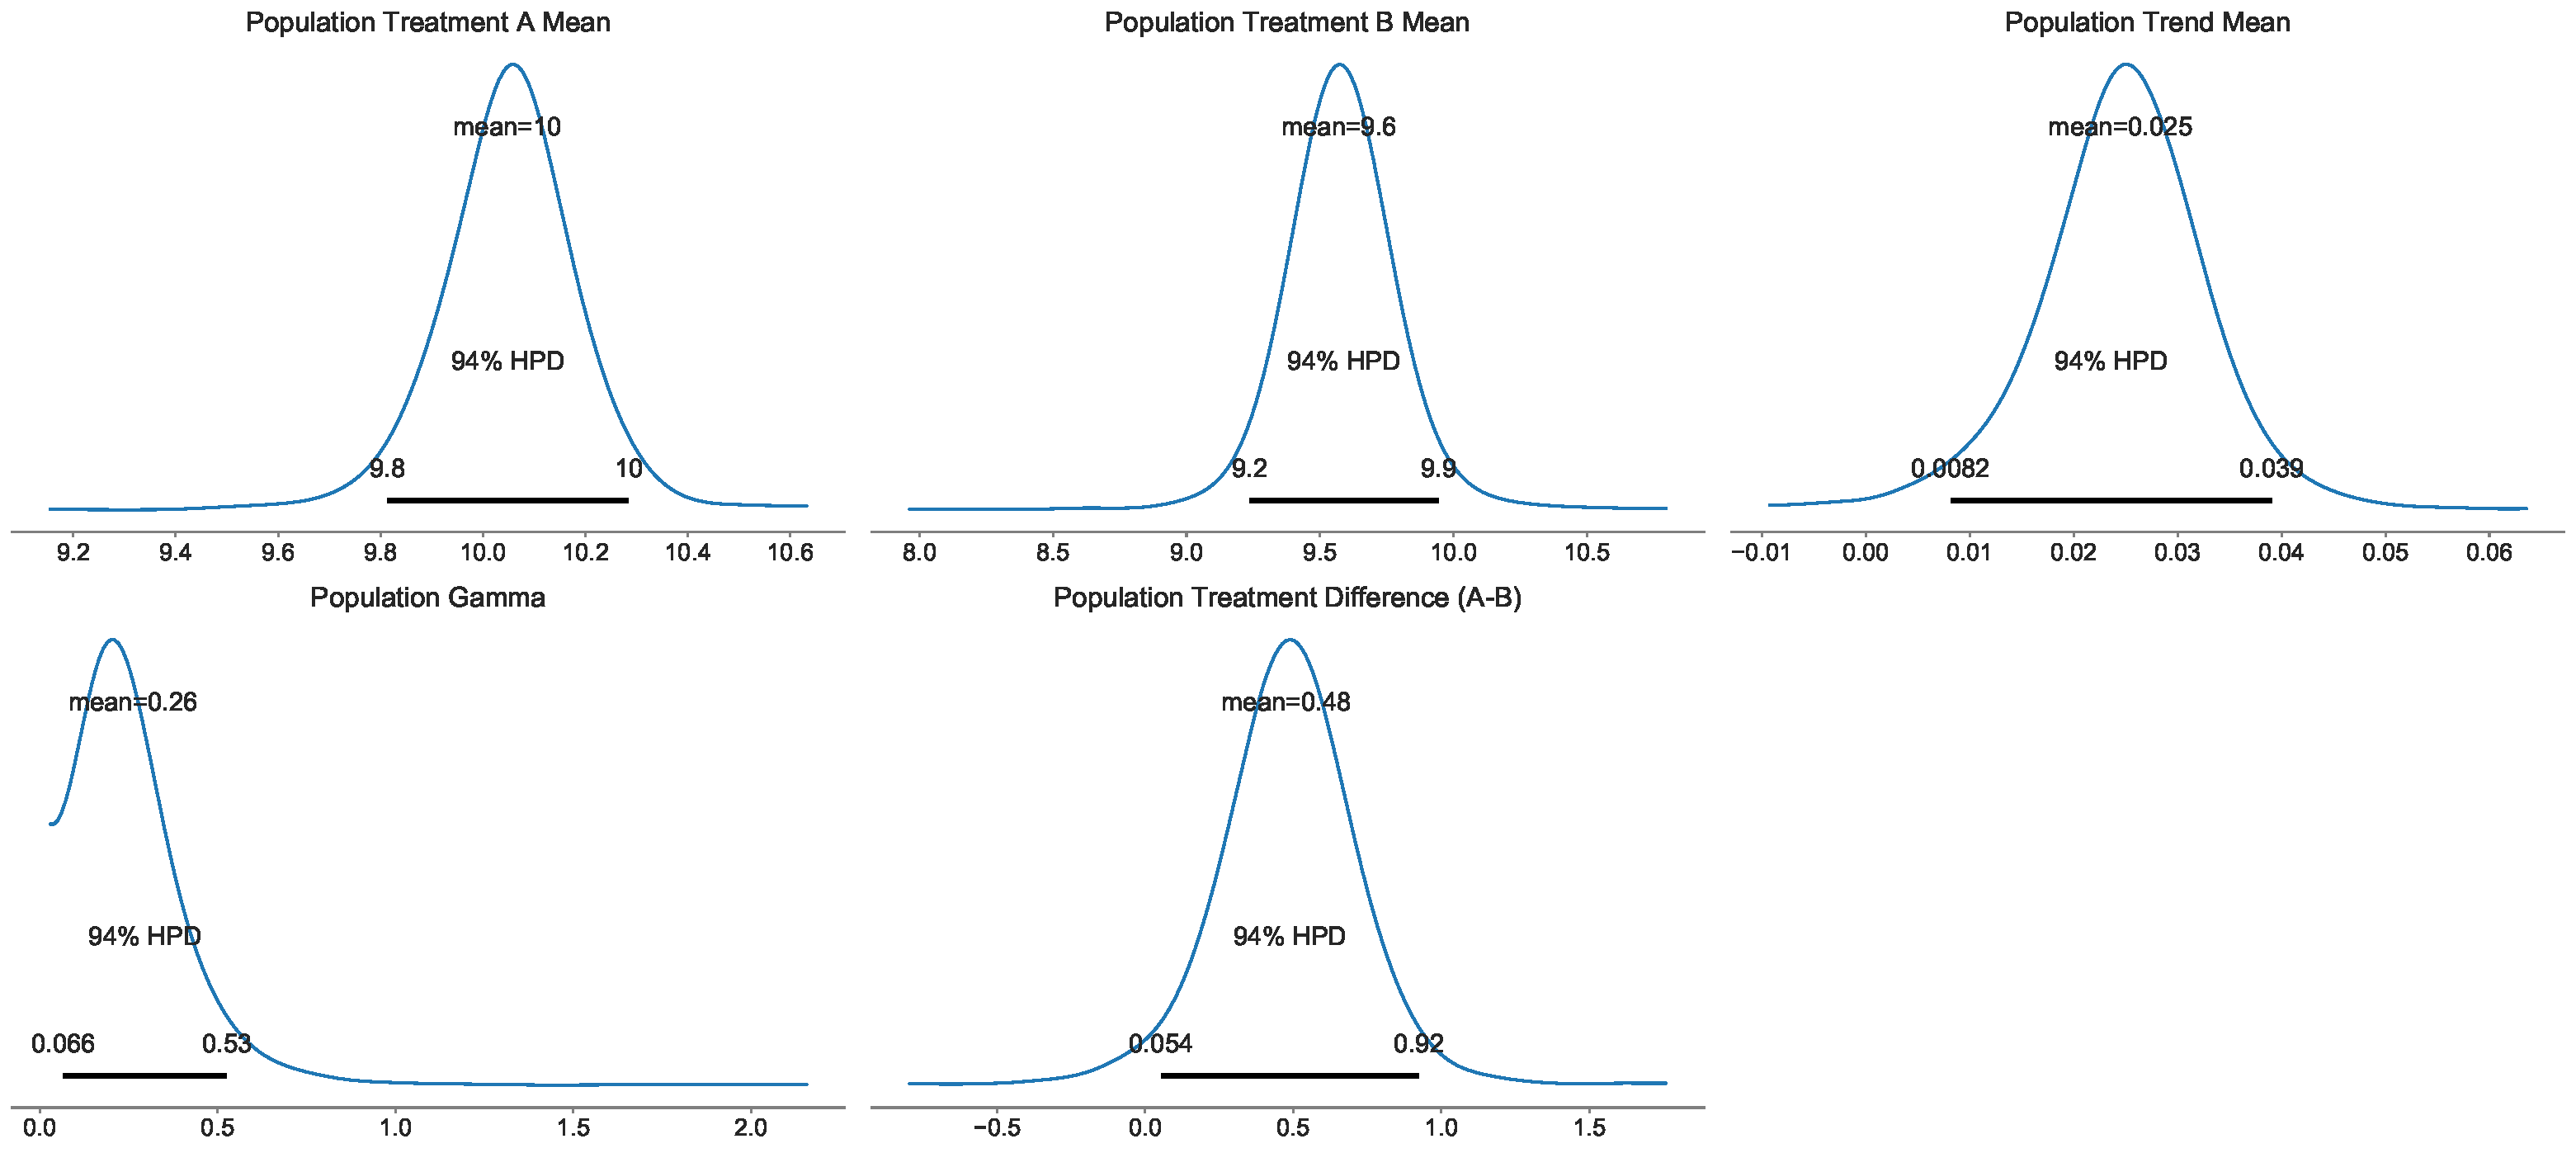
\includegraphics[width=\textwidth,height=\textheight,keepaspectratio]{hierarchical_model_population_level_posteriors.pdf}
\end{figure}
\bigskip

Now we turn to the patient-level estimates in figure\
\ref{hierarchicalmodelpatientposteriors}. Here we will focus just on the
posterior estimates of the differences of the treatments as these estimates are our
primary reason for conducting the study. We can see that for all patients
the mean value is over 0 and also 0 is not included in the 95 \% HPD, meaning that for
treatment B can be confidently recommended for all our patients.

\bigskip
\begin{figure}[H]
    \caption{Hierarchical Model Patient-level Posterior Distributions}\label{hierarchicalmodelpatientposteriors}
    \bigskip
    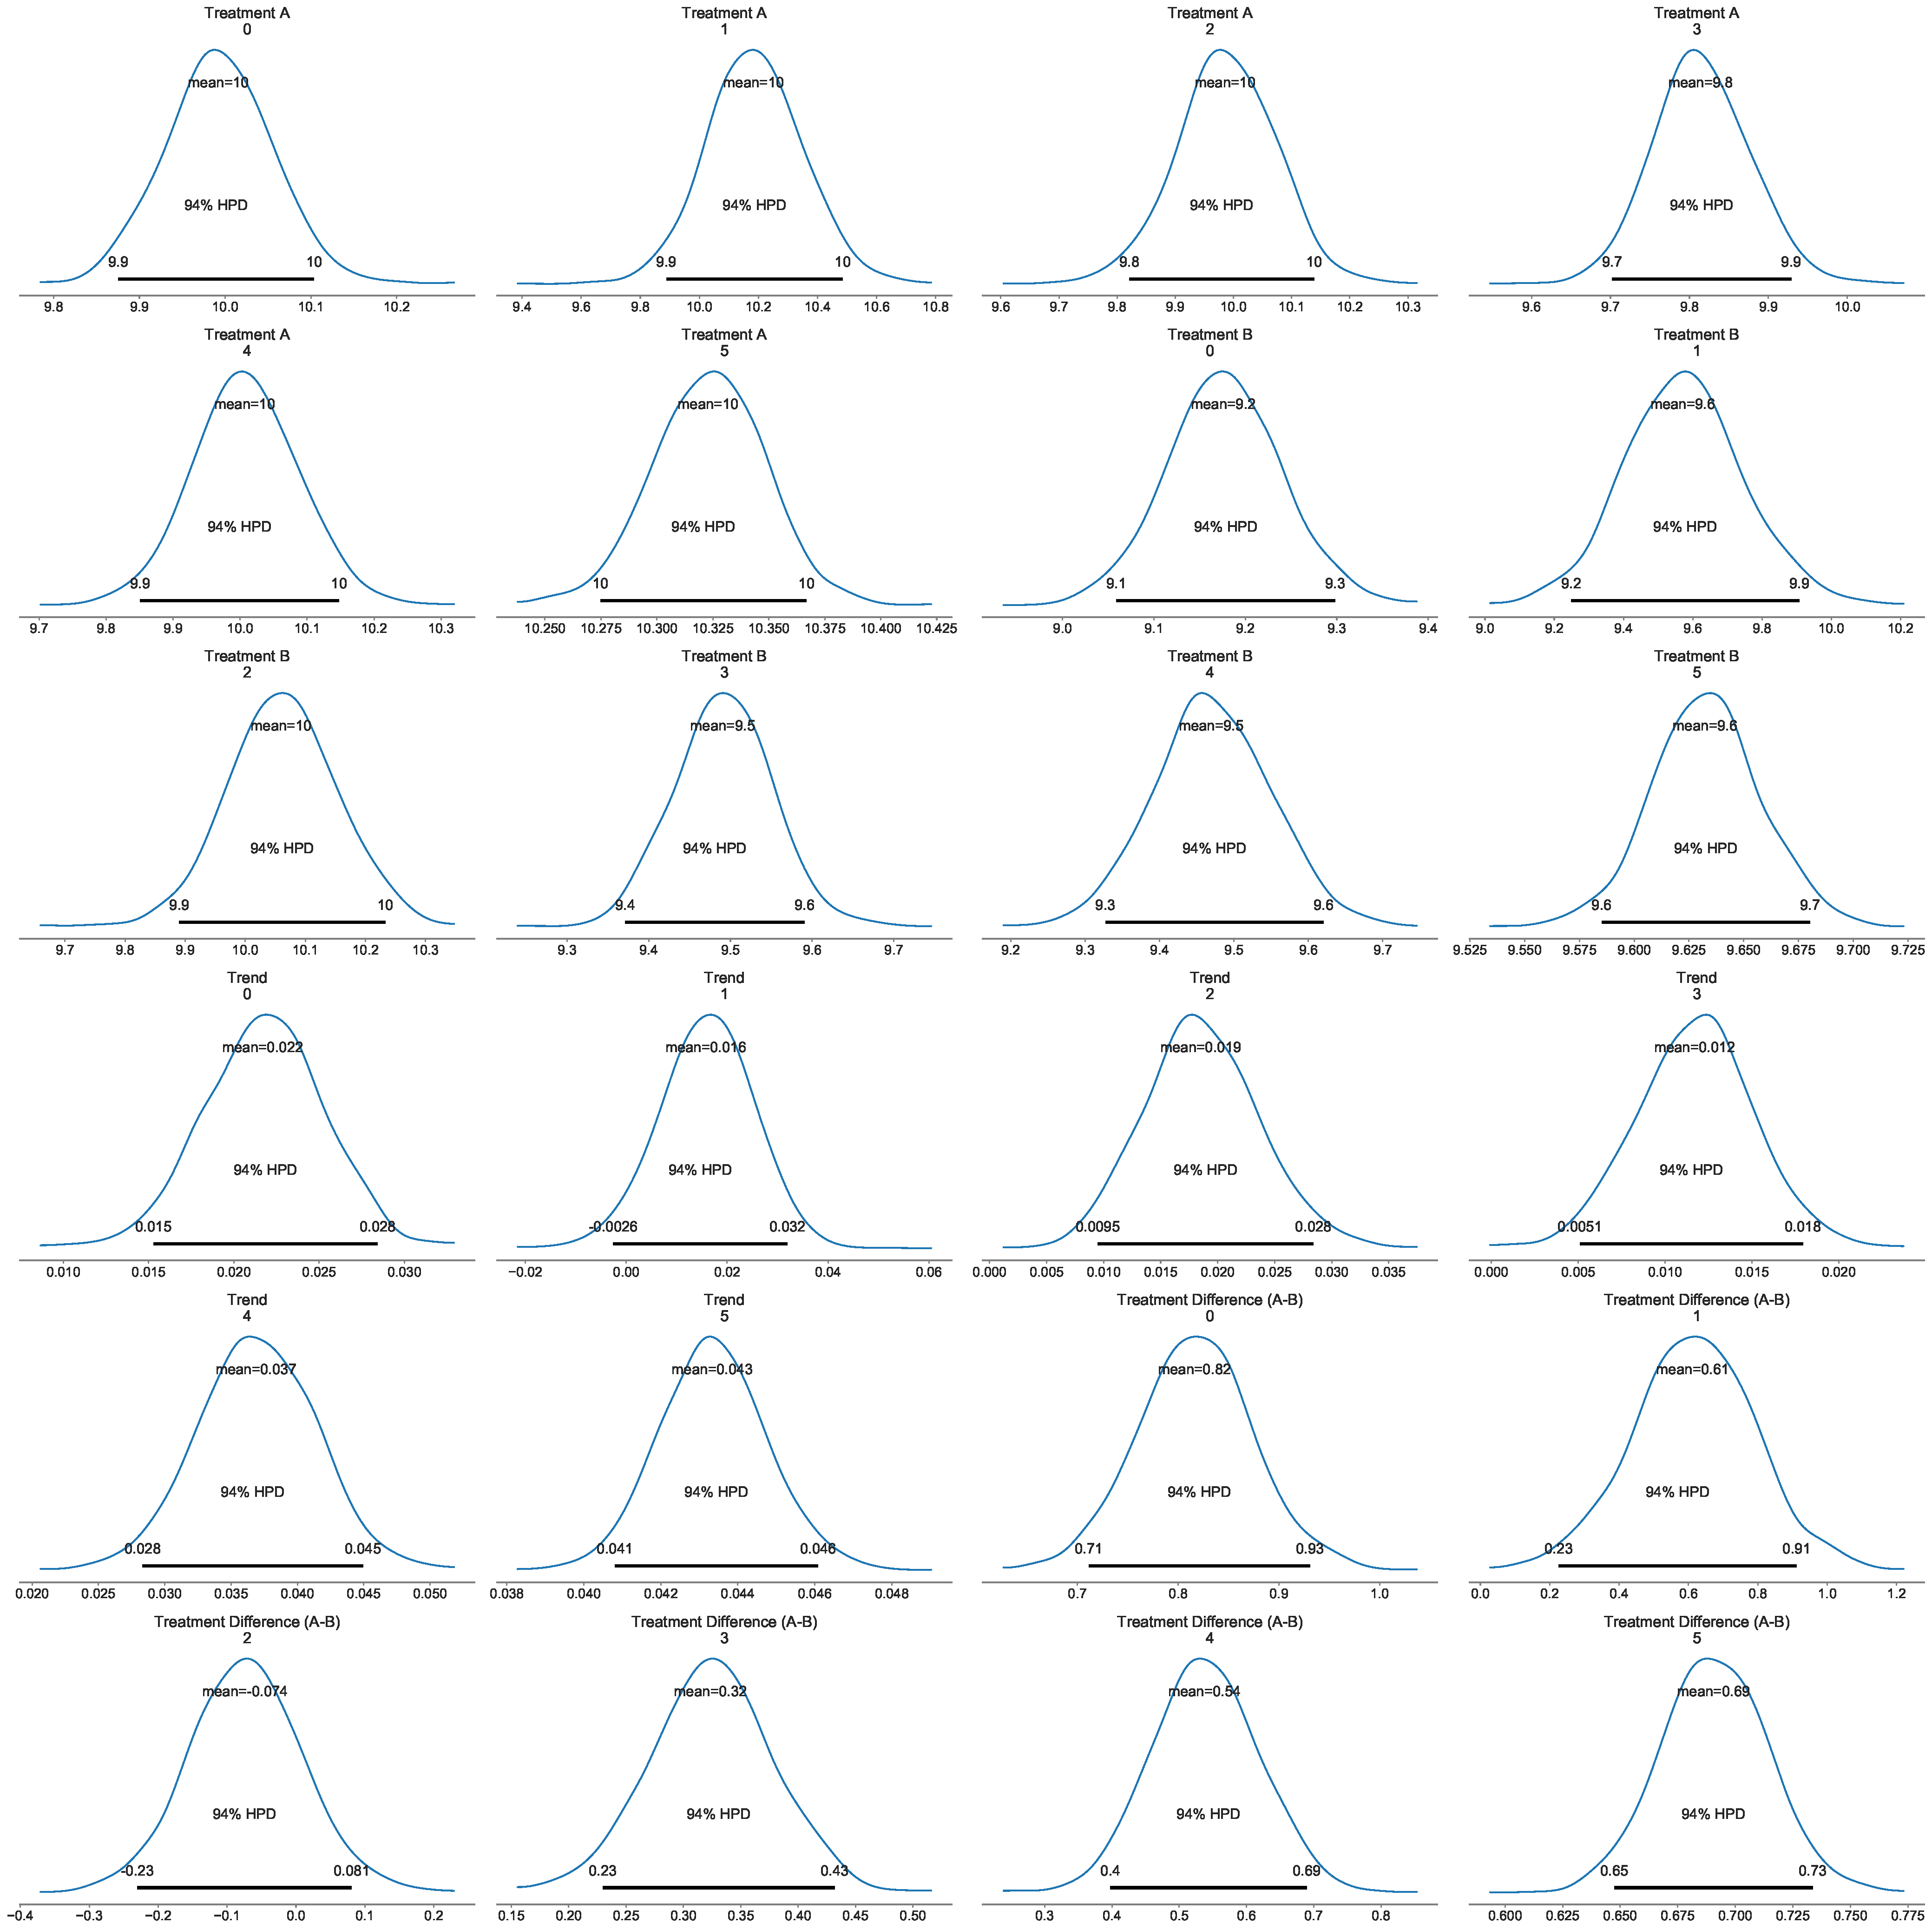
\includegraphics[width=\textwidth,height=\textheight,keepaspectratio]{hierarchical_model_patient_level_posteriors.pdf}
\end{figure}
\bigskip

\subsubsection*{Part 7: Checking Model Fit with Posterior Sampling}

\bigskip
\begin{pyverbatim}[][fontsize=\footnotesize]
with hierarchical_model as model:
    post_pred = pm.sample_posterior_predictive(trace, samples=500)
    predictions = post_pred["y"]

draw_posterior_checks(
    predictions=predictions,
    measurements_df=measurements_df,
    parameters_df=parameters_df,
)
\end{pyverbatim}
\smallskip

After seeing the results, it still necessary to do a reality check with how well the
models match the actual data. We start by once again comparing the measurements timeline
of the posterior samples to the actual measurement timeline (figure\ \ref{hierarhicalmodelposteriortimeline})

\bigskip
\begin{figure}[H]
    \caption{Hierarchical Model Posterior Sample Timeline}\label{hierarhicalmodelposteriortimeline}
    \bigskip
    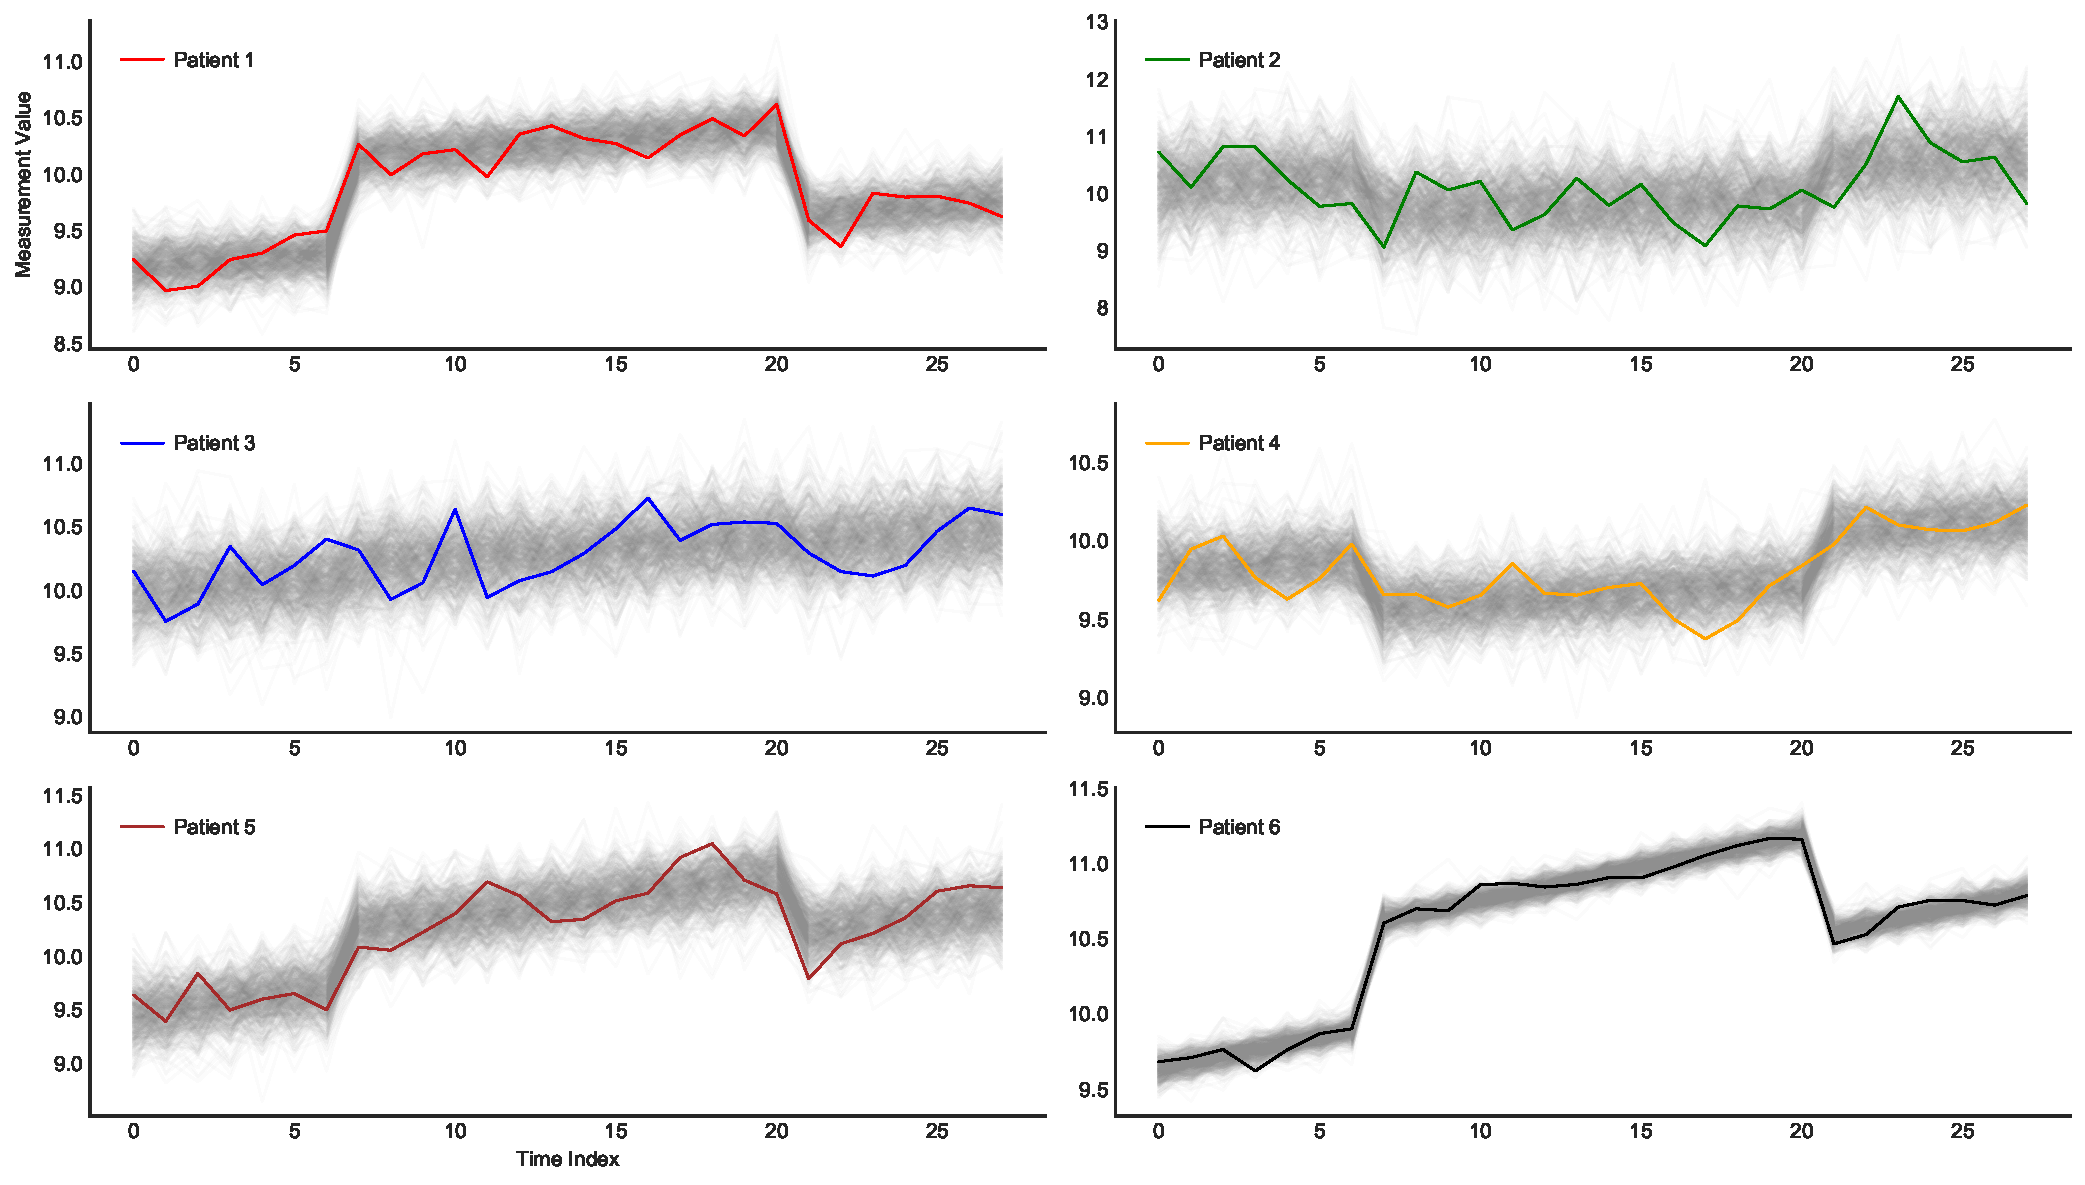
\includegraphics[width=\textwidth,height=\textheight,keepaspectratio]{posterior_sample_timeline_hierarchical_model.pdf}
\end{figure}
\bigskip

For all patients, the actual measurements lineup nicely with the samples, so our model
looks good. As we drew the plots with a shared y-axis, we also get a nice visual
representation of how the size of the measurement errors
affects the certainty of the posterior estimates. For patient 2 the measurement errors are
very big compared to other patients and the values in posterior samples
are much more spread out than for the other patients.

To get more precision into our analysis lets use our \pyv{draw_posterior_checks}
function that we also used in the single patient model. Even though the posterior
predictions that we now get from the PyMC3 inbuilt
\pyv{sample_posterior_predictive} function is structurally quite different with
multiple patients represented in the sample, our function is written
so that it can handle this new format and draw plots for each patient separately. The
resulting graphs can be seen in figure\ \ref{hierarchicalmodelposteriorsampling}.

\begin{figure}[H]
    \caption{Hierarchical Model Posterior Sample}\label{hierarchicalmodelposteriorsampling}
    \bigskip
    \centering
    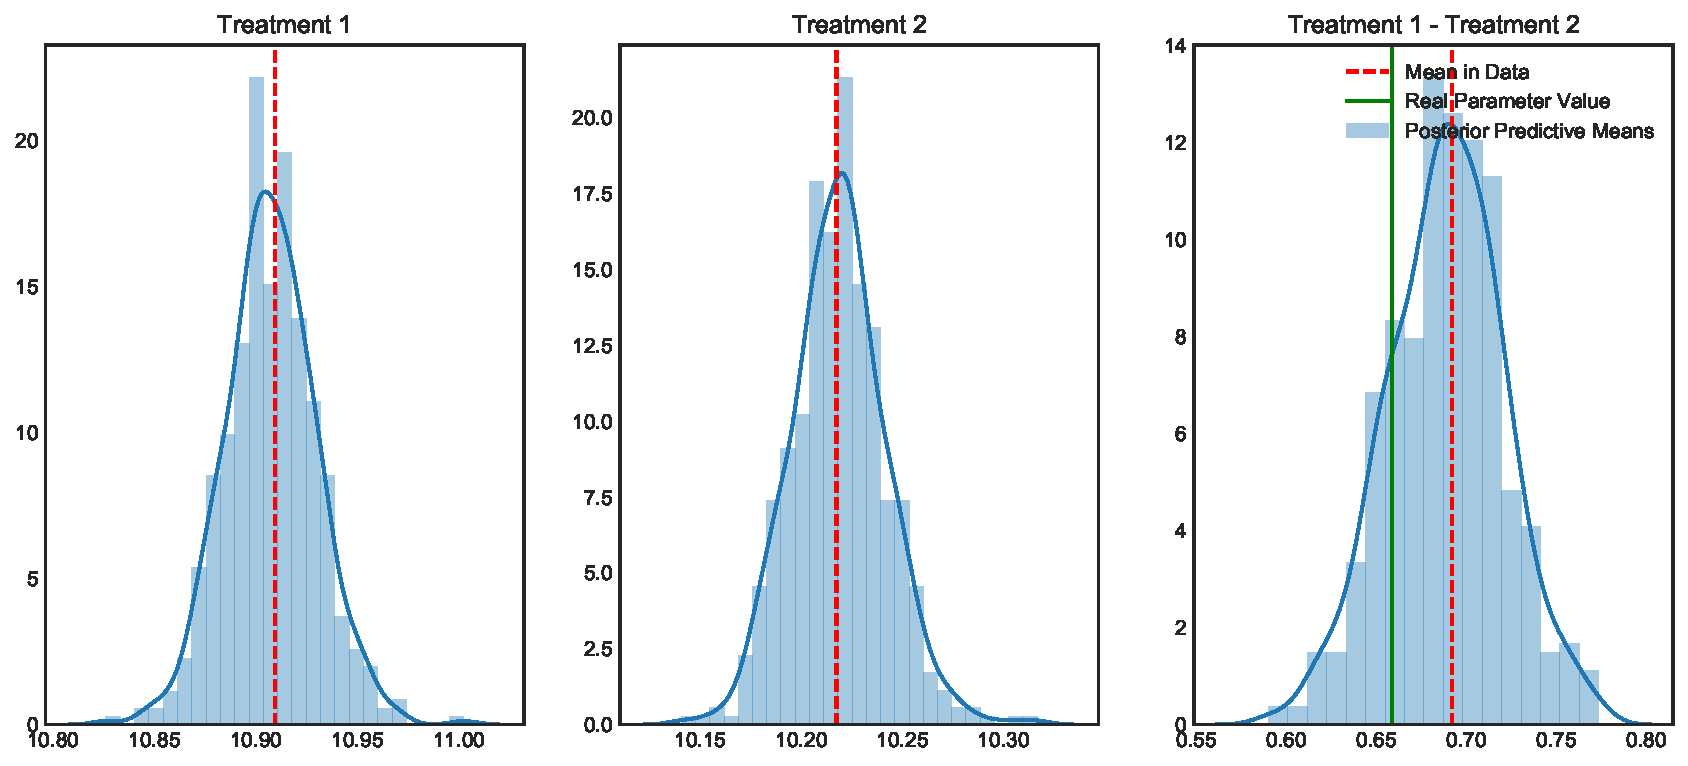
\includegraphics[width=\textwidth,height=7.6in,keepaspectratio]{hierarchical_model_posterior_sampling.pdf}
\end{figure}

What is interesting to see here is that for some patients the distribution of the
treatment means and their difference calculated from the posterior samples does not line
up nicely with the means calculated from the data. This is because of the hierarchical
nature of our model lets observations from other patients influence the estimates.
We can see that in the cases where distribution is not lined up with the
mean of the data, in most cases the distribution is shifted towards the true parameter
value. This means that our hierarchical model can somewhat correct for random
variances rising from the data creation process, by shifting the unusual patient-level
estimates towards the group modes. Even though with this model the posterior samples
don't always line up perfectly with the data with the shift towards the group mean, this
shift seems to make the estimates more accurate, so our model seems like a good enough
approximation of reality.

\subsection{Results and Interpretation}

We have now completed the hierarchical analysis. Based on the posterior estimates we can
recommend treatment B over treatment A for all the patients with high certainty
as the 95 \% HPD of the posterior of the differences in the treatment effects does not
include the value 0. The interesting question here is how did the estimates we got from
our hierarchical model differ from the single patient model and were our posterior
estimates more accurate and if so, how much and why? As this is such an important
question, let's compare the posterior estimates for treatment difference between the
single patient model and the hierarchical model for all patients by fitting the same model
we used for patient 1 for all the patients.

In figure\ \ref{modelcomparisonpatient} we can see the posterior treatment difference
distribution for all patients from the single patient model and the hierarchical model.
We can see that for all patients except patient 6 the posterior estimates got narrower
in the hierarchical model reflecting that more data was available for the estimation
through data pooling. We can also see that for patients 3 and 5 there is a clear shift in
the distribution. Although we can't see it yet from this figure, the estimates for these
patients were shifted towards the estimates of other patients. These both are indicators
of shrinkage acting in different levels, reducing the variance of estimates both in the
patient-level and between the patients.

\bigskip
\begin{figure}[H]
    \caption{Posterior Estimate of Treatment Effect Difference in Single Patient and Hierarchical Model}\label{modelcomparisonpatient}
    \bigskip
    \includegraphics[width=\textwidth,height=\textheight,keepaspectratio]{model_comparison_patient.pdf}
\end{figure}
\bigskip

To get a better view of the between patients shrinkage, where the estimates are pulled
closer to each other, let's look at mean treatment effect estimates for the two treatments.
In figure\ \ref{posteriorshrinkage} we have plotted the estimated mean of
treatment efficacy for treatment A on the x-axis and treatment B on the y-axis for
both of the models by patient. We also have also drawn in the contours of the posterior population
distribution of these values from the hierarchical model. We can clearly see that hierarchical model draws
the estimates closer together towards the population estimate centre, but it does not
draw them towards a single
mode (in this case we would see all the lines pointing a to single point). This is
because we are seeing here only the posterior estimate of two of the population-level
parameters and their mode does not necessarily represent the mode of the whole combined
population-level posterior estimate of all the parameters.

\bigskip
\begin{figure}[H]
    \caption{Hierarchical Model Posterior Sample}\label{posteriorshrinkage}
    \bigskip
    \centering
    \includegraphics[width=4.5in,height=4.5in,keepaspectratio]{posterior_shrinkage.pdf}
\end{figure}
\bigskip

The last question to consider is if the hierarchical model made our estimates more
accurate. In one way we already saw this in figure \ref{modelcomparisonpatient} where the posterior distributions were made
tighter for patient 2, reducing the uncertainty, but what we would want to know is if the
estimates of the treatment effect difference are closer to the true difference of the
parameters in the hierarchical model. For this purpose, in figure\
\ref{modelaccuracycomparison} we plot the means of posterior
estimates of the treatment effect difference for the single patient and hierarchical models
with true parameter differences by patient. We can see that the posterior means from the
hierarchical models are generally shifted closer to the true value, but this is not true
for patient 4, where the hierarchical model moves the mean to the wrong direction. The
reason for this is that the true value is not in the direction of population mode, so
the hierarchical model adjusts the estimate in the wrong direction.

\bigskip
\begin{figure}[H]
    \caption{Comparison of the Model Estimate Accuracy}\label{modelaccuracycomparison}
    \bigskip
    \centering
    \includegraphics[width=\textwidth,height=3.8in,keepaspectratio]{model_accuracy_comparison.pdf}
\end{figure}
\bigskip

Disregarding cases like patient 4, is true that making the model hierarchical will always
increase the accuracy of the model on average? Unfortunately, this is not so. Firstly our
assumption about the hierarchical nature of the data might not be correct. Constructing
a model that assumes that all patients are drawn from the same distribution, will cause
problems if that assumption is not true and estimates of some patients get adjusted towards
modes that are not representative of them. For the hierarchical model to work the
assumptions baked into its structure have to be true, or at least be an accurate enough
description of the messy reality we are trying to describe. The second thing that might make
the hierarchical model systematically less accurate is if our priors are both mistaken
and too strong. This would force conformity for the patient parameters that in reality
does not exist or prevent it from happening when it does. When thinking about the
estimation accuracy this is bad, but we could also consider this from a more Bayesian
viewpoint, with our erroneous beliefs being adjusted by the data according to the
strength of the data. In this sense, this ``problem '' is not actually a problem, but a
feature of the Bayesian method.

\chapter{Conclusion}

By bringing the focus from the group-level analysis, used in random controlled trials, to patient
level, N-of-1 experiment designs can change treatment
recommendations from one-size-fits-all to patient-specific and tailored for
each unique patient. Although this method is not currently widely
used, the combined forces of technological progress, making
health tracking easier and cheaper, and changes in the world's disease burden towards
chronic illnesses that need long term management, will likely make this method much more
popular in the future.

The design of N-of-1 trials present challenges to statistical modelling, because
of the pattern varying treatments and complex autocorrelation patterns. Although the complexity
of the data might call for a complex model, the small amount of data created from N-of-1
trials mean that it is important to keep the models only as complex as absolutely
necessary.

When estimating the parameters of the models in N-of-1 trials the setting of their use
in clinical setting mandates that focus should be on providing estimates that are
easy for a lay audience to interpret and to take into account that unplanned
changes to the designs of ongoing trials have to be accounted for. Because of these
needs, Bayesian inference can be recommended over the classical
frequentist methods as it provides an intuitive account of the uncertainty of the estimates
with highest posterior density intervals and is not tied to the trials being run always
according to a prespecified plan.

While the Bayesian methods provide advantages over the classical frequentist inference
methods, they have their own unique challenges. Instead of relying on analytical
solutions, there is often a need to use algorithmic approaches to get proper
estimates for the parameters. The need to use priors also poses its own challenges as
codifying our prior beliefs into mathematical formulas can be tricky and there is often a
conflict between the need to take into account prior information, but also let the data ``speak
for itself''.

The unique selling point for Bayesian methods in N-of-1 studies is the possibility to
make the models hierarchical and represent structures connecting different trials in the
model. This allows intelligent pooling of the data as observations from one patient can
affect the estimates for another patient, by changing our estimates about the overarching
patterns connecting the patients. This method is superior to simple data pooling
as it stays true to goals of N-of-1 trials by allowing the estimates for individual
patients to vary and only changing them when the data our prior beliefs indicate commonalities
between the patients.

Although Bayesian inference can be complicated especially when we move to hierarchical
models, the introduction of statistical packages for python and R have made the job of
the practitioner much easier, by providing ready-made solutions for the estimation
problem and easy to use model diagnostics. Even with these advances, there is still often
a need to reparametrize the model to make the job of MCMC sampler easier to get good
estimates. This is especially true in hierarchical models, but even single patient
models sometimes need adjustments.

Although this thesis tried to give a comprehensive starting point for applying Bayesian
methods for analyzing N-of-1 studies, there are certain critical aspects that we did not
have space to cover. The most important of these is data exploration. When dealing with
real-life datasets, it's unwise to jump straight into modelling before one adequately
understands the structure and patterns of the data and corrects for possible missing
values and simple errors. For a good introduction to from a graphical perspective,
interested readers are encouraged to read Nathan Yau's
``Data points: visualization that means something''\cite{dataexploration}.
The second topic we did not cover is the practice of model comparison. It is not often
the case that we can immediately come up with a model that is a good approximation of
the data creation process and often multiple models have to be tried. For a good
introduction to this topic the author recommends Chapter 10
in John Kruschke's ``Doing Bayesian Data Analysis''\cite{kruschke}.
\break
\newline
\emph{Good luck!}

\addcontentsline{toc}{chapter}{Bibliography}

\begin{thebibliography}{4}
 
    \bibitem{offset}
    Betancourt, Michael, Mark Girolami: Hamiltonian Monte Carlo for hierarchical models.
    Current trends in Bayesian methodology with applications 79.30 2015;2-4.

    \bibitem{rhatrule}
    Gabry, Jonah, Ben Goodrich: \\
    https://cran.r-project.org/web/packages/rstanarm/vignettes/rstanarm.html, 2020.
   
    \bibitem{gelman}
    Gelman, Andrew, John Carlin, Hal Stern, David Dunson, Aki Vehtari, Donald B.
    Rubin: Bayesian Data Analysis, CRC Press, 2013.

    \bibitem{variancepriors}
    Gelman, Andrew: Prior distributions for variance parameters in hierarchical models
    (comment on article by Browne and Draper). Bayesian Analysis 1.3, 2006;515-534.
    
    \bibitem{clinbayes}
    Gill, Christoper, Lora Savin, Christopher H. Schmid: Why clinicians are
    natural Bayesians, British Medical Journal 2005;330(7499):1080-1083.
    
    \bibitem{cgm}
    Hirsch, Irl, et al.: Clinical application of emerging sensor technologies
    in diabetes management: consensus guidelines for continuous glucose
    monitoring (CGM). Diabetes Technology and Therapeutics 2018;10.4:232-246.

    \bibitem{nuts}
    Hoffman, Matthew, Andrew Gelman: The No-U-Turn sampler: adaptively setting path
    lengths in Hamiltonian Monte Carlo. Journal of Machine Learning Research. 15.1,
    2014;1593-1623.

    \bibitem{github}
    Kareoja, Tuomo: https://github.com/TuomoKareoja/hierarchical-bayes-nof1-thesis,
    GitHub repository, 2020.
 
    \bibitem{HTE4}
    Kent, David, Peter Rothwell, John Ioannidis, et al.: Assessing and Reporting Heterogeneity in
    Treatment Effects in Clinical Trials: A Proposal, Trials, 2010;11:85.

    \bibitem{nofone}
    Kravitz, Richard, Naihua Duan, Sunita Vohra, Jiang Li: Introduction to
    N-of-1 Trials: Indications and Barriers in Design and Implementation of
    N-of-1 Trials: A User's Guide, AHRQ, 2014.
    
    \bibitem{kruschke}
    Kruschke, John: Doing Bayesian Data Analysis: A Tutorial With R, JAGS, and Stan
    (2nd), Academic Press, 2014.
    
    \bibitem{diseaseburden}
    Mathers, Colin, Dejan Loncar: Projections of global mortality and burden
    of disease from 2002 to 2030, PLoS medicine 2016;3.11:e442.

    \bibitem{dataexploration}
    Nathan Yau: Data points: Visualization That Means Something.
    John Wiley \& Sons, 2013.

    \bibitem{costs}
    Pace, Wilson, Elizabeth Staton, Eric Larson: Financing and Economics
    of Conducting N-of-1 Trials in Design and Implementation of N-of-1 Trials: A
    User's Guide, AHRQ, 2014.

    \bibitem{HTE1}
    Rothwell, Peter: External Validity of Randomised Controlled Trials: “To Whom Do the
    Results of This Trial Apply?”, Lancet, Jan 1-7 2005;365(9453):82-93.15.

    \bibitem{HTE2}
    Rothwell, Peter: Treating individuals 2. Subgroup Analysis in Randomised Controlled
    Trials: Importance, Indications, and Interpretation, Lancet, Jan 8-14
    2005;365(9454):176-186.16.
    
    \bibitem{pymc3}
    Salvatier, John, Thomas Wiecki, Christopher Fonnesbeck: Probabilistic Programming in Python Using PyMC3, PeerJ Computer
    Science, 2016, 2:e55.

    \bibitem{stat}
    Schmid, Christopher, Naihua Duan: Statistical Design and Analytic
    Considerations in Design and Implementation of N-of-1 Trials: A User's
    Guide, AHRQ, 2014.

    \bibitem{essbulk}
    Vehtari, Aki, Andrew Gelman, Daniel Simpson, Bob Carpenter, Paul-Christian Bürkner:
    Rank-normalization, folding, and localization: An improved $\widehat {R} $ for
    assessing convergence of MCMC. Bayesian Analysis, 2020.
   
    \bibitem{HTE3}
    Warden, Diane, John Rush, Madhukar Trivedi, et al.: The STAR*D Project Results: A Comprehensive Review of Findings, Current Psychiatry Reports, Dec 2007;9(6):449-459.
  
\end{thebibliography}
\end{document}
